\RequirePackage{xcolor}
\documentclass[shortabstract, mgr, english]{iithesis}

\usepackage{xcolor}
\usepackage[utf8]{inputenc}
\usepackage{graphicx}
\usepackage{float}
\usepackage{listings}
\usepackage{caption}
\usepackage{subcaption}
\usepackage{amsmath}
\let\lll\relax
\usepackage{amssymb}
\usepackage{enumitem}
\usepackage{booktabs}
\usepackage{hyperref}
\usepackage{url}
\usepackage{array}
\usepackage{algorithm}
\usepackage{algpseudocode}
\usepackage{tabularx}
\usepackage{multirow}
\usepackage[numbers]{natbib}

\definecolor{codebg}{RGB}{248,248,248}
\definecolor{codeframe}{RGB}{220,220,220}
\definecolor{keyword}{RGB}{0,92,197}
\definecolor{comment}{RGB}{0,128,0}
\definecolor{string}{RGB}{163,21,21}

\lstset{
  basicstyle=\ttfamily\small,
  backgroundcolor=\color{codebg},
  frame=single,
  rulecolor=\color{codeframe},
  breaklines=true,
  columns=fullflexible,
  keywordstyle=\color{keyword}\bfseries,
  commentstyle=\color{comment}\itshape,
  stringstyle=\color{string},
  showstringspaces=false,
  captionpos=b,
}

% Personal handles.
% \newcommand{\DEBUG}[1]{}     % Hide all.
\newcommand{\DEBUG}[1]{{#1}} % Display all.
\usepackage[T1]{fontenc}% Polskie literki
\newcommand{\TODO}[1]{\DEBUG{\tt{\textcolor{red}{TODO}(}{#1}{)}}}
\newcommand{\KOT}[1]{\DEBUG{\tt{\textcolor{orange}{KOT}(}{#1}{)}}}
\newcommand{\kr}{\text{\textcolor{orange}{$\blacktriangleright$}}}
\newcommand{\kl}{\text{\textcolor{orange}{$\blacktriangleleft$}}}
\newcommand{\KOTOK}[0]{\DEBUG{\tt{\textcolor{green}{OK}}}}
% Mark text changes for reviewer (red text)
\newcommand{\changed}[1]{\textcolor{red}{#1}}

\graphicspath{{img/}}

% Pinned [H] floats otherwise force LaTeX to stretch inter-paragraph glue to fill pages.
\raggedbottom

\newcolumntype{C}[1]{>{\centering\arraybackslash}m{#1}}

\polishtitle    {PCG Arena: ewaluacja i ulepszanie\fmlinebreak generatorów poziomów do gry Super Mario Bros\fmlinebreak na podstawie preferencji graczy}
\englishtitle   {PCG Arena: Evaluating and Improving\fmlinebreak Super Mario Bros Level Generators\fmlinebreak Through Player Preferences}


\polishabstract {
Ewaluacja generatorów treści proceduralnych (PCG) dla gier wideo stanowi istotne wyzwanie metodologiczne, ponieważ przyjemność gracza jest z natury subiektywna i trudna do zmierzenia za pomocą automatycznych metryk. Niniejsza praca przedstawia PCG Arenę, platformę internetową do ślepego testowania A/B generatorów poziomów do gry Super Mario Bros poprzez dane o preferencjach graczy. Super Mario Bros jest regularnie wykorzystywane jako benchmark w badaniach nad proceduralnym generowaniem poziomów od pierwszych zawodów Mario AI Competition w 2009 roku, dlatego stanowi naturalną dziedzinę do systematycznego porównywania generatorów. Platforma umożliwia graczom rozgrywanie dwóch proceduralnie generowanych poziomów obok siebie w przeglądarce, głosowanie na preferowany poziom oraz opcjonalne tagowanie cech rozgrywki. Głosy są agregowane za pomocą systemu ratingowego Glicko-2, który wyznacza rankingi wraz z przedziałami ufności.

Na podstawie zebranych danych przeprowadzono analizę eksploracyjną obejmującą ranking preferencji generatorów, statyczny zakres ekspresyjny poziomów, trajektorie rozgrywki, spójność ocen anonimowych graczy oraz semantykę tagów. Wyniki pokazują, że platforma pozwala tworzyć ranking generatorów oraz diagnozować ich typowe tryby porażki. Analiza wykazuje ponadto, że automatyczne metryki strukturalne nie są w stanie zastąpić rankingu opartego na ludzkich preferencjach, co stanowi motywację do trenowania generatora bezpośrednio na głosach graczy.

W ostatniej części pracy przedstawiono MarioDPO, generator poziomów dostrojony metodą Direct Preference Optimization, który osiąga najwyższy współczynnik zwycięstw spośród badanych generatorów i zbliża się wynikiem do oryginalnych poziomów Nintendo.
}

\englishabstract {
Evaluating procedural content generators (PCGs) for video games poses significant methodological challenges, as player enjoyment is subjective and difficult to quantify through automated metrics alone. This thesis presents PCG Arena, a web-based platform for blind A/B testing of Super Mario Bros level generators using human preference data.
Super Mario Bros has been regularly used as a benchmark for PCG level generation research since the first Mario AI Competition in 2009 and is a natural domain for systematic generator comparison. On the platform, players play two procedurally generated levels side-by-side in their browser, vote for their preferred level, and optionally tag gameplay characteristics. Votes are aggregated with the Glicko-2 rating system to produce uncertainty-aware rankings and confidence intervals.

Using the collected data, we conduct an exploratory analysis of generator preference rankings, static expressive range, gameplay trajectories, player consistency, and tag semantics. The results show that PCG Arena produces a reliable leaderboard while also diagnosing why specific generators win or fail. They further show that automated structural metrics cannot substitute for the human ranking, which motivates training a generator directly on player preferences.

Finally, we present MarioDPO, a level generator fine-tuned with Direct Preference Optimization that achieves the highest win rate among the tested procedural generators and approaches the hand-crafted Nintendo baseline.
}

\author         {Antoni Czapski}
\advisor        {dr Jakub Kowalski}
\date          {September 2026}
\transcriptnum {317214}
\advisorgen    {dr. Jakub Kowalski}

\begin{document}

\chapter{Introduction}
\label{ch:introduction}


\section{Procedural Content Generation in Video Games}
\label{sec:intro-pcg}

Procedural Content Generation (PCG) is the algorithmic creation of game
content (such as levels, maps, characters, items, and narratives) with limited or indirect
human input~\citep{togelius2011search, shaker2016pcgbook, summerville2018pcgml}. PCG has a long
commercial history: \emph{Rogue}~(1980) and \emph{Elite}~(1984) used algorithmic
generation to overcome memory constraints, and modern titles such as
\emph{Minecraft}, \emph{No Man's Sky}, and \emph{Spelunky} use procedural
generation to create replayable, large-scale worlds. Academic research on PCG has grown steadily
since the mid-2000s and spans constructive rules, evolutionary search, formal grammars, neural networks, and
reinforcement learning.

Among the game domains studied, Super Mario Bros (SMB) has accumulated the largest body of comparative work in level generation. Its 2D tile-grid format defines a
tractable design space, its physics are well understood, and the
open-source Mario AI Framework~\citep{karakovskiy2012marioai} provides a
standardised environment for both automated and human evaluation. Over 15 years
of research has produced dozens of Mario level generators across most major
PCG paradigms, yet evaluating and comparing them remains an open challenge.

Figure~\ref{fig:smb-screenshot} shows the original game and its
tile-based level geometry.

\begin{figure}[H]
\centering
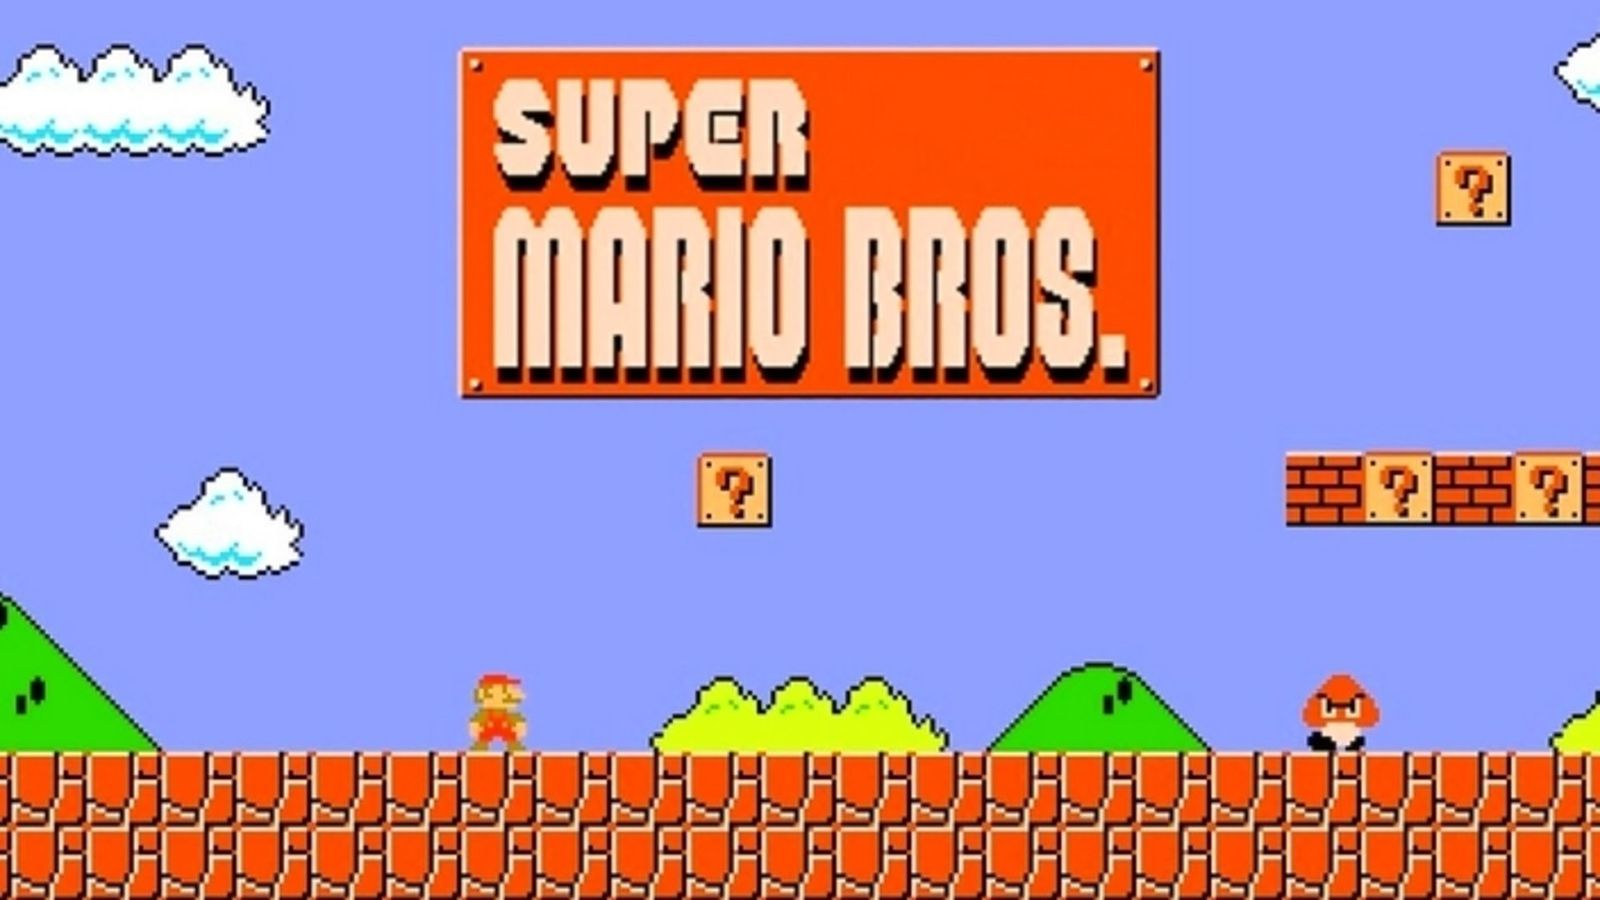
\includegraphics[width=0.75\textwidth]{smb-retro.jpg}
\caption{Screenshot of the original \emph{Super Mario Bros} (Nintendo, 1985). The player controls Mario through side-scrolling levels with platforms, enemies, power-ups, and coins. The 2D tile-grid structure of these levels defines the design space studied in this thesis.}
\label{fig:smb-screenshot}
\end{figure}

\section{The Evaluation Problem}
\label{sec:intro-evaluation-problem}

Evaluating procedural content generators is difficult because the
ultimate quality criterion, player enjoyment, is subjective and expensive to measure. The PCG literature has developed three main families of
evaluation methods, each with clear limitations.

\textbf{Automated structural metrics}, such as linearity, leniency, and density,
can be computed directly from level tilemaps and are widely used to
characterise generator output~\citep{smith2010analyzing, horn2014comparative}.
However, \citet{marino2015empirical} demonstrated that these metrics only weakly
correlate with human-rated difficulty and enjoyment, concluding that ``current
computational metrics should not be used in lieu of user studies.'' Multiple
incompatible definitions of the same metric (at least three formulations of
leniency exist in the literature) also complicate cross-study comparisons.

\textbf{Agent-based testing} uses AI controllers, typically the A* agent from
the 2009 Mario AI Championship, as player proxies. Agent-derived features such
as jump count or completion fraction provide scalable difficulty
estimates~\citep{volz2018evolving}, but superhuman agents can solve levels that
human players cannot. Difficulty estimates also depend on the specific agent policy,
which introduces a systematic bias that is rarely quantified.

\textbf{Human evaluation studies} remain the gold standard, but they are expensive and
usually small-scale: controlled lab studies use 15--37
participants~\citep{shaker2011mario, marino2015empirical}, while larger web-based
studies sacrifice experimental control~\citep{pedersen2010modeling}.
Small samples cannot control for differences in gaming experience,
player expectations, or learning effects across trials.
Existing studies were also conducted as one-time events, often years
apart, and the largest
web-based studies predate modern ML-based generators (GANs, LLMs, and diffusion
models). Many studies also reveal to participants which algorithm produced each level, even though knowing the source generator can bias player judgments.

This persistent gap between scalable-but-inaccurate automated metrics and
valid-but-expensive human studies motivates the work presented in this thesis.

\section{Research Questions and Contributions}
\label{sec:intro-rq}

This thesis addresses the PCG evaluation gap through the design, deployment, and
analysis of \emph{PCG Arena}, a web-based platform for blind A/B testing of
Mario level generators. We investigate three research questions:

\begin{description}[style=nextline]
  \item[RQ1 (Measurement)] Can a persistent, blind, web-based arena produce a
    reliable human-preference ranking of Super Mario Bros level generators?
    (Sections~\ref{sec:eda-rankings}--\ref{sec:eda-user-heterogeneity})
  \item[RQ2 (Metrics)] Can structural properties of levels explain human ranking?
    (Sections~\ref{sec:eda-static-expressive-range}--\ref{sec:dpo-judge})
  \item[RQ3 (Generation)] Can the collected preference data be used to train a
    level generator that surpasses existing PCG methods and approaches
    human-authored quality? (Chapter~\ref{ch:mariodpo})
\end{description}

\noindent The thesis makes four contributions:

\begin{enumerate}
    \item \textbf{PCG Arena}, a persistent, open-access web platform for blind
          A/B testing of Super Mario Bros level generators with
          browser-based gameplay, Glicko-2 uncertainty-aware rankings, and a
          custom matchmaking algorithm (AGIS).
    \item \textbf{A user study} of 1,000 exported pairwise votes from 77
          anonymous player IDs across 14 research generators, including 1,968
          played side records, gameplay trajectories, and descriptive
          tags.
    \item \textbf{An exploratory analysis pipeline} that connects blind preference
          votes to static expressive-range metrics, trajectory patterns,
          player-level preference profiles, and tag-based failure-mode
          diagnostics.
    \item \textbf{MarioDPO}, a level generator fine-tuned with Direct Preference
          Optimisation on arena votes that achieves a preference score of 0.832,
          close to the hand-crafted Nintendo baseline.
\end{enumerate}

The platform source code is available at
\url{https://github.com/antoniczapski/pcg-arena}.
The MarioDPO implementation, analysis scripts, and thesis sources are
available at \url{https://github.com/antoniczapski/mario-dpo}.

\section{Thesis Structure}
\label{sec:intro-structure}

The remainder of this thesis is organised as follows.
Chapter~\ref{ch:background} surveys background and related work on procedural
content generation in the context of Mario level generation, evaluation methodology,
rating systems, and preference learning. Chapter~\ref{ch:system-design} describes the design and implementation
of the PCG Arena platform. Chapter~\ref{ch:eda} presents the user
study: the study protocol and collected dataset, the generator preference
ranking and player-consistency analysis (RQ1), and an assessment of whether
static structure, gameplay behaviour, and tags can substitute for the human
ranking (RQ2). Chapter~\ref{ch:mariodpo} uses these
results (RQ3): it describes the level representation and base model, the
construction of a preference dataset from human votes and judge-labelled
synthetic pairs, DPO fine-tuning, and the evaluation of the resulting MarioDPO
generator. Chapter~\ref{ch:conclusions} summarises contributions,
discusses limitations, and outlines future directions.


\chapter{Background and Related Work}
\label{ch:background}

\section{Super Mario Bros}
\label{sec:bg-smb}

Super Mario Bros (SMB), released by Nintendo in 1985, is a side-scrolling platform
game in which the player controls Mario through a sequence of levels. Each level is
composed of a 2D tile grid, typically 16 tiles tall and 150--210 tiles wide, scrolling
horizontally from left to right. The game's design vocabulary includes several
categories of elements:

\begin{itemize}[nosep]
  \item \textbf{Terrain and platforms.} Solid ground blocks (\texttt{X}), brick blocks
        (\texttt{S}) that can be broken by hitting from below, pyramid blocks
        (\texttt{\#}), and jump-through platforms (\texttt{\%}) form the physical
        structure of each level.
  \item \textbf{Interactive blocks.} Question blocks may contain coins or power-ups:
        a Super Mushroom (which transforms Small Mario into Super Mario, allowing him
        to break bricks and survive one extra hit), a Fire Flower (enabling ranged
        attacks), or a 1-Up Mushroom (extra life). Invisible blocks provide hidden
        rewards.
  \item \textbf{Enemies.} Goombas are defeated by jumping on them; Koopa Troopas
        retract into their shells, which can then be kicked as projectiles; Spikies
        (Spinies) cannot be stomped; and Bullet Bills are fired from cannons. Winged
        variants of each enemy add vertical movement.
  \item \textbf{Collectibles.} Coins are scattered across levels as floating items or
        hidden inside blocks. Collecting 100 coins grants an extra life.
  \item \textbf{Pipes.} Decorative or functional vertical structures, some of which
        spawn Piranha Plant enemies.
  \item \textbf{Level boundaries.} Each level begins at a Mario spawn point
        (\texttt{M}) and ends at a flag pole (\texttt{F}).
\end{itemize}

The game's physics (gravity, inertia, jump arcs, and collision detection) are
deterministic and well-characterised. These properties make SMB a practical benchmark
for PCG research: the tile-grid format defines a discrete design space,
the mix of terrain, enemies, and power-ups provides a well-understood design vocabulary, and the game's familiarity means that
most experimental subjects already know the controls and goals
(Figure~\ref{fig:smb-screenshot}).

\section{Procedural Content Generation}
\label{sec:bg-pcg}

Procedural Content Generation (PCG) is the algorithmic creation of game content
with limited or indirect human input~\citep{togelius2011search, shaker2016pcgbook}. Following the
taxonomies of \citet{togelius2011search}, \citet{shaker2016pcgbook}, and \citet{summerville2018pcgml},
we distinguish five broad generation paradigms:

\begin{description}[style=nextline, leftmargin=1.5em]
    \item[Constructive / Rule-based] Sequentially place content according to
    hand-authored rules or grammars. Fast and reliable, though limited in
    expressiveness.
    \item[Search-based (SBPCG)] Frame generation as optimisation over a fitness
    function, typically using evolutionary algorithms. Flexible, though
    computationally expensive.
    \item[Grammar / Pattern-based] Use formal grammars, design patterns, or
    $n$-grams to encode structural idioms. Captures human design style,
    provided a suitable pattern library is available.
    \item[Machine Learning (PCGML)] Train neural networks on existing
    human-designed content. Data-driven and expressive, though outputs do not
    guarantee diversity or playability.
    \item[Reinforcement Learning (PCGRL)] Frame level design as a Markov
    Decision Process and train an agent to construct content. Unlike PCGML, it
    requires no corpus of existing levels and relies instead on a reward function that
    encodes the desired content properties.
\end{description}

These paradigms are not mutually exclusive, and many modern systems are hybrids. For
instance, MarioGAN~\citep{volz2018evolving} combines a learned GAN with CMA-ES
search in its latent space. A related distinction separates \emph{offline}
generation (content pre-computed before the game ships) from \emph{online}
generation (content created at runtime, potentially adapting to the player).
Online generation supports personalisation under stricter runtime
budgets, as studied in experience-driven
PCG~\citep{yannakakis2011experience}. A useful property of any generator is
\emph{controllability}: the ability to accept parameters describing desired
content features and produce matching levels.

\subsection{Search-Based Approaches}
\label{subsec:bg-search}

Search-Based PCG (SBPCG) frames content generation as an optimisation
problem~\citep{togelius2011search}. A \emph{fitness function} encodes the desired
properties of the content (e.g., playability, target difficulty, aesthetic
criteria), and an evolutionary algorithm (typically a genetic algorithm or
CMA-ES) searches a space of candidate solutions to maximise it.

Fitness functions give designers explicit, modular
control: playability constraints, difficulty targets,
and diversity objectives can be combined into a single optimisation criterion. However, SBPCG has
two well-known limitations. First, each fitness evaluation may require an
expensive simulation (e.g., running an A* agent through a candidate level).
Second, designing good fitness functions is itself a difficult problem that
mirrors the broader evaluation challenge motivating this thesis.

The Mario AI Level Generation Competition~\citep{shaker2011mario} included
several search-based entries. More recent work has applied CMA-ES to the latent
space of trained generative models~\citep{volz2018evolving} to combine
search-based and ML-based generation.

\subsection{Grammar-Based and Rule-Based Approaches}
\label{subsec:bg-grammar}

Constructive generators build content sequentially according to hand-authored
rules, typically working left-to-right through a level. The Notch generator
shipped with \emph{Infinite Mario
Bros}~\citep{karakovskiy2012marioai} is the canonical example: it iterates
through section templates (straight, hill, tubes, gaps, cannons) with fixed
selection probabilities and basic playability checks. Constructive methods are
fast and guarantee structural validity, but their expressive range is narrow.

Grammar-based approaches extend this idea by encoding design rules in a formal
grammar. \citet{shaker2012evolving} used \emph{Grammatical Evolution} (GE) to
map integer genotypes to level phenotypes via context-free grammar productions,
combining the interpretability of grammars with evolutionary search.
\citet{smith2010analyzing} introduced \emph{Launchpad}, a rhythm-based
generator that maps player actions to level geometry via a design grammar. The
same paper introduced \emph{Expressive Range Analysis} (ERA), which
generates a large sample of levels, computes structural metrics, and
visualises their joint distribution; it has since become the standard method for
characterising PCG generators.

\subsection{Machine Learning-Based Generation (PCGML)}
\label{subsec:bg-pcgml}

Machine learning approaches to PCG (PCGML) train neural networks on existing
content to learn design patterns from data~\citep{summerville2018pcgml}. Several
model families have been applied to Mario level generation.

\textbf{Sequence models.} \citet{summerville2016super} trained a 3-layer LSTM to
generate levels column-by-column using a ``snaking'' tokenisation that preserves
vertical adjacency, and co-generating levels with A*-agent play traces reached
97\% playability.

\textbf{Generative adversarial networks.} MarioGAN~\citep{volz2018evolving}
trains a Deep Convolutional GAN on sliding-window segments from a single
original SMB level. CMA-ES then searches the GAN's latent space to optimise
fitness functions based on tile distributions or agent-derived playability. This
work established the \textbf{Latent Variable Evolution} (LVE) paradigm.

\textbf{Large language models.} MarioGPT~\citep{sudhakaran2023mariogpt}
fine-tunes DistilGPT-2 on column-tokenised Mario levels with text-prompt
conditioning (e.g., ``many pipes, many enemies, low elevation''), enabling the
first natural-language-controllable level generator. 88\% of generated levels
are playable without post-processing.

\textbf{Diffusion models.} MarioDiffusion~\citep{schrum2025mariodiffusion} uses a
text-conditioned UNet denoiser to generate $16 \times 16$-tile scenes from
natural-language captions, representing the latest generation of multimodal PCG.

\textbf{Reinforcement learning.} PCGRL~\citep{khalifa2020pcgrl} formulates level
design as an MDP and trains an RL agent to edit tile grids, bypassing the need
for training data entirely.


\section{Super Mario Bros as a PCG Benchmark}
\label{sec:bg-mario}

Several practical factors explain why Super Mario Bros recurs throughout the
PCG literature: its 2D tile-grid format is compact, its
physics introduce no new mechanics after the first level (isolating level design
as the variable of interest), most players are already familiar
with the game's controls and goals, and the open-source Mario AI Framework
provides a standardised evaluation environment.

\subsection{The Mario AI Framework}
\label{subsec:bg-mario-framework}

The Mario AI Framework~\citep{karakovskiy2012marioai} is an open-source Java
implementation based on \emph{Infinite Mario Bros}, a public-domain clone of
Nintendo's Super Mario Bros created by Markus Persson in 2008. It was the
basis for three tracks of the Mario AI Championship (2009--2012):

\begin{enumerate}[nosep]
    \item \textbf{Gameplay Track}: build a controller that plays levels as well
          as possible.
    \item \textbf{Learning Track}: build a controller that learns to play.
    \item \textbf{Level Generation Track}: build software that generates levels
          for human players.
\end{enumerate}

The Level Generation Track~\citep{shaker2011mario} was the first academic PCG
competition. Generators received gameplay metrics from a test level and had
60~seconds to produce a personalised level. Six entries competed; evaluation used
pairwise forced-choice (``which was more fun?'') with 15 human judges. This
competition established several norms that influenced subsequent research:
pairwise comparison as the preferred human evaluation protocol, player telemetry
as input to adaptive generators, and the A* agent as a \emph{de facto}
playability oracle.

Levels are stored as 2D character grids (ASCII tilemaps), where each character
encodes a functional tile type. The Video Game Level Corpus
(VGLC)~\citep{summerville2016super} standardised this encoding across all 32
original SMB levels and has been widely used as training data for neural
generators.

\subsection{Mario Level Generators in the Literature}
\label{subsec:bg-mario-generators}

The PCG Arena platform hosts 14 generators spanning all major paradigm
families, selected to benchmark a broad cross-section of established PCG
approaches: one human-authored baseline, four constructive generators, one
chunk-based generator, four search-based generators, three neural generators,
and MarioDPO, the preference-aligned generator introduced in this thesis.
Table~\ref{tab:generators} provides a comparative overview.

An important caveat is that these generators do not all target the
same design vocabulary. Several reduce the problem space substantially, for
instance by restricting themselves to one or two enemy types (typically Goombas
and Green Koopas) or omitting power-ups, pipes with Piranha Plants, or
Bullet Bill cannons. This difference affects direct comparison: a generator
that uses only a subset of SMB's design elements may score well on
some structural metrics while remaining less expressive than the original
Nintendo levels.

\textbf{Human-authored baseline.} The 15 original SMB levels from Nintendo
(1985), transcribed into the Mario AI Framework's format as a reference
against which algorithmic generators are compared.

\textbf{Constructive generators.} Four generators build levels left-to-right
using probabilistic placement: the \emph{Notch} generator shipped with Infinite
Mario Bros, its \emph{Parameterized} variant (NotchParam) exposing six tunable
difficulty and style parameters~\citep{shaker2011mario}, a \emph{Randomized} variant
(NotchParamRand) that randomly samples parameters per level, and \emph{Hopper},
which alternates generated and pre-designed segments with adaptive probability
adjustment.

\textbf{Chunk-based assembly.} \emph{Occupancy-Regulated Extension}
(ORE)~\citep{mawhorter2010occupancy} builds levels by iteratively attaching
hand-authored chunks at compatible anchor points.

\textbf{Search-based generators.} The \emph{Grammatical Evolution} (GE)
generator~\citep{shaker2012evolving} evolves level-construction programs via a
context-free grammar. Three \emph{Pattern-based}
generators~\citep{dahlskog2014procedural} represent levels as sequences of
micro-patterns extracted from original SMB levels and use evolutionary search
with different fitness functions: pattern count (maximising motif frequency),
pattern occurrence (maximising motif diversity), and weighted pattern count
(rewarding rare motifs).

\textbf{Neural generators.} \emph{MarioGAN}~\citep{volz2018evolving} combines a
DCGAN with CMA-ES latent-space search.
\emph{MarioGPT}~\citep{sudhakaran2023mariogpt} uses a fine-tuned DistilGPT-2
with text-prompt control;
\emph{MarioDiffusion}~\citep{schrum2025mariodiffusion} generates tile scenes from
natural-language captions via a diffusion model; and \emph{MarioDPO}, introduced in Chapter~\ref{ch:mariodpo}, fine-tunes a GPT-2-based generator with Direct Preference
Optimisation on PCG Arena votes.

\begin{table}[H]
\centering
\footnotesize
\begin{tabular}{@{} l l l l r @{}}
\toprule
\textbf{Generator} & \textbf{Paradigm} & \textbf{Key technique} & \textbf{Control} & \textbf{Year} \\
\midrule
Original SMB1      & Human        & Manual design               & ---            & 1985 \\
Notch              & Constructive & Probabilistic L-to-R        & None           & 2008 \\
NotchParam         & Constructive & Probabilistic + 6 params    & Param.\ knobs  & 2011 \\
NotchParamRand     & Constructive & Probabilistic + random      & Random         & 2011 \\
Hopper             & Constructive & Adaptive probabilistic      & Adaptive       & 2010 \\
ORE                & Chunk-based  & Anchor-point assembly       & None           & 2010 \\
GE                 & Search       & Grammatical evolution       & Via grammar    & 2012 \\
Pattern Count      & Search       & Evolutionary (pattern freq.)& Fitness wts.   & 2014 \\
Pattern Occurrence & Search       & Evolutionary (unique patt.) & Fitness wts.   & 2014 \\
Pattern Wt.\ Count & Search       & Evolutionary (rarity-wt.)   & Fitness wts.   & 2014 \\
MarioGAN           & ML (GAN)     & DCGAN + CMA-ES latent       & Fitness fn.    & 2018 \\
MarioGPT           & ML (LLM)     & Fine-tuned DistilGPT-2      & Text prompts   & 2023 \\
MarioDiffusion     & ML (Diff.)   & Text-conditioned UNet       & Text captions  & 2025 \\
MarioDPO           & ML + DPO     & GPT-2 + pref.\ alignment    & Text + DPO     & 2026 \\
\bottomrule
\end{tabular}
\caption{Generators included in PCG Arena. All except MarioDPO (this thesis) are
previously published or reference implementations.}
\label{tab:generators}
\end{table}

By including generators from all paradigm families and spanning nearly four
decades of game content creation, PCG Arena tests whether human preference data
can discriminate generator quality more reliably than automated metrics.


\section{Evaluation Methods for Procedural Content}
\label{sec:bg-evaluation}

Evaluation is the central methodological challenge in PCG research and the
primary motivation for PCG Arena. This section surveys the main families of
evaluation methods used in the Mario PCG literature.

\subsection{Automated Metrics}
\label{subsec:bg-eval-automated}

The most widely used evaluation approach computes \emph{static structural
metrics} directly from the tile grid, without simulating gameplay.

\textbf{Linearity} measures how closely a level's vertical profile follows a
straight line. \citet{smith2010analyzing} defined it as the mean
absolute residual (the average vertical distance between platform midpoints
and the best-fit regression line), so lower values indicate a more linear
level. Later works~\citep{horn2014comparative,
summerville2017understanding} instead use $R^2$ (the coefficient of determination, measuring
the proportion of variance in the data explained by the regression), which inverts the scale so that higher $R^2$ means more linear. Because the two formulations are not directly comparable, complicating cross-paper analyses.

\textbf{Leniency} approximates difficulty through weighted sums of game objects.
In its original form~\citep{smith2010analyzing}, it is computed as
$L = (w_p \cdot n_p + w_g \cdot n_g + w_e \cdot n_e) / W$, where $n_p$ is the
number of power-ups, $n_g$ the number of gaps, $n_e$ the number of enemies, $W$
the level width in tiles, and the weights $w_p > 0$, $w_g, w_e < 0$ reward
forgiving content and penalise hazards. At least three incompatible formulations exist in the literature, using different
tile weights and normalisation schemes~\citep{smith2010analyzing,
shaker2012evolving, marino2015empirical}, and
\citet{marino2015empirical} showed that leniency only weakly correlates with
human-rated difficulty.

\textbf{Compression distance} (gzip-based Normalised Compression Distance)
quantifies structural similarity between level pairs and is used as a diversity
proxy~\citep{shaker2012evolving, horn2014comparative}.

\textbf{Expressive Range Analysis} (ERA), introduced by
\citet{smith2010analyzing}, generates a large sample of levels, computes two
metrics per level (classically linearity vs.\ leniency), and plots their joint
distribution as a 2D histogram. ERA has been widely adopted~\citep{horn2014comparative,
shaker2012evolving}, though it remains purely descriptive and characterises what a
generator produces without indicating whether players enjoy it.
An ERA characterisation of the PCG Arena generators is
presented in Section~\ref{sec:eda-static-expressive-range}
(Figure~\ref{fig:eda-expressive-range}).

\subsection{Agent-Based Testing}
\label{subsec:bg-eval-agents}

AI agents used as player proxies allow scalable, repeatable assessment of
playability and difficulty.

\textbf{Playability gates.} A level is deemed playable if a strong A* agent can
complete it. This binary check is the most common first stage in PCG evaluation
pipelines~\citep{volz2018evolving, summerville2016super, khalifa2020pcgrl}.

\textbf{Difficulty proxies.} Agent-derived metrics include jump count (the
number of jumps the A* agent performs, interpreted as difficulty), completion
fraction (progress along the $x$-axis if the level is not fully completable),
and virtual damage from stochastic ``human-like'' agents that model input timing
inaccuracies~\citep{nam2024using}.

Agent-based evaluation is fast and reproducible, but
agent bias is a central concern: superhuman agents can solve levels humans
cannot, and difficulty estimates depend on the specific agent policy. The mismatch also goes the other way:
many levels that human players can complete are unsolvable by standard A* agents,
which lack the ability to backtrack, use special power-ups, or exploit advanced
movement techniques. These bi-directional limitations are rarely quantified in
the literature.

\subsection{Human Evaluation Studies}
\label{subsec:bg-eval-human}

Human studies remain the gold standard for PCG evaluation but vary widely in
scale and methodology.

\textbf{Pairwise forced-choice.} The Mario AI
Championship~\citep{shaker2011mario} asked 15 judges to play two levels and
select ``which was more fun?'' without further defining ``fun.'' This protocol
directly inspired PCG Arena's design.

\textbf{Likert-scale ratings.} \citet{marino2015empirical} used 7-point Likert
scales (ordered response scales from ``strongly disagree'' to ``strongly agree'')
for enjoyment, aesthetics, and difficulty with $n = 37$ participants. 
\citet{summerville2017understanding} collected ratings across 85 design metrics
and showed that inter-rater agreement imposes ceilings on achievable
metric--human correlations. An automated metric cannot correlate with human ratings any better
than humans correlate with each other, so reporting an inter-rater agreement
baseline is important when interpreting metric--human correlations.


\textbf{Large-scale web studies.} \citet{pedersen2010modeling} collected
240~game pairs via a web deployment of \emph{Infinite Mario Bros} variants
for pairwise affective-preference analysis.
A follow-up by \citet{shaker2011features} collected 600
game-pair comparisons via an uncontrolled web applet, though the number of unique
participants was not reported.
Both studies date from 2010--2011 and predate ML-based generators
such as GANs, LSTMs, and diffusion models.

These studies show that while human empirical evaluation provides the
most direct quality signal, it is expensive, typically small-scale ($n < 40$ in
controlled settings), and conducted as isolated, one-time events.
Earlier work on automatic personalised content
generation~\citep{shaker2010towards} and design-pattern
analysis~\citep{dahlskog2013patterns} explored the relationship between
level structure and player preferences, but likewise relied on small participant
pools.
Because the largest prior web studies were conducted before modern
neural generators existed, contemporary Mario level generators have not yet been compared systematically in a shared human study.

\subsection{Comparison of Approaches and Their Limitations}
\label{subsec:bg-eval-comparison}

Table~\ref{tab:eval-comparison} summarises the evaluation methods employed across
the most representative papers in the Mario PCG literature.

\begin{table}[H]
\centering
\small
\begin{tabular}{lllccccc}
\toprule
\textbf{Paper} & \textbf{Year} & \textbf{PCG algorithm} & \textbf{S} & \textbf{A} & \textbf{ERA} & \textbf{H} & \textbf{ML} \\
\midrule
Smith \& Whitehead          & 2010 & Launchpad (rhythm-based) & $\checkmark$ &              & $\checkmark$ &              &              \\
Pedersen et al.             & 2010 & Notch (parameterised)   & $\checkmark$ &              &              & $\checkmark$ & $\checkmark$ \\
Shaker et al.\ (Champ.)     & 2011 & Comp.\ entries (mixed)  & $\checkmark$ & $\checkmark$ &              & $\checkmark$ &              \\
Shaker et al.\ (GE)         & 2012 & Grammatical Evolution   & $\checkmark$ &              & $\checkmark$ &              &              \\
Horn et al.                 & 2014 & Multiple (comparative)  & $\checkmark$ &              & $\checkmark$ &              &              \\
Marino et al.               & 2015 & GE + Notch (compared)   & $\checkmark$ &              &              & $\checkmark$ &              \\
Summerville \& Mateas       & 2016 & LSTM column generator   & $\checkmark$ & $\checkmark$ &              &              & $\checkmark$ \\
Summerville et al.          & 2017 & Multiple (8 generators) & $\checkmark$ & $\checkmark$ &              & $\checkmark$ & $\checkmark$ \\
Volz et al.\ (MarioGAN)     & 2018 & DCGAN + CMA-ES          & $\checkmark$ & $\checkmark$ &              &              &              \\
Nam et al.                  & 2024 & Stochastic ``human-like'' agents & $\checkmark$ & $\checkmark$ &              & $\checkmark$ &              \\
\midrule
\textbf{PCG Arena (ours)}   & \textbf{2026} & \textbf{14 generators (all paradigms)} & $\checkmark$ & $\checkmark$ & $\checkmark$ & $\checkmark$ & $\checkmark$ \\
\bottomrule
\end{tabular}
\caption{Evaluation methods used in Mario PCG research.
  S\,=\,structural metrics;
  A\,=\,agent-based;
  ERA\,=\,Expressive Range Analysis;
  H\,=\,human study;
  ML\,=\,learned predictor.}
\label{tab:eval-comparison}
\end{table}

The works in Table~\ref{tab:eval-comparison}
show how Mario PCG evaluation has developed from structural
analyses, through agent-based playability checks and expressive-range
characterisations, to small-scale human studies and learned predictors of
player behaviour. Across this body of work, three recurring problems stand out:

\textbf{Metrics--experience misalignment.} \citet{marino2015empirical} showed
that two generators rated identically by all computational metrics were rated
\emph{significantly differently} by human players on enjoyment.
\citet{summerville2017understanding} further demonstrated that inter-rater
agreement imposes ceilings on achievable metric--human correlations, with
aesthetics being particularly noisy. Automated metrics are useful
characterisation tools, but they are unreliable proxies for perceived quality.

\textbf{Small-$n$ and one-time studies.} Most human studies use 15--37
participants in controlled settings and were conducted as isolated events, often
years apart. Moreover, when evaluations are not blind and players know which algorithm produced a level, prior
expectations can bias their judgments.

\textbf{Absence of a community-standard reward model.} Search-based and
RL-based generators require fitness or reward functions, yet no validated reward
model for Mario level quality exists because human preference data across diverse generators has been unavailable.

PCG Arena addresses these gaps with a persistent, blind, web-based
platform for human evaluation. The collected preferences can be used to
(a)~rank generators with statistical confidence, (b)~test whether automated
metrics correlate with human judgment, and
(c)~train preference-aligned generators.


\section{Rating Systems for Pairwise Comparisons}
\label{sec:bg-rating}

PCG Arena uses pairwise comparisons as its primary data collection protocol.
This section reviews the mathematical foundations underlying the platform's
rating engine.

\subsection{The Elo Rating System}
\label{subsec:bg-elo}

Modern skill-rating systems build on the \emph{Bradley-Terry
model}~\citep{bradley1952rank}: each item $i$ is assigned a strength parameter
$\pi_i$, and the probability that item $i$ is preferred to item $j$ is
%
\begin{equation}
\label{eq:bt}
P(i \succ j) = \frac{\pi_i}{\pi_i + \pi_j}.
\end{equation}

\citet{elo1978rating} operationalised this model for competitive chess. Each
player carries a scalar rating $R$; the expected score of player~$A$ against
player~$B$ is
%
\begin{equation}
\label{eq:elo}
E_A = \frac{1}{1 + 10^{(R_B - R_A)/400}}.
\end{equation}

After an observed outcome $S_A \in \{0, 0.5, 1\}$, the rating updates as
$R_A' = R_A + K(S_A - E_A)$, where $K$ is a fixed gain constant. Elo's
simplicity made it the standard in chess, tennis, and early online games, but a
constant $K$ cannot distinguish a well-established rating from a newcomer's. Bayesian extensions address this limitation by tracking rating uncertainty explicitly.

\subsection{The Glicko-2 Rating System}
\label{subsec:bg-glicko2}

\citet{glickman1999parameter} recast Elo in a Bayesian framework
(\emph{Glicko}), modelling each player's rating as a Gaussian
$\mathcal{N}(\mu, \sigma^2)$ where the \emph{rating deviation} (RD)
$\sigma$ quantifies uncertainty. Between rating periods, RD grows to reflect
increased uncertainty from inactivity.

\emph{Glicko-2}~\citep{glickman2012glicko2} extends Glicko with a third
parameter, \emph{volatility}~$\sigma_v$, which captures how erratic an entity's
performance is. The update pipeline converts ratings to an internal scale,
estimates variance and improvement from outcomes, iteratively updates volatility,
and then updates RD and rating. On the internal Glicko-2 scale the rating
deviation is denoted $\phi = \text{RD} / \lambda$, where
$\lambda = 173.7178$ is the scale conversion factor:
%
\begin{align}
\phi' &= \frac{1}{\sqrt{1/\phi^{*2} + 1/v}}, \quad
  \text{where } \phi^* = \sqrt{\phi^2 + \sigma_v'^{\,2}},
  \label{eq:glicko-rd-bg} \\
\mu' &\leftarrow \mu + \phi'^2 \sum_j g(\phi_j)(s_j - E_j),
  \label{eq:glicko-mu-bg}
\end{align}
%
where $g(\phi) = 1/\sqrt{1 + 3\phi^2/\pi^2}$ down-weights predictions
involving uncertain opponents, $s_j$ is the observed outcome, and $E_j$ the
expected outcome.

PCG Arena uses Glicko-2 with generators and levels treated as ``players'': each
human vote corresponds to a match outcome. RD provides a built-in measure of
rating reliability, and volatility accommodates generators whose perceived
quality shifts as new levels are added. Implementation details and parameter
choices are described in Section~\ref{sec:sd-rating}.

\subsection{Arena-Style Evaluation Platforms}
\label{subsec:bg-arenas}

The \emph{arena paradigm}, in which anonymous pairwise votes from a crowd are used
to rank competing systems, has also been adopted outside games.
In \emph{Chatbot Arena}, \citet{chiang2024chatbot} deployed a web platform where
users chat simultaneously with two anonymous LLMs and vote for the better
response. Over 240,000 votes from more than 90,000 users have been collected, and rankings are
computed via Bradley-Terry MLE. An active sampling strategy concentrates votes on
close model pairs, using information-gain ideas similar to PCG
Arena's AGIS algorithm. Chatbot Arena is the closest structural analogue to PCG
Arena outside the games domain.

A complementary direction is \emph{LLM-as-a-Judge}: \citet{zheng2023judging} studied using GPT-4 as a
surrogate judge for pairwise evaluation and reported over 80\% agreement with human
preferences. PCG Arena's \emph{Judge Function} plays a similar role on a
smaller scale as a heuristic filter for labelling additional level pairs
(Section~\ref{sec:dpo-judge}).

In the games domain, \citet{sarkar2017glicko2} applied Glicko-2 to the human computation game
\emph{Paradox}, treating puzzle tasks as rated entities alongside players;
this is a direct precedent for PCG Arena's use of Glicko-2 to rate
game content.
More broadly, \citet{snow2008cheap} showed that aggregating labels from multiple non-expert
annotators can match expert-level quality, supporting the assumption
that a sufficient number of non-expert pairwise votes yields a reliable ranking.


\section{Preference Learning and Alignment}
\label{sec:bg-alignment}

PCG Arena's preference data supports both generator ranking and active
generator improvement via preference learning. This section reviews two main
approaches: Reinforcement Learning from Human Feedback (RLHF) and its
simplified successor, Direct Preference Optimisation (DPO).

\subsection{Reinforcement Learning from Human Feedback}
\label{subsec:bg-rlhf}


RLHF trains a policy to maximise a reward signal derived from human
preferences.
\citet{christiano2017deep} introduced the modern recipe: learn a reward model
$\hat{r}$ from pairwise comparisons of behaviour, then optimise the policy
against $\hat{r}$ with reinforcement learning. \citet{ziegler2019fine} adapted
the scheme to language models, adding a KL penalty
$\beta\,\mathrm{KL}[\pi \| \pi_{\mathrm{ref}}]$ that keeps the fine-tuned
policy close to the pretrained model. \citet{stiennon2020learning} scaled the
approach to text summarisation and showed that a reward model learned from 64K
human comparisons predicts preference better than ROUGE, the standard
$n$-gram-overlap summarisation metric---direct evidence that learned
preferences outperform hand-crafted proxies. \citet{ouyang2022training}
codified the three-step recipe (supervised fine-tuning, reward modelling, PPO)
used to train InstructGPT and showed that alignment quality can matter more
than model scale. The same principle applies to PCG: just as ROUGE fails to
capture summary quality, automated level metrics fail to fully capture fun,
aesthetics, or challenge appropriateness~\citep{marino2015empirical}; PCG
Arena's paired-comparison voting is the game-design analogue of RLHF's
preference collection phase.
\subsection{Direct Preference Optimization}
\label{subsec:bg-dpo}

\citet{rafailov2023direct} observed that the optimal RLHF policy can be expressed
in closed form as a function of the reward model. Substituting this solution back
into the reward-model loss yields \emph{Direct Preference Optimisation} (DPO),
which fine-tunes the policy directly on preference pairs without training a separate
reward model or running an RL loop:
%
\begin{equation}
\label{eq:dpo}
\mathcal{L}_{\text{DPO}}(\pi_\theta; \pi_{\text{ref}}) =
  -\mathbb{E}_{(x,\,y_w,\,y_l)}\!\left[
    \log\sigma\!\left(
      \beta\log\frac{\pi_\theta(y_w|x)}{\pi_{\text{ref}}(y_w|x)}
      - \beta\log\frac{\pi_\theta(y_l|x)}{\pi_{\text{ref}}(y_l|x)}
    \right)
  \right]
\end{equation}
%
where $y_w$ and $y_l$ are the preferred and dispreferred completions, $\beta$
controls the deviation from the reference policy $\pi_{\text{ref}}$, and
$\sigma$ is the logistic sigmoid. The gradient increases the
log-likelihood of preferred outputs and decreases that of dispreferred ones,
weighted by how much the current policy already agrees. DPO matched or exceeded
PPO-based RLHF on sentiment, summarisation, and dialogue tasks while being
simpler to implement and more stable to train.

MarioDPO applies DPO to Mario level
generation. Preference pairs are constructed from PCG Arena votes: the level
receiving the human vote becomes $y_w$, the rejected level becomes $y_l$. The DPO
objective fine-tunes a GPT-2-based level generator to produce levels more aligned
with human preferences, closing the loop from human evaluation back to
generation. The training procedure is detailed in Chapter~\ref{ch:mariodpo}.


\chapter{PCG Arena --- System Design}
\label{ch:system-design}

This chapter presents the design and implementation of PCG Arena, a web-based platform for
blind A/B testing of procedural content generators for Super Mario Bros. We describe the
system architecture, game engine, battle and voting mechanics, the novel AGIS matchmaking
algorithm, the Glicko-2 rating integration, the builder submission workflow, and the
deployment infrastructure.

\section{Requirements and Design Goals}
\label{sec:sd-requirements}

The primary goal of PCG Arena is to enable rigorous, human-centered evaluation of PCG
algorithms through pairwise comparisons. Translating this goal into a concrete system
imposes several requirements:

\begin{enumerate}
    \item \textbf{Blind comparison.} Players must not know which generator produced which
          level, so that prior expectations about algorithms do not bias their votes.
    \item \textbf{Browser-based gameplay.} No installation should be required; the full
          Super Mario Bros experience must run in the browser with faithful physics.
    \item \textbf{Uncertainty-aware ranking.} The rating system must quantify confidence
          in each generator's ranking.
    \item \textbf{Efficient matchmaking.} With a limited player population, every battle
          should maximise information gain toward stable rankings.
    \item \textbf{Open submission.} Any researcher should be able to submit their own
          generator and receive a rating with minimal friction.
    \item \textbf{Rich telemetry.} Beyond the binary vote, the platform should capture
          gameplay trajectories, qualitative tags, and timing data for downstream analysis.
\end{enumerate}

\section{System Architecture}
\label{sec:sd-architecture}

PCG Arena follows a three-tier web architecture with clear separation of concerns:
a \emph{presentation layer} (browser-based frontend), an \emph{application layer}
(RESTful backend), and a \emph{data layer} (relational database). Table \ref{tab:tech-stack}
summarises the technology choices for each layer.

\begin{table}[H]
\centering
\begin{tabular}{lll}
\toprule
\textbf{Layer} & \textbf{Technology} & \textbf{Rationale} \\
\midrule
Frontend  & React 18 + TypeScript 5.6 (Vite) & Canvas rendering; type safety \\
Backend   & Python 3.12, FastAPI              & Auto OpenAPI docs; Pydantic validation \\
Database  & SQLite                            & Single-file; ACID; zero-config \\
Proxy     & Caddy                             & Automatic TLS via Let's Encrypt \\
Container & Docker + docker-compose           & Reproducible deployment \\
\bottomrule
\end{tabular}
\caption{PCG Arena technology stack.}
\label{tab:tech-stack}
\end{table}

\subsection{Frontend}
\label{subsec:sd-frontend}

The frontend is a single-page application built with React 18 and TypeScript 5.6, bundled
by Vite. Its source tree is organised into five top-level directories:

\begin{lstlisting}
frontend/src/
  api/            # Backend communication (fetch wrappers)
  engine/         # Mario game engine (ported from Java)
  components/     # Reusable React UI components
  pages/          # Full-page route components
  contexts/       # React context providers (auth, theme)
\end{lstlisting}

Game rendering uses the HTML5 Canvas API for direct pixel manipulation, while the rest of
the UI is standard React. Vite provides sub-second hot-module replacement during development
and produces an optimised static bundle for production.

\subsection{Backend}
\label{subsec:sd-backend}

The backend is implemented in Python using FastAPI, chosen for its automatic OpenAPI
documentation generation, native \texttt{async/await} support, and built-in request
validation through Pydantic models. Key modules include:

\begin{itemize}[nosep]
    \item \texttt{main.py} --- route definitions and middleware (CORS, rate limiting)
    \item \texttt{auth.py} --- Google OAuth 2.0 and email/password authentication
    \item \texttt{glicko2.py} --- Glicko-2 rating algorithm
    \item \texttt{matchmaking.py} --- AGIS matchmaking algorithm
    \item \texttt{builders.py} --- generator submission and management
    \item \texttt{stats.py} --- analytics and data export endpoints
\end{itemize}

The API is versioned under the \texttt{/v1/} prefix and exposes endpoints for battles,
votes, statistics, authentication, builder operations, and admin management. Administrative
endpoints require either session-based admin access or an API key.

\subsection{Database}
\label{subsec:sd-database}

SQLite was selected as the database engine due to its single-file storage (simplifying
backups and deployment), ACID transaction guarantees, and zero-configuration operation.
The schema is managed through 17 sequential SQL migrations and comprises the following
tables:

\begin{table}[H]
\centering
\small
\begin{tabular}{ll}
\toprule
\textbf{Table} & \textbf{Purpose} \\
\midrule
\texttt{generators}          & PCG algorithm metadata and ownership \\
\texttt{levels}              & ASCII tilemap content with dimensions and content hash \\
\texttt{battles}             & Pairwise comparison instances (left/right level pairing) \\
\texttt{votes}               & User preference outcomes with telemetry and tags \\
\texttt{ratings}             & Current Glicko-2 state ($\mu$, RD, $\sigma_v$) per generator \\
\texttt{rating\_events}      & Audit log of all rating changes \\
\texttt{generator\_pair\_stats} & Confusion matrix data (pairwise win/loss counts) \\
\texttt{users}               & Authenticated user accounts \\
\texttt{user\_sessions}      & Active login sessions \\
\texttt{email\_verifications}& Email verification tokens \\
\texttt{password\_resets}    & Password reset tokens \\
\texttt{player\_profiles}    & Anonymous player identities \\
\texttt{player\_sessions}    & Player session tracking \\
\texttt{level\_stats}        & Aggregate per-level gameplay statistics \\
\texttt{play\_trajectories}  & Detailed player position data for heatmaps \\
\texttt{level\_features}     & Structural feature extraction (tiles, enemies, gaps) \\
\texttt{schema\_migrations}  & Migration bookkeeping \\
\bottomrule
\end{tabular}
\caption{Database schema: all 17 tables.}
\label{tab:db-tables}
\end{table}

\section{Game Engine}
\label{sec:sd-engine}

A critical component of PCG Arena is the browser-based Super Mario Bros engine, which was
ported from the Java-based Mario AI Framework \cite{karakovskiy2012marioai} to TypeScript.
The port required faithful preservation of gameplay physics while adapting rendering and
input handling to browser constraints.

\subsection{TypeScript Port}
\label{subsec:sd-ts-port}

The porting process involved four main translation steps. The port was carried
out largely by hand, with assistance from AI-based coding tools for routine
translation patterns.  Ensuring faithful physics reproduction required iterative
testing and manual corrections, particularly for collision detection, rendering
synchronisation, and enemy-behaviour edge cases.

\begin{enumerate}
    \item \textbf{Class structure.} Java classes were converted to TypeScript classes,
          preserving inheritance hierarchies (e.g.\ \texttt{MarioSprite} $\to$
          \texttt{Mario}, \texttt{Enemy}).
    \item \textbf{Physics constants.} All numerical constants were kept identical to the
          Java originals (Table \ref{tab:physics}).
    \item \textbf{Rendering.} Java Swing/AWT rendering was replaced with the HTML5
          Canvas API (\texttt{CanvasRenderingContext2D}).
    \item \textbf{Input.} Keyboard event handling was reimplemented using browser
          \texttt{KeyboardEvent} listeners.
\end{enumerate}

The key engine modules are:

\begin{lstlisting}
engine/
  MarioGame.ts      # Game loop (requestAnimationFrame)
  MarioWorld.ts     # World state, collision, game logic
  MarioLevel.ts     # ASCII tilemap parser
  MarioSprite.ts    # Base sprite class (physics, rendering)
  sprites/          # Mario, enemies, items, projectiles
  graphics/         # Camera, sprite sheets
  effects/          # Particle effects
\end{lstlisting}

\begin{table}[H]
\centering
\begin{tabular}{lr}
\toprule
\textbf{Parameter} & \textbf{Value} \\
\midrule
Ground inertia & 0.89 \\
Air inertia    & 0.89 \\
Gravity        & 3.0 \\
Jump velocity  & $-1.9$ \\
Walk speed     & 0.6 \\
Run speed      & 1.2 \\
\bottomrule
\end{tabular}
\caption{Core physics constants preserved from the Java Mario AI Framework.}
\label{tab:physics}
\end{table}

The game loop runs at 30 ticks per second, matching the original Java framework.
Rendering runs separately at 60 FPS via \texttt{requestAnimationFrame}, interpolating
between physics frames. This decoupling preserves the exact physics behaviour of the
original framework (which assumes 30-tick updates) while providing visually smooth
animation in the browser. Physics updates are fully deterministic, ensuring consistent
gameplay across sessions.

\subsection{Level Format}
\label{subsec:sd-level-format}

Levels are stored as plain-text ASCII tilemaps, where each character encodes a tile type
or entity spawn point. The format supports 37 distinct tile characters, summarised in
Table \ref{tab:tile-legend}.

\begin{table}[H]
\centering
\small
\begin{tabular}{cl|cl}
\toprule
\textbf{Char} & \textbf{Meaning} & \textbf{Char} & \textbf{Meaning} \\
\midrule
\texttt{-} & Air (empty)           & \texttt{Q} & Question block (coin) \\
\texttt{X} & Solid floor           & \texttt{!} & Question block (coin, alt) \\
\texttt{S} & Brick block           & \texttt{C} & Coin block \\
\texttt{\#} & Pyramid block        & \texttt{U} & Mushroom block \\
\texttt{D} & Used block            & \texttt{L} & 1-Up block \\
\texttt{\%} & Jump-through platform & \texttt{1} & Invisible 1-Up block \\
\texttt{|}  & Platform background   & \texttt{2} & Invisible coin block \\
\texttt{?} & Question block (mushroom) & \texttt{o} & Free-standing coin \\
\texttt{@} & Question block (mushroom, alt) & \texttt{M} & Mario spawn \\
\texttt{E} & Goomba               & \texttt{F} & Flag (level exit) \\
\texttt{g} & Goomba (alt)          & \texttt{t} & Pipe (empty) \\
\texttt{G} & Winged Goomba         & \texttt{T} & Pipe (flower) \\
\texttt{k} & Green Koopa           & \texttt{<} & Pipe top left \\
\texttt{K} & Winged Green Koopa    & \texttt{>} & Pipe top right \\
\texttt{r} & Red Koopa             & \texttt{[} & Pipe body left \\
\texttt{R} & Winged Red Koopa      & \texttt{]} & Pipe body right \\
\texttt{y} & Spiky                 & \texttt{*} & Bullet Bill body \\
\texttt{Y} & Winged Spiky          & \texttt{B} & Bullet Bill head \\
                &                  & \texttt{b} & Bullet Bill neck \\
\bottomrule
\end{tabular}
\caption{Complete ASCII tile legend (37 characters).}
\label{tab:tile-legend}
\end{table}

A typical level file consists of 16 rows (the default height) and up to several hundred
columns, stored with newline-separated rows. For example, the original Super Mario Bros
World 1-1 is encoded as a $202 \times 16$ character grid. Figure \ref{fig:ascii-level}
shows a segment of this level.

\begin{figure}[H]
\centering
\begin{subfigure}{\textwidth}
\centering
\begin{lstlisting}[basicstyle=\ttfamily\scriptsize,xleftmargin=0pt,xrightmargin=0pt]
---------------------------------------------------------------------------------...------
---------------------------------------------------------------------------------...------
---------------------------------------------------------------------------------...------
--------------------------------oo-----------------------------------------------...------
---------------------------------------g-g---------------------------------------...------
----------------------ooor---------%%%%%%%-------------oooo----------R-----------...------
---------------------%%%%%----------|||||--------------%%%%----------------g----o...------
----------------------|||-----------|||||----oo---SSSS--||-------------%%%%%%----...------
----------------------|||-----------|||||---------------||--------------||||-----...------
----------------------|||-----%%%%%-|||||---------------||--------------||||-----...------
-------------------%%%%%%%%----|||--|||||---------------||-------%%%----||||-----...------
--------------------||||||-----|||--|||||-------------U-||--------|-----||||-----...------
--------------------||||||--o--|||--|||||---------------||--------|-----||||-----...---F--
-M-----------%%%%---||||||-%%%-|||--|||||---------------||--------|-----||||-----...---#--
XXXXXXXXXXX---||----||||||--|--|||--|||||----%%%%-----%%%%%-%%%%%-|-----||||-----...XXXXXX
XXXXXXXXXXX---||----||||||--|--|||--|||||-----||-------|||---|||--|-----||||-----...XXXXXX
\end{lstlisting}
\caption{ASCII tilemap.}
\end{subfigure}

\vspace{4pt}

\begin{subfigure}{\textwidth}
\centering
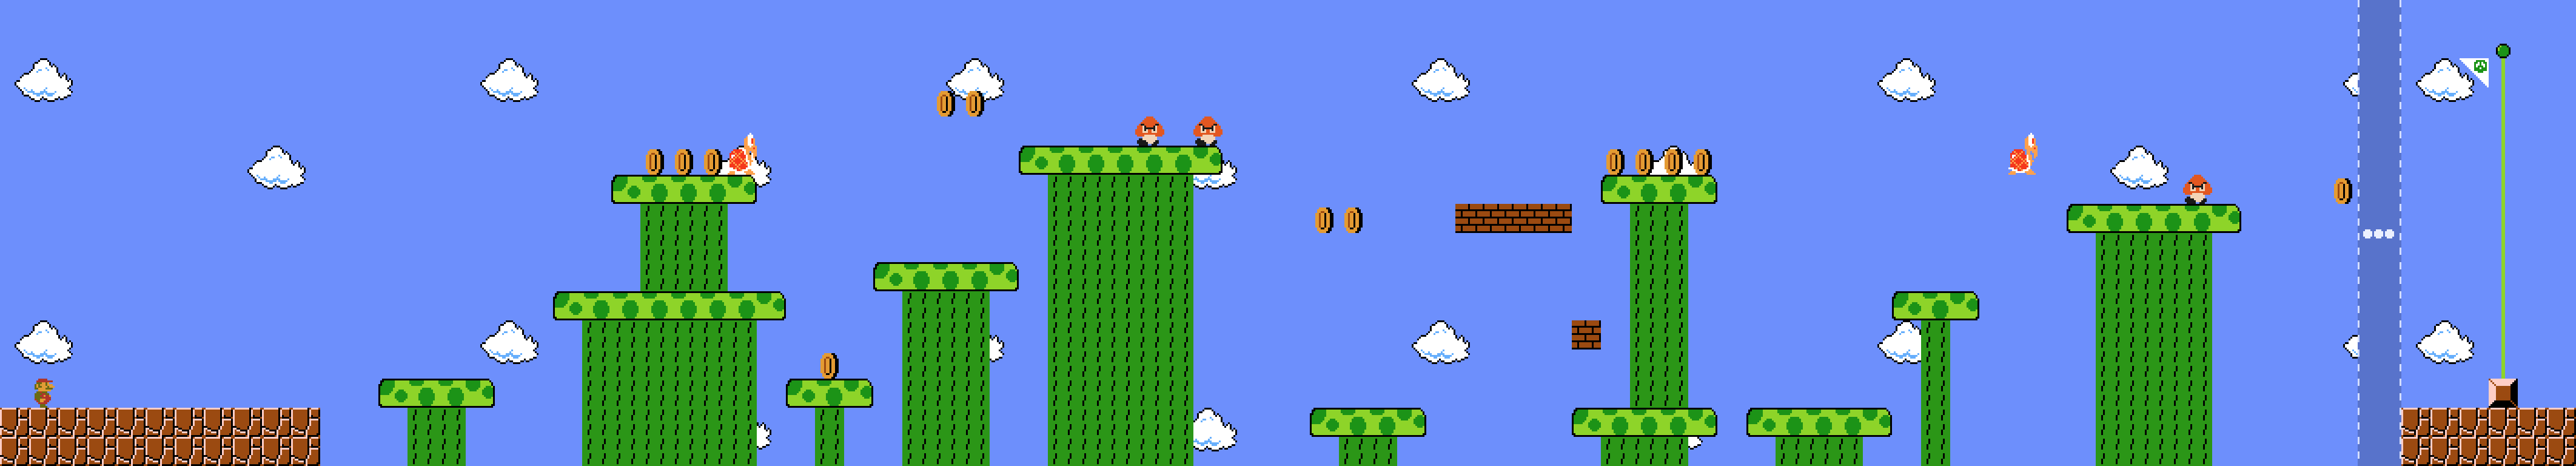
\includegraphics[width=\textwidth]{ascii-level-rendered.png}
\caption{Rendered view of the same segment.}
\end{subfigure}

\caption{Original Super Mario Bros Level (World~1-1 segment).
         \texttt{M} marks Mario's spawn; \texttt{X} is solid ground; \texttt{U} and \texttt{S}
         are question blocks; \texttt{g} is a Goomba;
         \texttt{F} denotes level exit; \texttt{-} is empty air.}
\label{fig:ascii-level}
\end{figure}

\subsection{Level Validation}
\label{subsec:sd-level-validation}

Every submitted level undergoes format validation before insertion into the database. The
validation procedure, implemented in the backend's \texttt{seed.py} module, checks:

\begin{enumerate}
    \item \textbf{Height bounds:} the number of rows must satisfy
          $10 \leq h \leq 20$.
    \item \textbf{Width bounds:} the number of columns must satisfy
          $150 \leq w \leq 250$.  In practice, all submitted generators produce levels
          with widths between 150 and 208 columns; the lower bound of 150
          corresponds to the standard screen width of the original Super Mario Bros.
    \item \textbf{Rectangular shape:} all rows must have identical length.
    \item \textbf{Character whitelist:} every character must belong to the set of
          37 allowed tiles (Table \ref{tab:tile-legend}).
\end{enumerate}

Levels that fail any check are rejected with a descriptive error message. The
platform performs \emph{format-level} validation only, without automated playability
or reachability analysis (e.g.\ checking that the exit is reachable from the spawn).
Content hashes are computed for deduplication.

\section{Battle and Voting System}
\label{sec:sd-battle}

The core user experience is the \emph{battle}: a blind A/B test in which the player
compares two levels produced by different generators, not knowing which generator
produced which level.

\subsection{Battle Flow}
\label{subsec:sd-battle-flow}

A battle proceeds through five stages:

\begin{enumerate}
    \item \textbf{Battle request.} The frontend calls \texttt{POST /v1/battles:next}.
    \item \textbf{Matchmaking.} The AGIS algorithm (Section \ref{sec:sd-matchmaking})
          selects two generators; one random level is drawn from each.
    \item \textbf{Gameplay.} The player plays both levels sequentially (labelled ``Left''
          and ``Right''). During play, the engine records a trajectory of Mario's position
          and death events.
    \item \textbf{Voting.} After completing both levels, the player chooses one of four
          options: \emph{Left is Better}, \emph{Right is Better}, \emph{Tie}, or
          \emph{Skip}. The ``Skip'' option, used when the player feels unable to judge or
          encounters a technical issue, does not affect ratings.
    \item \textbf{Rating update.} The backend updates Glicko-2 ratings for both generators
          atomically within a database transaction (Section \ref{sec:sd-rating}).
\end{enumerate}

Figure \ref{fig:gameplay} shows the main gameplay interface. After completing both levels,
the voting panel (Figure \ref{fig:voting}) allows the player to cast their preference and
optionally tag each level.

\begin{figure}[H]
    \centering
    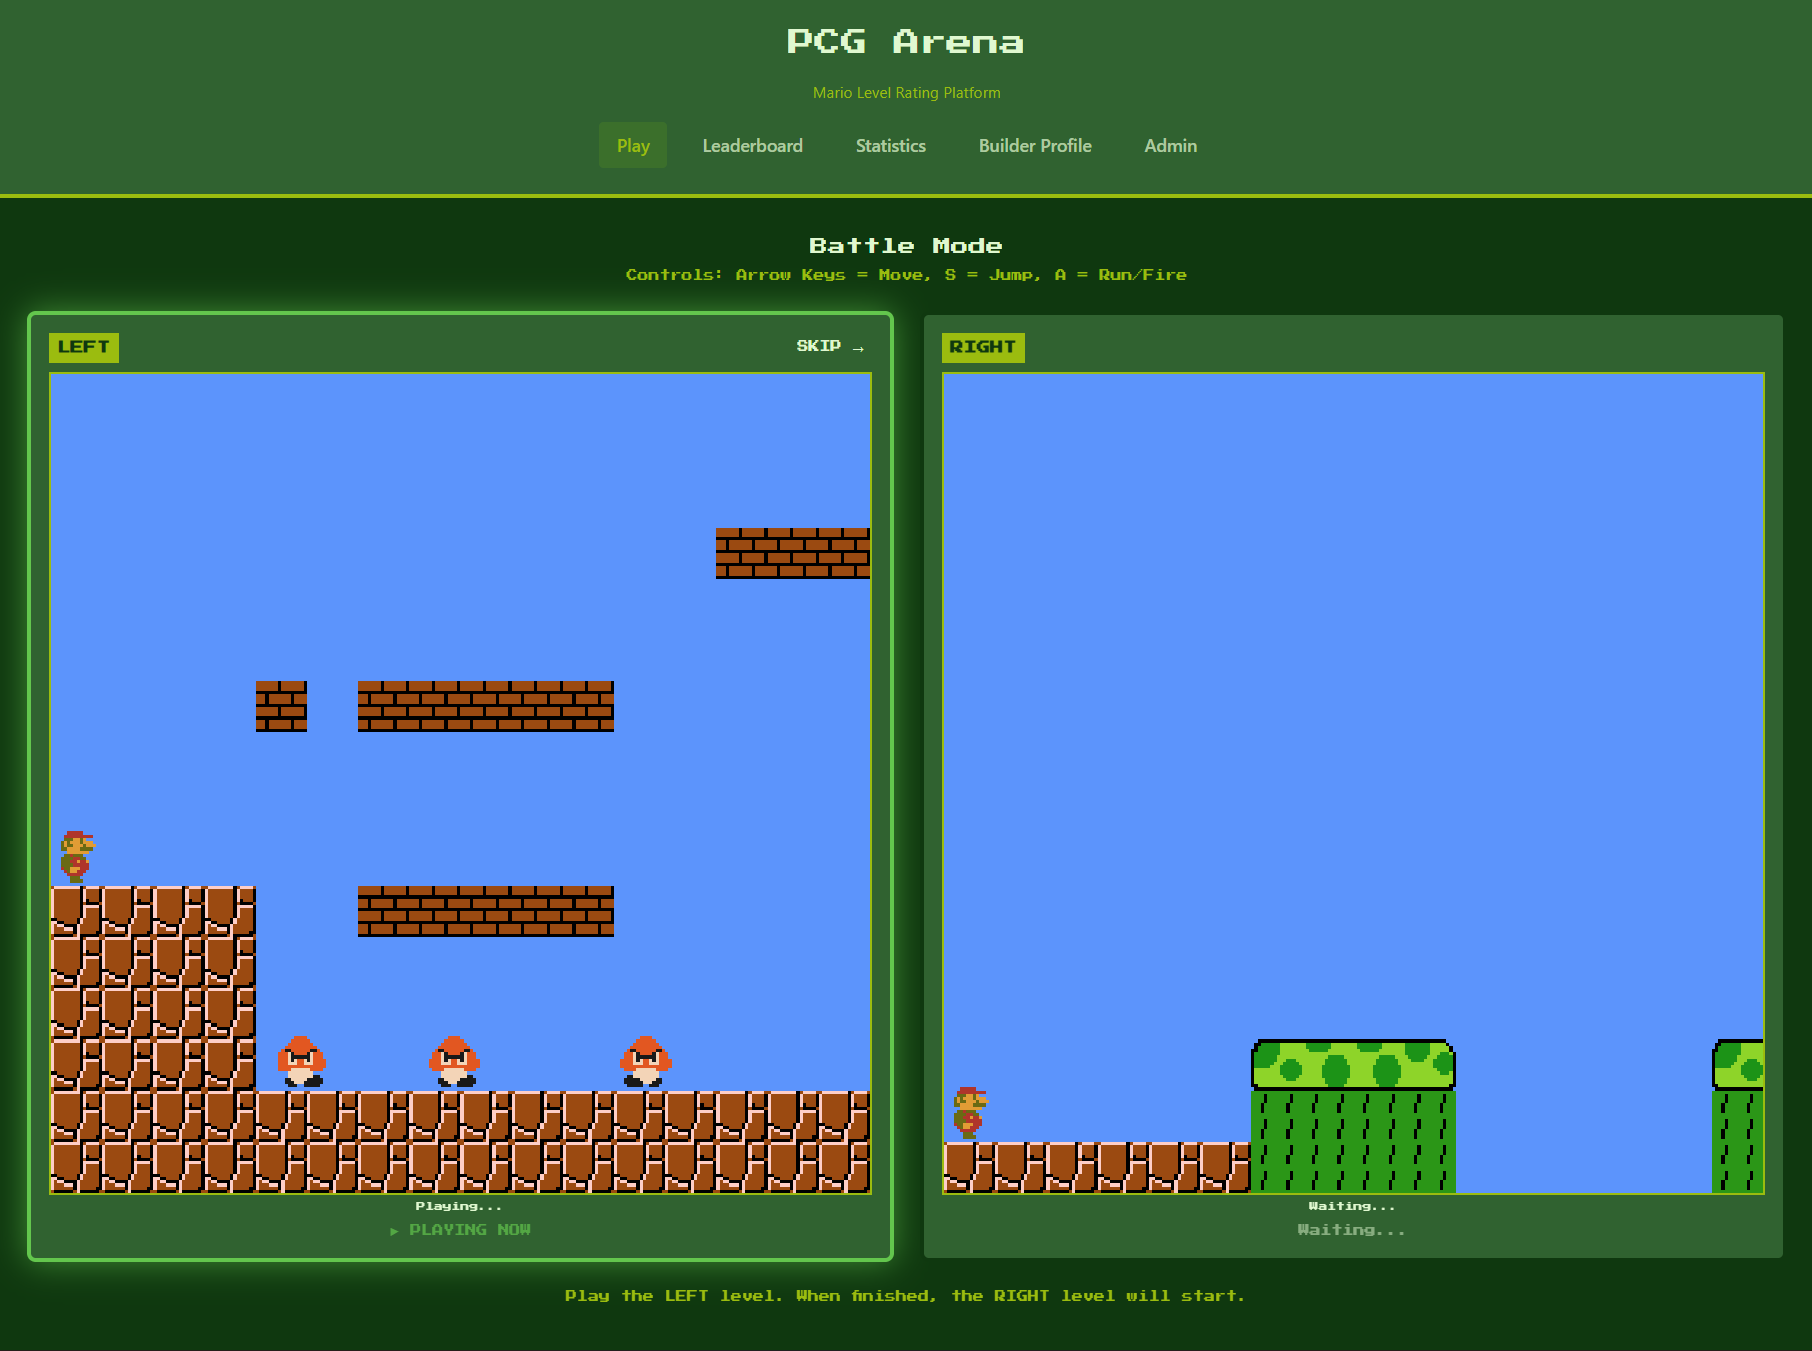
\includegraphics[width=0.95\textwidth]{main_gameplay.png}
    \caption{Main gameplay view: the player experiences a procedurally generated level
             in the browser-based Mario engine.}
    \label{fig:gameplay}
\end{figure}

\begin{figure}[H]
    \centering
    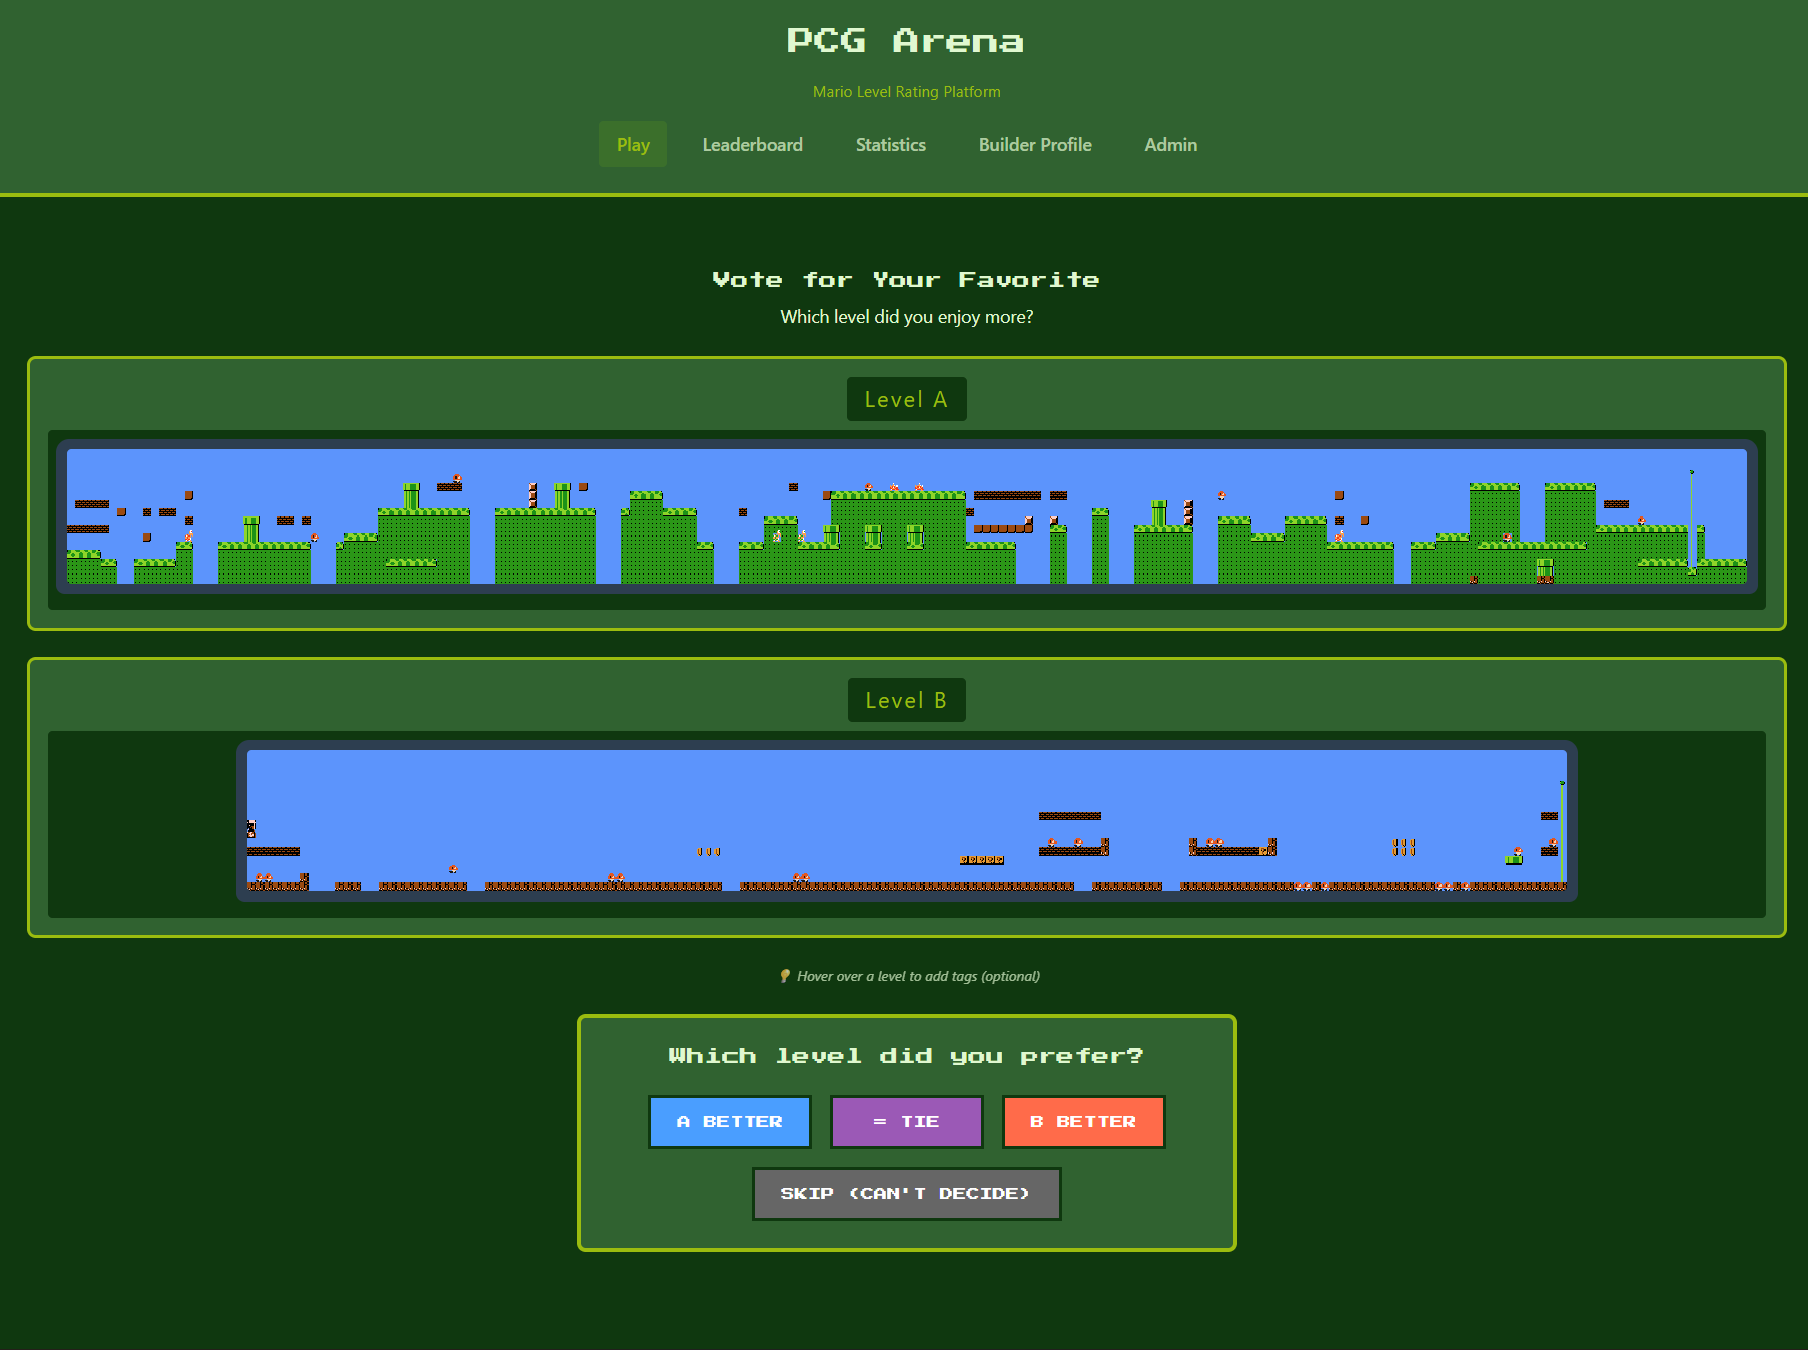
\includegraphics[width=0.90\textwidth]{voting_panel.png}
    \caption{Voting panel shown after both levels are played, with preference buttons.
             Tag selection is accessible by hovering over the level
             (see Figure~\ref{fig:tag-selection}).}
    \label{fig:voting}
\end{figure}

\begin{figure}[H]
    \centering
    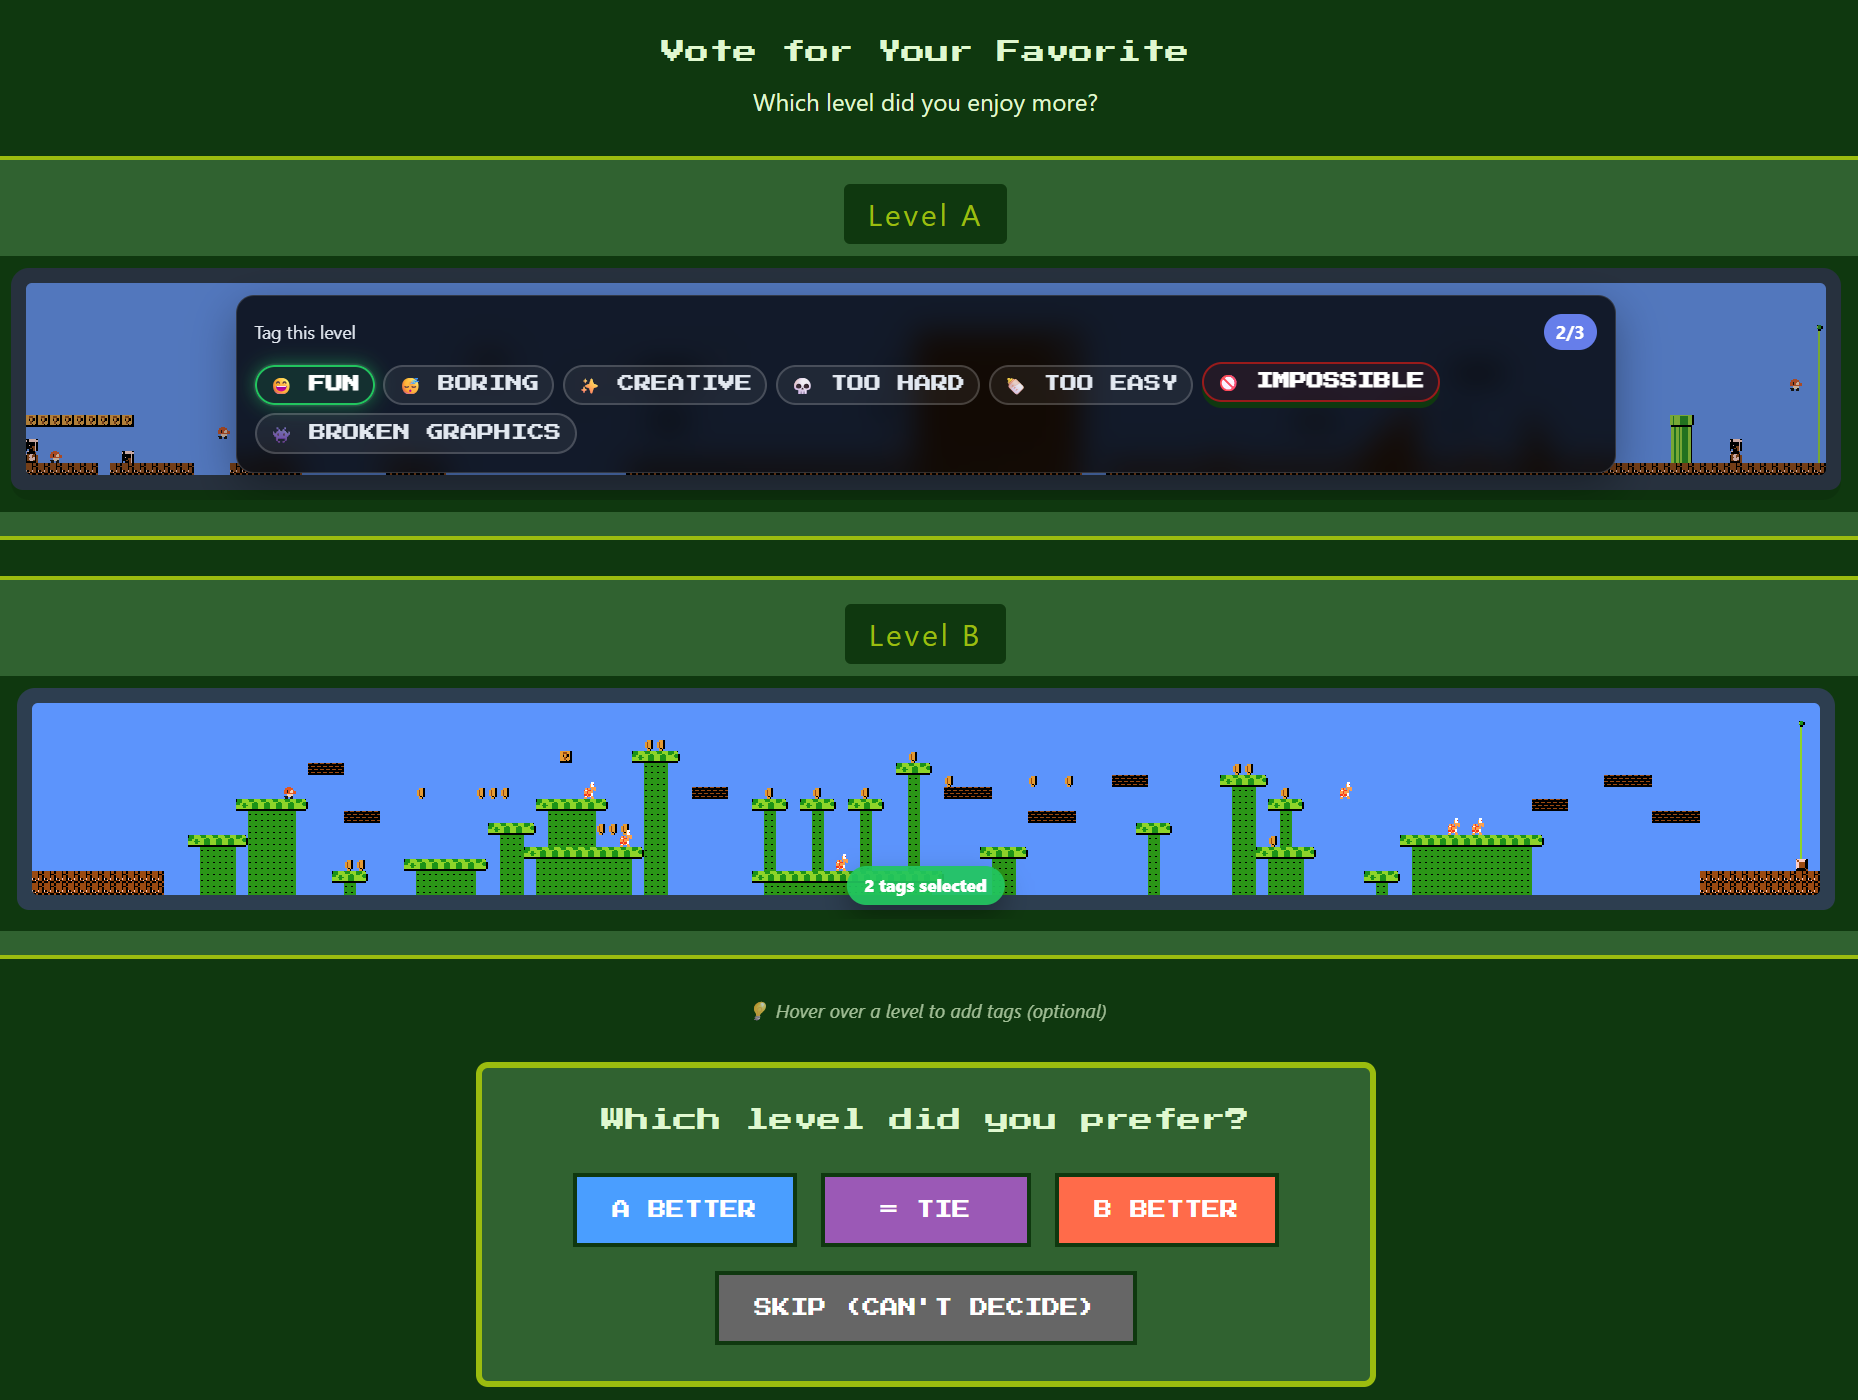
\includegraphics[width=0.90\textwidth]{tag_selection.png}
    \caption{Tag selection popup shown when the player hovers over a level.
             Players may assign up to three descriptive labels per level.}
    \label{fig:tag-selection}
\end{figure}

\subsection{Tagging System}
\label{subsec:sd-tagging}

In addition to the preference vote, players may optionally tag each level in the battle
with up to three descriptive labels drawn from a fixed vocabulary of seven tags
(Table~\ref{tab:tags}), chosen to cover enjoyment, engagement, creativity, difficulty,
playability, and visual correctness.

\begin{table}[H]
\centering
\begin{tabular}{ll}
\toprule
\textbf{Tag} & \textbf{Description} \\
\midrule
\texttt{fun}              & The level was enjoyable to play \\
\texttt{boring}           & The level lacked engagement \\
\texttt{creative}         & The level showed novel or interesting design \\
\texttt{too\_hard}        & The level was excessively difficult \\
\texttt{too\_easy}        & The level was trivially easy \\
\texttt{impossible}       & The level appeared to be uncompletable \\
\texttt{broken\_graphics} & The level had visual or rendering issues \\
\bottomrule
\end{tabular}
\caption{The seven available tags for level characterisation.}
\label{tab:tags}
\end{table}

Tags are stored as boolean columns in the \texttt{votes} table and aggregated in
\texttt{level\_stats} for downstream analysis (Section~\ref{sec:eda-tag-semantics}).

\section{Matchmaking: AGIS Algorithm}
\label{sec:sd-matchmaking}

\subsection{Problem Definition}
\label{subsec:sd-matchmaking-problem}

Given $n$ generators with current Glicko-2 ratings and uncertainties, the matchmaking
problem is to select a pair for the next battle that maximises information gain toward
accurate final rankings. Naive strategies are suboptimal:

\begin{itemize}
    \item \textbf{Uniform random} wastes battles on already-converged pairs.
    \item \textbf{Most-uncertain-first} neglects head-to-head comparisons between
          similarly rated generators.
    \item \textbf{Round-robin} ignores rating information and pairs dissimilar generators.
\end{itemize}

To address these shortcomings, we designed \emph{AGIS} (Adaptive Glicko-Informed
Selection), a two-stage matchmaking algorithm that combines rating
uncertainty, skill similarity, and pairwise coverage into generator selection.
Its components adapt standard ideas from information-theoretic
experimental design (uncertainty sampling and coverage balancing) into a lightweight, Glicko-2-aware matchmaker for PCG evaluation.

\subsection{Stage 1: First Generator Selection}
\label{subsec:sd-agis-stage1}

Each generator $i$ receives a selection weight $w_i$ composing an uncertainty term and
a games-played term:

\begin{equation}
\label{eq:agis-w1}
w_i = \bigl(1 + \widetilde{\text{RD}}_i\bigr)^2 \;\cdot\; \text{boost}(\text{games}_i)
\end{equation}

where $\widetilde{\text{RD}}_i = (\text{RD}_i - \text{RD}_{\min}) / (\text{RD}_{\max} -
\text{RD}_{\min})$ is the normalised rating deviation. The \emph{boost} function provides a $4\times$
weight multiplier for generators with zero games, linearly decaying to $1\times$ at
\texttt{MIN\_GAMES} (default: 30). After convergence, a mild quality bias is applied:

\begin{equation}
\text{boost}_{\text{converged}} = 0.8 + q_{\text{bias}} \cdot
\min\!\Bigl(1,\;\max\!\bigl(0,\;\tfrac{\mu_i - 600}{800}\bigr)\Bigr)
\end{equation}

where $q_{\text{bias}} = 0.2$ is the configurable quality bias strength. The weights
are normalised to sum to 1, forming a categorical (discrete) probability distribution;
the first generator is then drawn from this distribution via weighted random sampling.

\subsection{Stage 2: Second Generator Selection}
\label{subsec:sd-agis-stage2}

The intuition behind Stage 2 is that the most informative battle is one between
generators of \emph{similar} strength (maximising discriminative power) whose ratings
are still \emph{uncertain} (maximising information gain per battle), while ensuring
that every pair accumulates enough head-to-head data for a reliable confusion matrix.
The four weighted components below formalise these intuitions.

Given the first generator $g_1$, the second is selected using a composite pair weight:

\begin{equation}
\label{eq:agis-w2}
w_{1,j} = \alpha \cdot S(g_1, g_j) \;+\; \beta \cdot U(g_j) \;+\;
           \gamma \cdot I(g_1, g_j) \;+\; \text{cov}(g_1, g_j)
\end{equation}

The four components are:

\begin{itemize}
    \item \textbf{Rating similarity} $S(g_1, g_j) = \exp\!\bigl(-\Delta\mu^2 / 2\sigma_s^2\bigr)$,
          a Gaussian kernel with $\sigma_s = 150$ penalising large rating gaps.
    \item \textbf{Uncertainty} $U(g_j) = 1 + \widetilde{\text{RD}}_j$, favouring
          uncertain generators (range $[1, 2]$).
    \item \textbf{Information gain} $I(g_1, g_j)$, incorporating the joint RD
          and a match-quality estimate.
    \item \textbf{Coverage bonus} $\text{cov}(g_1, g_j)$: for pairs with fewer than
          \texttt{TARGET\_BATTLES\_PER\_PAIR} (default: 10) battles, an exponential
          bonus $2 \cdot e^{-c/3}$ is applied, where $c$ is the current battle count;
          otherwise a residual $0.1$ is used.
\end{itemize}

\subsection{Parameters}
\label{subsec:sd-agis-params}

Table \ref{tab:agis-params} lists the configurable AGIS parameters and their defaults,
which are set via environment variables.

\begin{table}[H]
\centering
\begin{tabular}{llr}
\toprule
\textbf{Parameter} & \textbf{Description} & \textbf{Default} \\
\midrule
$\alpha$ & Rating similarity weight & 0.5 \\
$\beta$  & Uncertainty weight       & 0.3 \\
$\gamma$ & Information gain weight  & 0.2 \\
\texttt{MIN\_GAMES}            & Games before ``converged''  & 30 \\
\texttt{TARGET\_BATTLES\_PER\_PAIR} & Min.\ battles per pair & 10 \\
\texttt{RATING\_SIGMA}        & Similarity kernel $\sigma_s$ & 150.0 \\
\texttt{QUALITY\_BIAS}        & Quality bias strength $q_{\text{bias}}$ & 0.2 \\
\bottomrule
\end{tabular}
\caption{AGIS algorithm parameters and default values.}
\label{tab:agis-params}
\end{table}

\section{Glicko-2 Rating System}
\label{sec:sd-rating}

PCG Arena uses the Glicko-2 rating system \cite{glickman2012glicko2} to maintain
uncertainty-aware rankings. Each generator carries three parameters:

\begin{itemize}
    \item \textbf{Rating ($\mu$):} the skill estimate, displayed on a scale centred at 1000.
    \item \textbf{Rating Deviation (RD, $\phi$):} the uncertainty in the rating. High RD
          indicates an unreliable estimate; low RD indicates a well-established rating.
    \item \textbf{Volatility ($\sigma$):} the expected fluctuation in performance over time.
\end{itemize}

The mathematical foundations of the Glicko-2 system (the Bradley-Terry
model, expected score computation, and the update equations for $\phi'$ and
$\mu'$) are presented in Section~\ref{subsec:bg-glicko2}. Here we describe the
implementation-specific aspects of how PCG Arena applies these formulas.

\subsection{Rating Update Procedure}
\label{subsec:sd-glicko-update}

After each battle, the winning generator receives a score of 1, the loser 0, and ties
yield 0.5 for both. Using the expected score and update equations from
Section~\ref{subsec:bg-glicko2}, the implementation proceeds as follows:

\begin{enumerate}
    \item Convert ratings to the internal Glicko-2 scale (centred at 0, divided by
          $\lambda = 173.7178$).  This constant equals $400 / \ln 10 \approx 173.7178$
          and bridges the Elo convention (400 points per tenfold win-probability change)
          with the natural logistic function used internally by Glicko-2.
    \item Compute the variance $v$ from the opponent's RD.
    \item Compute $\Delta = v \cdot g(\phi_B)(s - E)$, where $s$ is the actual score.
    \item Update volatility $\sigma'$ via the iterative Illinois algorithm
          (system constant $\tau = 0.5$).
    \item Update RD and rating using Equations~\ref{eq:glicko-rd-bg}--\ref{eq:glicko-mu-bg}.
    \item Convert back to the display scale and clamp to $[100, 3000]$.
\end{enumerate}

All rating updates are performed atomically within a single database transaction, with
an audit record written to the \texttt{rating\_events} table.

\subsection{Configuration}
\label{subsec:sd-glicko-config}

Table \ref{tab:glicko-params} lists the Glicko-2 constants used by PCG Arena.

\begin{table}[H]
\centering
\begin{tabular}{lr}
\toprule
\textbf{Parameter} & \textbf{Value} \\
\midrule
Initial rating ($\mu_0$)       & 1000 \\
Initial RD ($\phi_0$)          & 350 \\
Initial volatility ($\sigma_0$) & 0.06 \\
System constant ($\tau$)       & 0.5 \\
Scale factor ($\lambda$)       & 173.7178 \\
Minimum RD                     & 30 \\
Maximum RD                     & 350 \\
Minimum rating                 & 100 \\
Maximum rating                 & 3000 \\
\bottomrule
\end{tabular}
\caption{Glicko-2 configuration parameters.}
\label{tab:glicko-params}
\end{table}

The RD of each generator provides a natural 95\% confidence interval for its true rating:
$\text{CI}_{95\%} = [\mu - 1.96\,\text{RD},\;\mu + 1.96\,\text{RD}]$.
However, the public leaderboard displays only the point-estimate rating; confidence
intervals are not shown on the platform's frontend.
Figure \ref{fig:leaderboard} shows the leaderboard as seen by players.

\begin{figure}[H]
    \centering
    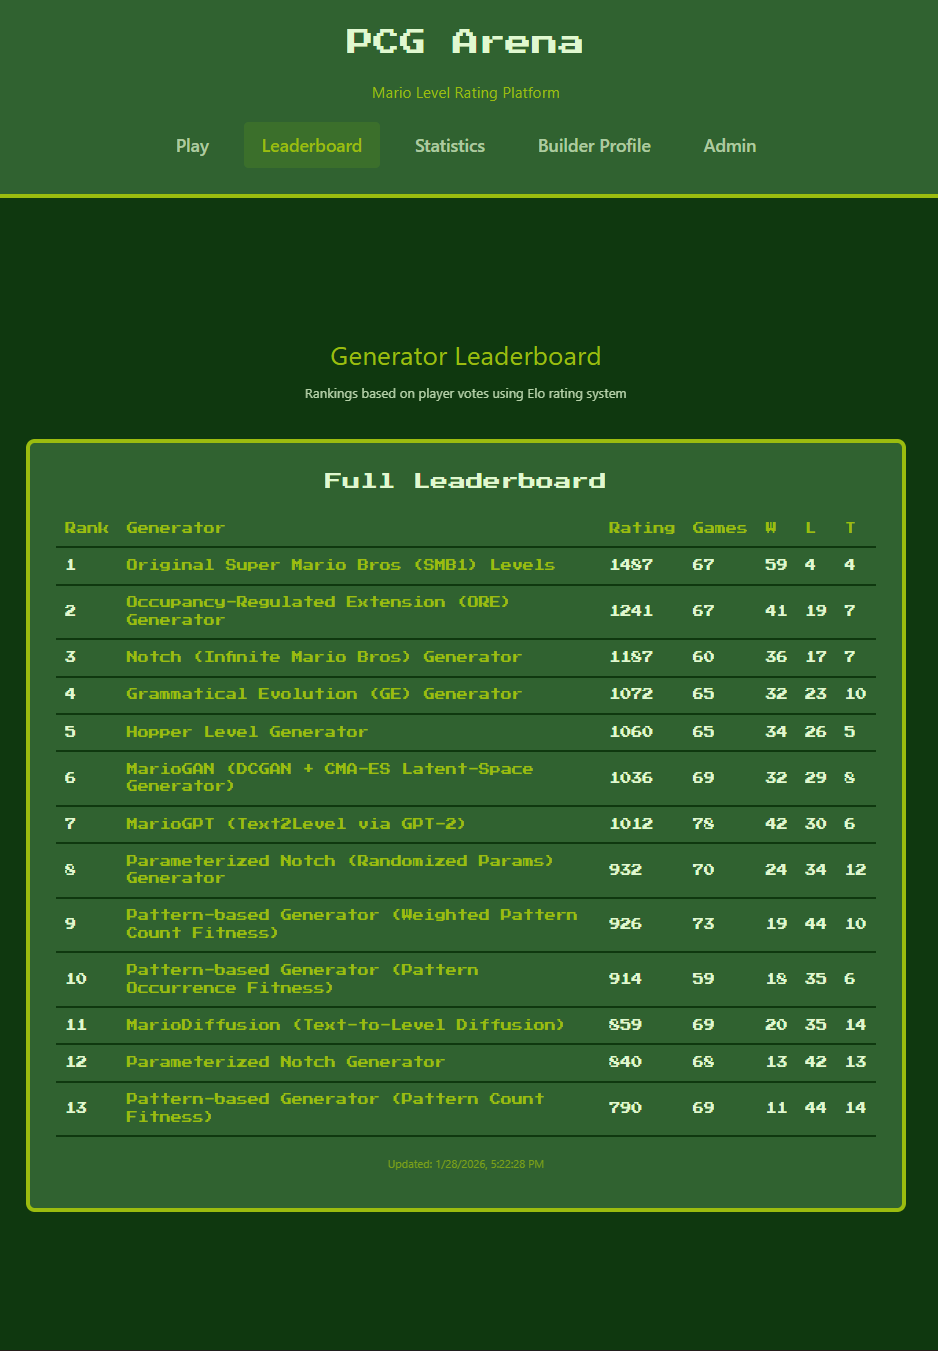
\includegraphics[width=0.95\textwidth]{leaderboard.png}
    \caption{Public leaderboard ranking generators by their Glicko-2 rating.}
    \label{fig:leaderboard}
\end{figure}

Clicking a generator reveals detailed statistics including rating history, per-opponent
win rates, a level gallery, and tag distributions
(Figure \ref{fig:generator-preview}).

\begin{figure}[H]
    \centering
    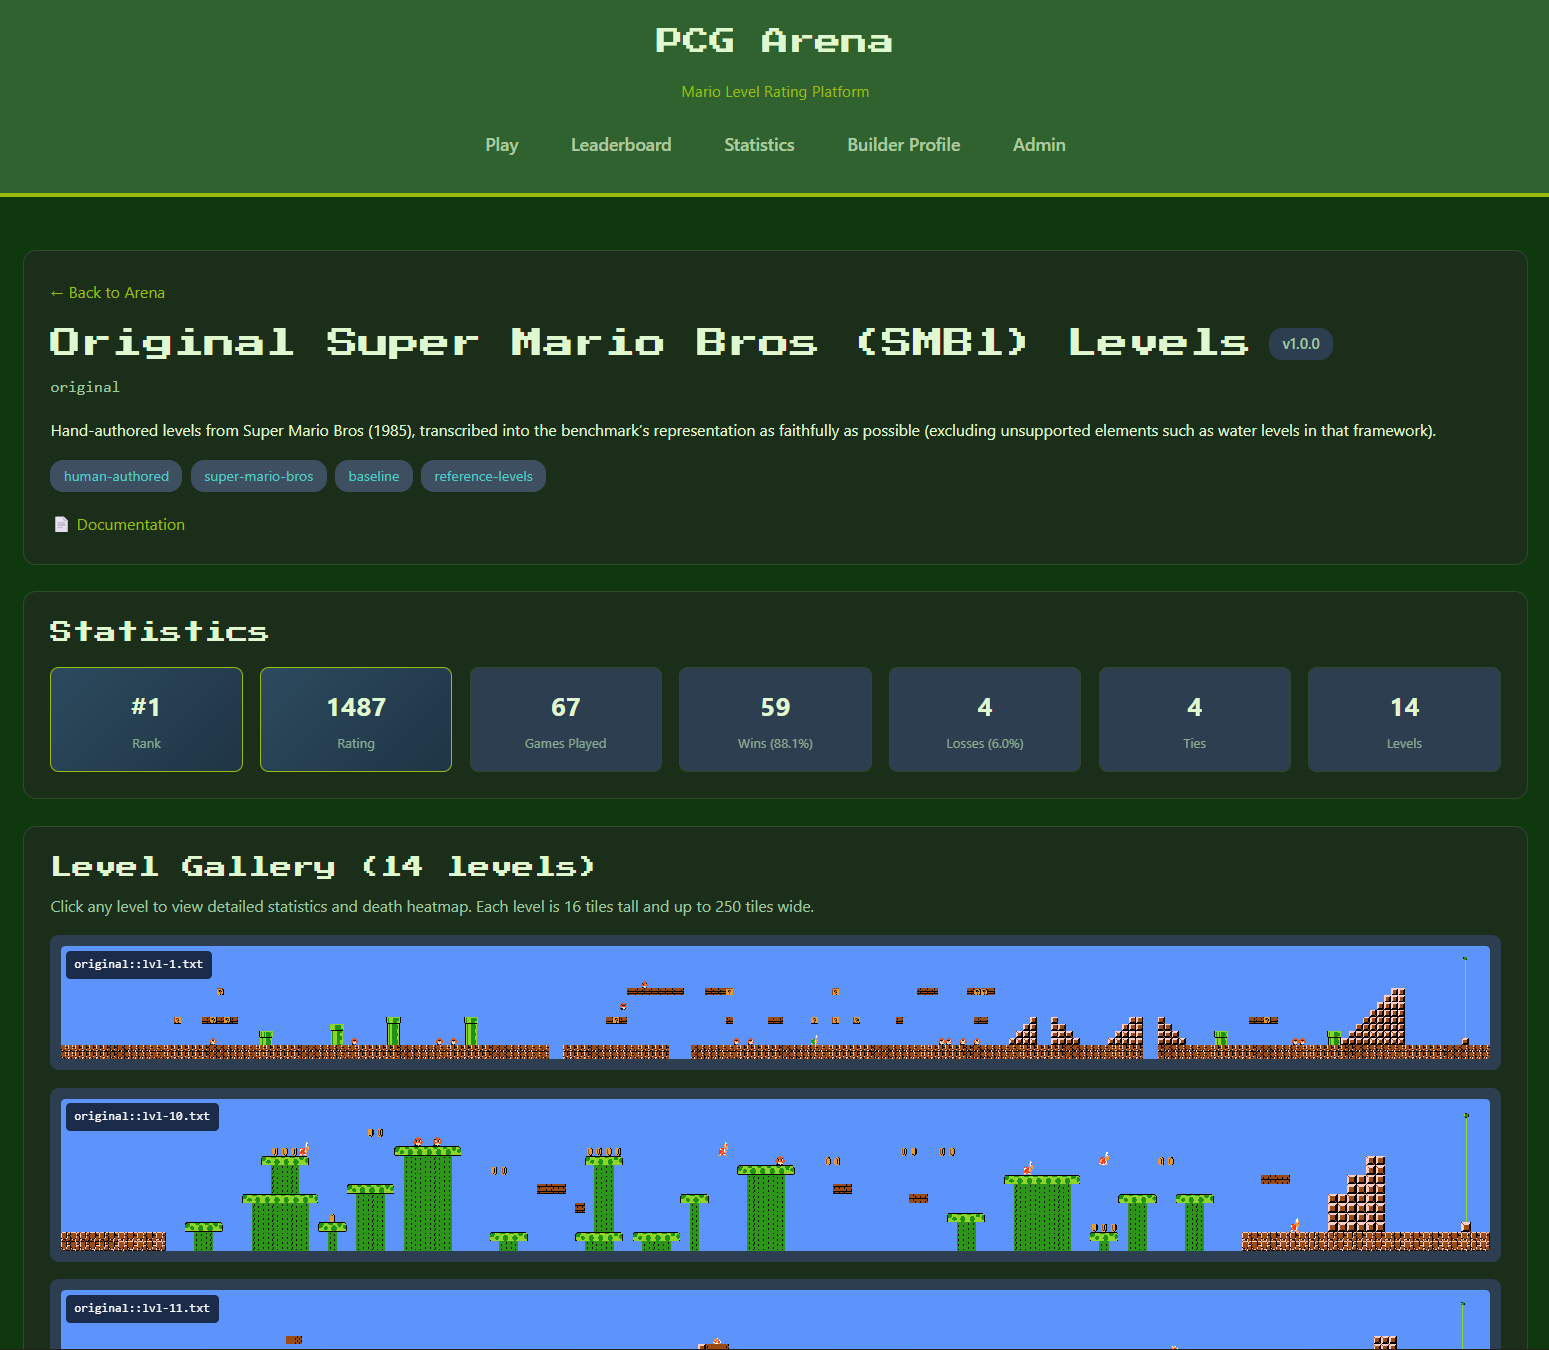
\includegraphics[width=0.95\textwidth]{generator_preview.png}
    \caption{Generator detail page showing level gallery and performance statistics.}
    \label{fig:generator-preview}
\end{figure}

For researchers, the platform also exposes a per-level
analytics view (Figure~\ref{fig:eda-detailed-level-stats}) that overlays the
level map with recorded player traces, death locations, and tag counts.

\begin{figure}[H]
\centering
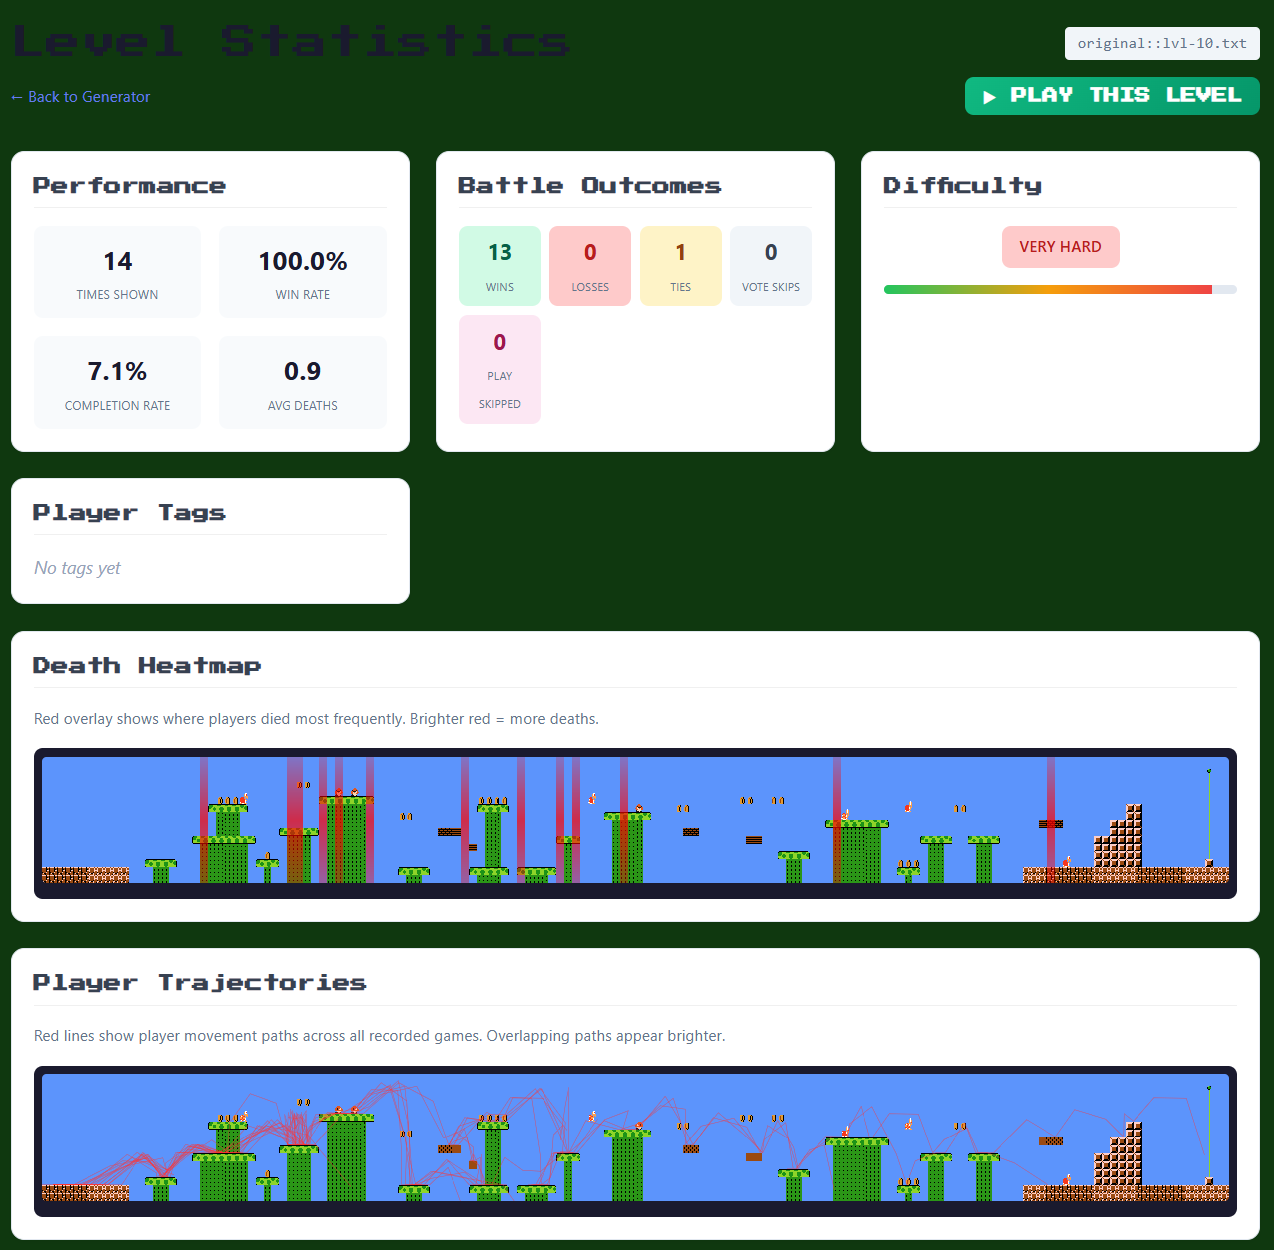
\includegraphics[width=0.95\textwidth]{detailed_level_statistics_page.png}
\caption{Detailed Level Statistics page from PCG Arena. The interface supports qualitative inspection of individual levels through trajectory overlays, death locations, tag counts, and level visualization.}
\label{fig:eda-detailed-level-stats}
\end{figure}

\section{Builder Profile and Generator Submission}
\label{sec:sd-builder}

Authenticated users may submit their own generators through the Builder Profile page.
The submission workflow is:

\begin{enumerate}
    \item The user provides generator metadata: name, version, description, and a URL to
          the generator's source repository.
    \item The user uploads a ZIP archive containing level files in the ASCII tilemap format.
    \item The backend validates every level (Section \ref{subsec:sd-level-validation}).
          Levels that fail validation are rejected with detailed error messages.
    \item Valid levels and the generator record are inserted into the database.
    \item An initial Glicko-2 rating of $1000 \pm 350$ is assigned.
    \item The generator appears on the leaderboard immediately and enters the matchmaking
          pool.
\end{enumerate}

Each user may own at most three generators.
When a user wishes to remove a generator, the system distinguishes two cases.  If the
generator has already participated in battles, it is \emph{soft-deleted}: marked as
inactive and excluded from future matchmaking, but its records (levels, ratings, votes)
are retained so that historical analyses and the confusion matrix remain consistent.
If the generator has never appeared in a battle, it is \emph{hard-deleted} (fully
removed from the database) since no other data depends on it.

Figure \ref{fig:builder} shows the Builder Profile page.

\begin{figure}[H]
    \centering
    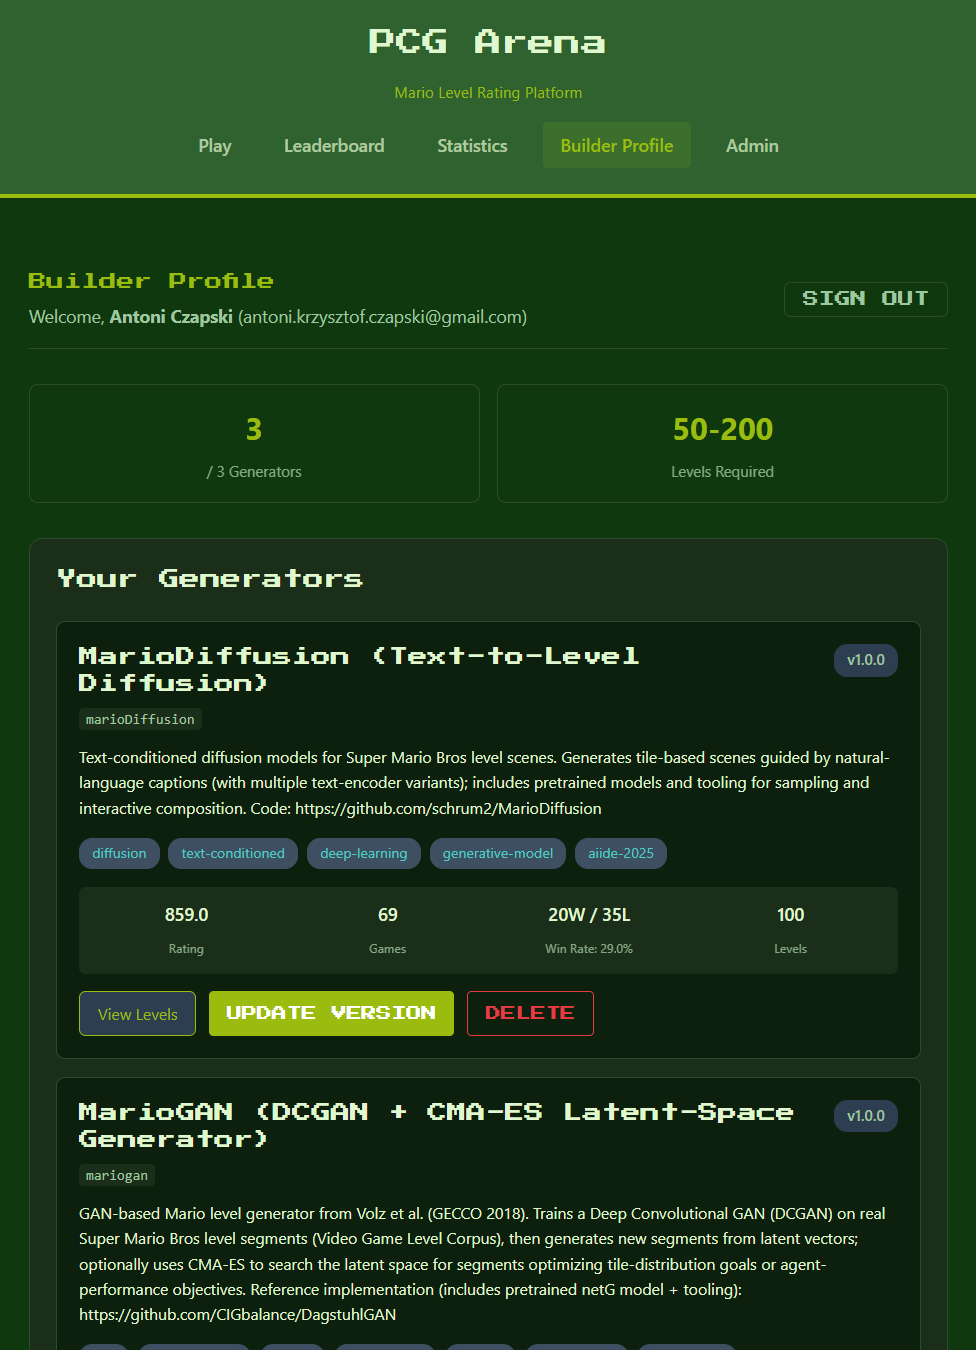
\includegraphics[width=0.95\textwidth]{builder_profile.png}
    \caption{Builder Profile page for submitting and managing generators.}
    \label{fig:builder}
\end{figure}

\section{Authentication}
\label{sec:sd-auth}

PCG Arena supports two authentication methods:

\begin{itemize}
    \item \textbf{Google OAuth 2.0.} The frontend opens a Google sign-in popup; the
          returned ID token (JWT) is sent to \texttt{POST /v1/auth/google}, where the
          backend verifies it against Google's servers. Google users are automatically
          marked as email-verified.
    \item \textbf{Email and password.} Users register with an email, password, and display
          name. Passwords are hashed with bcrypt (work factor 12). A verification email
          is sent via Twilio SendGrid containing a unique token (64 hex characters,
          24-hour expiry).
\end{itemize}

Upon successful authentication, the backend issues a session cookie
(\texttt{arena\_session}) containing a 256-bit cryptographically random token. Sessions
expire after seven days. HTTP-only cookies prevent client-side script access.

Administrative access is granted to users whose email addresses appear in the
\texttt{ARENA\_ADMIN\_EMAILS} configuration list.

\section{Deployment and Infrastructure}
\label{sec:sd-deployment}

PCG Arena is deployed on Google Cloud Platform using a single Compute Engine instance
(\texttt{e2-micro}, Ubuntu 22.04 LTS). The backend runs inside a Docker container
orchestrated by \texttt{docker-compose}, with the SQLite database file bind-mounted
from the host for persistence across container rebuilds.

\noindent
Caddy acts as the reverse proxy and handles:

\begin{itemize}[nosep]
    \item Automatic TLS certificate provisioning and renewal (Let's Encrypt).
    \item HTTP-to-HTTPS redirection.
    \item Reverse proxying API requests to \texttt{localhost:8080}.
    \item Static file serving for the frontend production build.
\end{itemize}

The platform is accessible at \texttt{https://pcg-arena.com}. The backend binds to
\texttt{127.0.0.1:8080} and is not exposed to the public internet directly; all external
traffic passes through Caddy. Firewall rules allow only ports 80 and 443. Database backups
are performed via a scheduled script that copies the SQLite file to a timestamped archive.




\chapter{User Study --- Measuring Player Preference}
\label{ch:eda}

This chapter analyses the PCG Arena data as a user study of player
preference. Section~\ref{sec:eda-study-design} describes the study protocol,
the dataset, and the data-collection timeline. Next, to address RQ1,
Section~\ref{sec:eda-rankings} derives a
preference ranking of generators from blind pairwise votes, and
Section~\ref{sec:eda-user-heterogeneity} examines whether the anonymous player
population is consistent enough for this aggregation to be meaningful. To address RQ2,
Sections~\ref{sec:eda-static-expressive-range}--\ref{sec:eda-tag-semantics}
test whether static level structure, gameplay trajectories, and descriptive
tags can explain or replace the ranking, and Section~\ref{sec:dpo-judge}
constructs a heuristic judge function that Chapter~\ref{ch:mariodpo} uses to label
additional training pairs.

The analysis is exploratory and relies on patterns observed in the data and its visualisations as the sample size is too small to support strong statistical claims.

% ===================================================================
\section{Study Protocol and Dataset}
\label{sec:eda-study-design}

Participants were recruited through university social-media channels, word of mouth among game-development and computer-science communities, and a small promoted Reddit campaign targeting game-development and procedural-generation communities.\footnote{Recruitment post: \url{https://www.reddit.com/r/proceduralgeneration/s/pmltOkw37q}.} Participation was anonymous: the platform assigned browser-based player and session identifiers persisted through cookies or local browser storage.

The promoted Reddit campaign recorded 62,407 impressions.
Summing the country-level ad exports from 1 January--31 May 2026 gives a reported reach of 55,001
and 415 clicks (Figure~\ref{fig:reddit-recruitment}), reflecting where the recruitment advertisement was shown and clicked.

\begin{figure}[H]
\centering
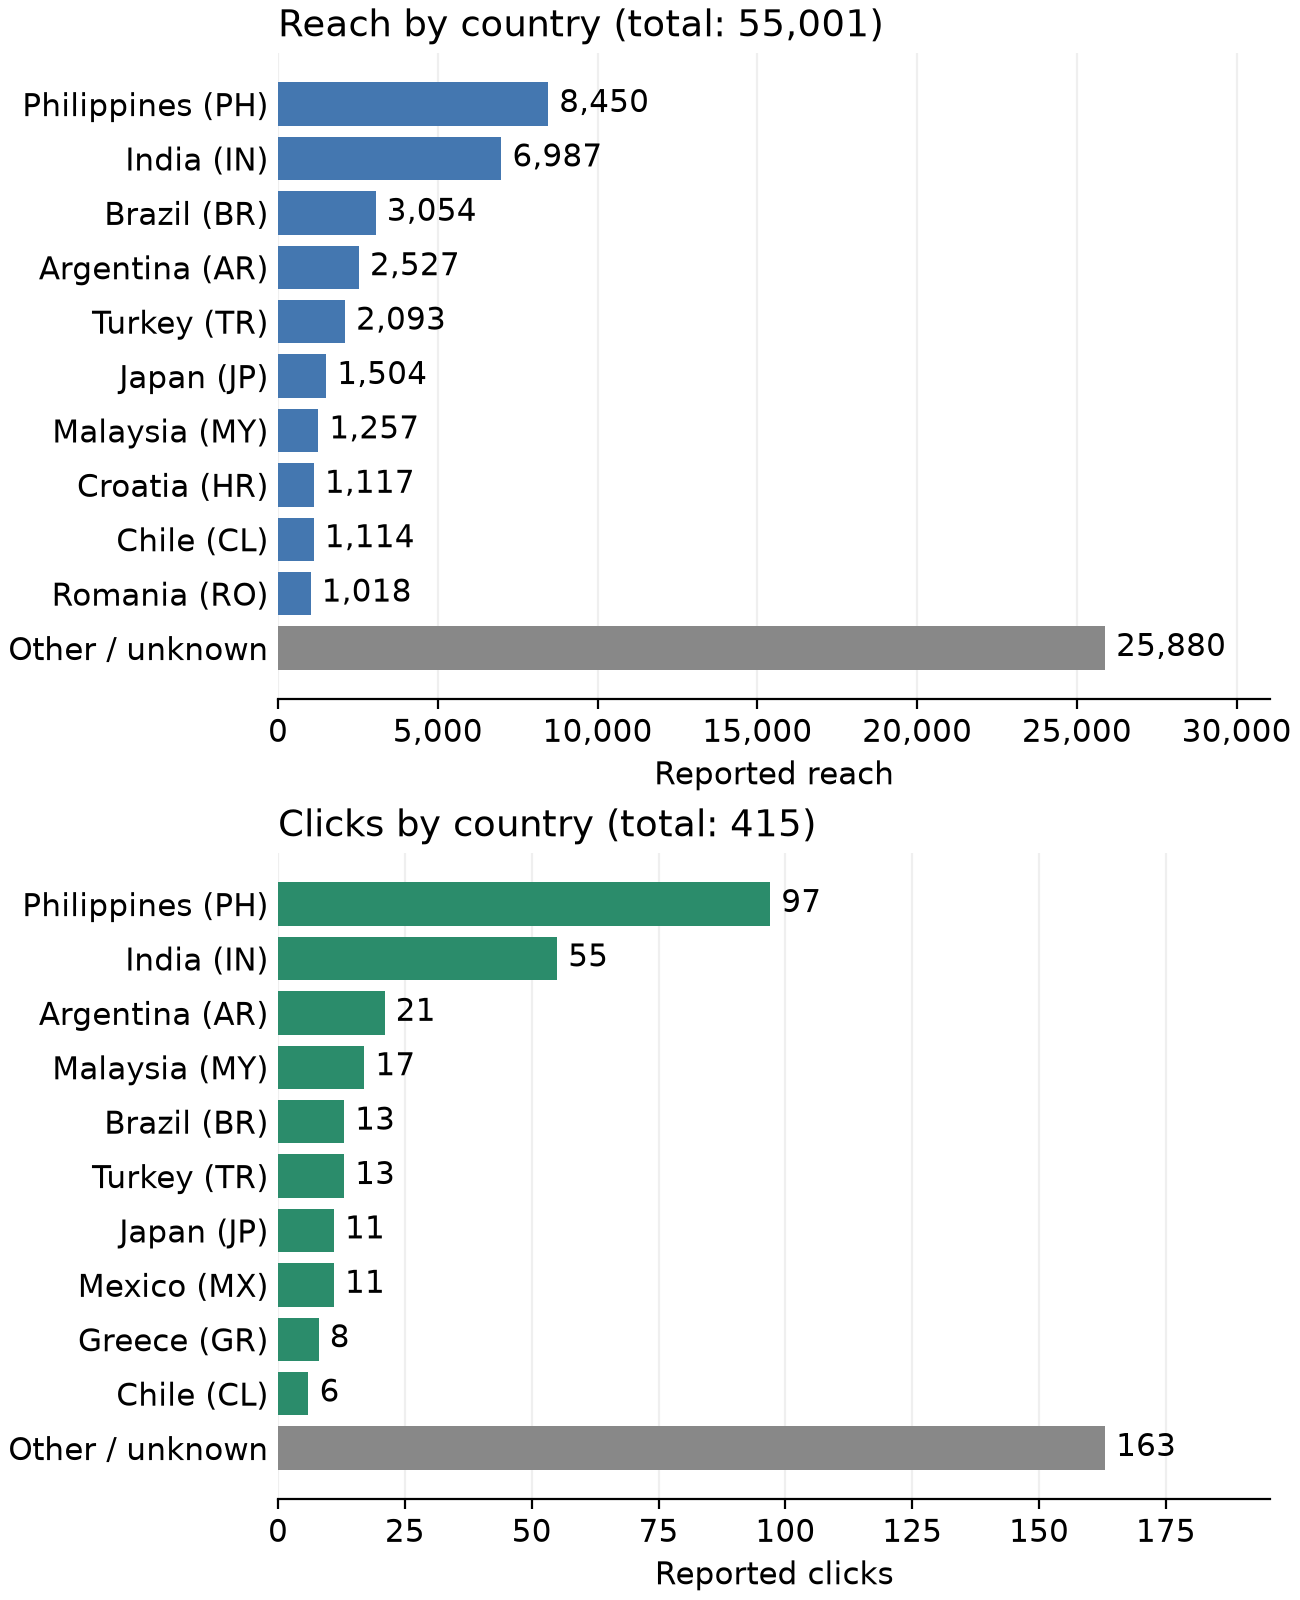
\includegraphics[width=\textwidth]{reddit_recruitment.png}
\caption{Reddit recruitment campaign: reported reach (top) and
click count (bottom) by country from the country-level ad exports for
1 January--31 May 2026. Each panel shows the ten highest-count
countries; the remaining countries and records without a country code
are grouped as ``Other / unknown'' (total reach: 55,001; total clicks: 415).}
\label{fig:reddit-recruitment}
\end{figure}

Each battle used a blind A/B protocol. A player saw two levels from different generators, played one attempt on each side, and then selected the preferred side, a tie, or skip. Optional tags could be attached to either side. Restricting each side to a single attempt was a deliberate design choice: a multi-attempt protocol was also implemented and tested, but single-attempt battles yield substantially more pairwise comparisons per unit of player time.

The May 2026 analysis export contains the data summarized in Table~\ref{tab:eda-dataset}. Skip votes are included in engagement summaries but excluded from preference rankings. Ties are treated as 0.5 points for each side.

\begin{table}[H]
\centering
\caption{Dataset summary for the exploratory analysis.}
\label{tab:eda-dataset}
\begin{tabular}{lr}
\toprule
\textbf{Quantity} & \textbf{Count} \\
\midrule
Vote rows analyzed & 1,000 \\
Anonymous player IDs in vote table & 77 \\
Level-stat records exported & 1,104 \\
Generator IDs & 14 \\
Per-side telemetry records & 2,000 \\
Played side records & 1,968 \\
Embedded trajectory records & 1,968 \\
Tag assignments & 329 \\
\bottomrule
\end{tabular}
\end{table}

Vote outcomes are balanced between the two screen sides (418 left wins and 398 right wins, with 165 ties and 19 skips), and the assignment of levels to the left or right side was randomised. The median play duration per side is 8.0 seconds, with a small number of inactive-tab outliers.

The May 2026 export is the final snapshot of the data-collection process summarised in Table~\ref{tab:eda-timeline}.
MarioDPO (Chapter~\ref{ch:mariodpo}) was trained once on the January 2026 training snapshot and deployed without further changes. The analyses in this chapter use the May export because its larger sample size yields tighter confidence intervals while evaluating the same frozen model and baseline generators.

\begin{table}[H]
\centering
\footnotesize
\begin{tabular}{@{} l l p{2.4cm} p{4.2cm} @{}}
\toprule
\textbf{Phase} & \textbf{Period} & \textbf{Data} & \textbf{Role in this study} \\
\midrule
Baseline collection & launch $\to$ Jan.\ 2026 & votes over the 13 baseline generators & --- \\
Training snapshot & Jan.\ 2026 & 473 usable non-tie votes & judge calibration and DPO training pairs \\
MarioDPO deployment & Jan.\ 2026 & --- & model frozen \\
Full export & May 2026 & 1,000 votes, 14 generators & definitive analysis and generator evaluation \\
\bottomrule
\end{tabular}
\caption{Timeline of PCG Arena data snapshots and their roles.
MarioDPO was trained once on the January 2026 training snapshot and deployed
unchanged; the May export therefore evaluates the same frozen model.}
\label{tab:eda-timeline}
\end{table}

% ===================================================================
\section{Generator Preference Ranking}
\label{sec:eda-rankings}

The primary goal of PCG Arena is to measure human preference between generators. For each non-skip battle, the selected side receives score 1, the rejected side receives score 0, and ties give 0.5 to both sides. Figure~\ref{fig:eda-generator-ranking} shows the resulting generator leaderboard with 95\% bootstrap confidence intervals over votes.

\begin{figure}[H]
\centering
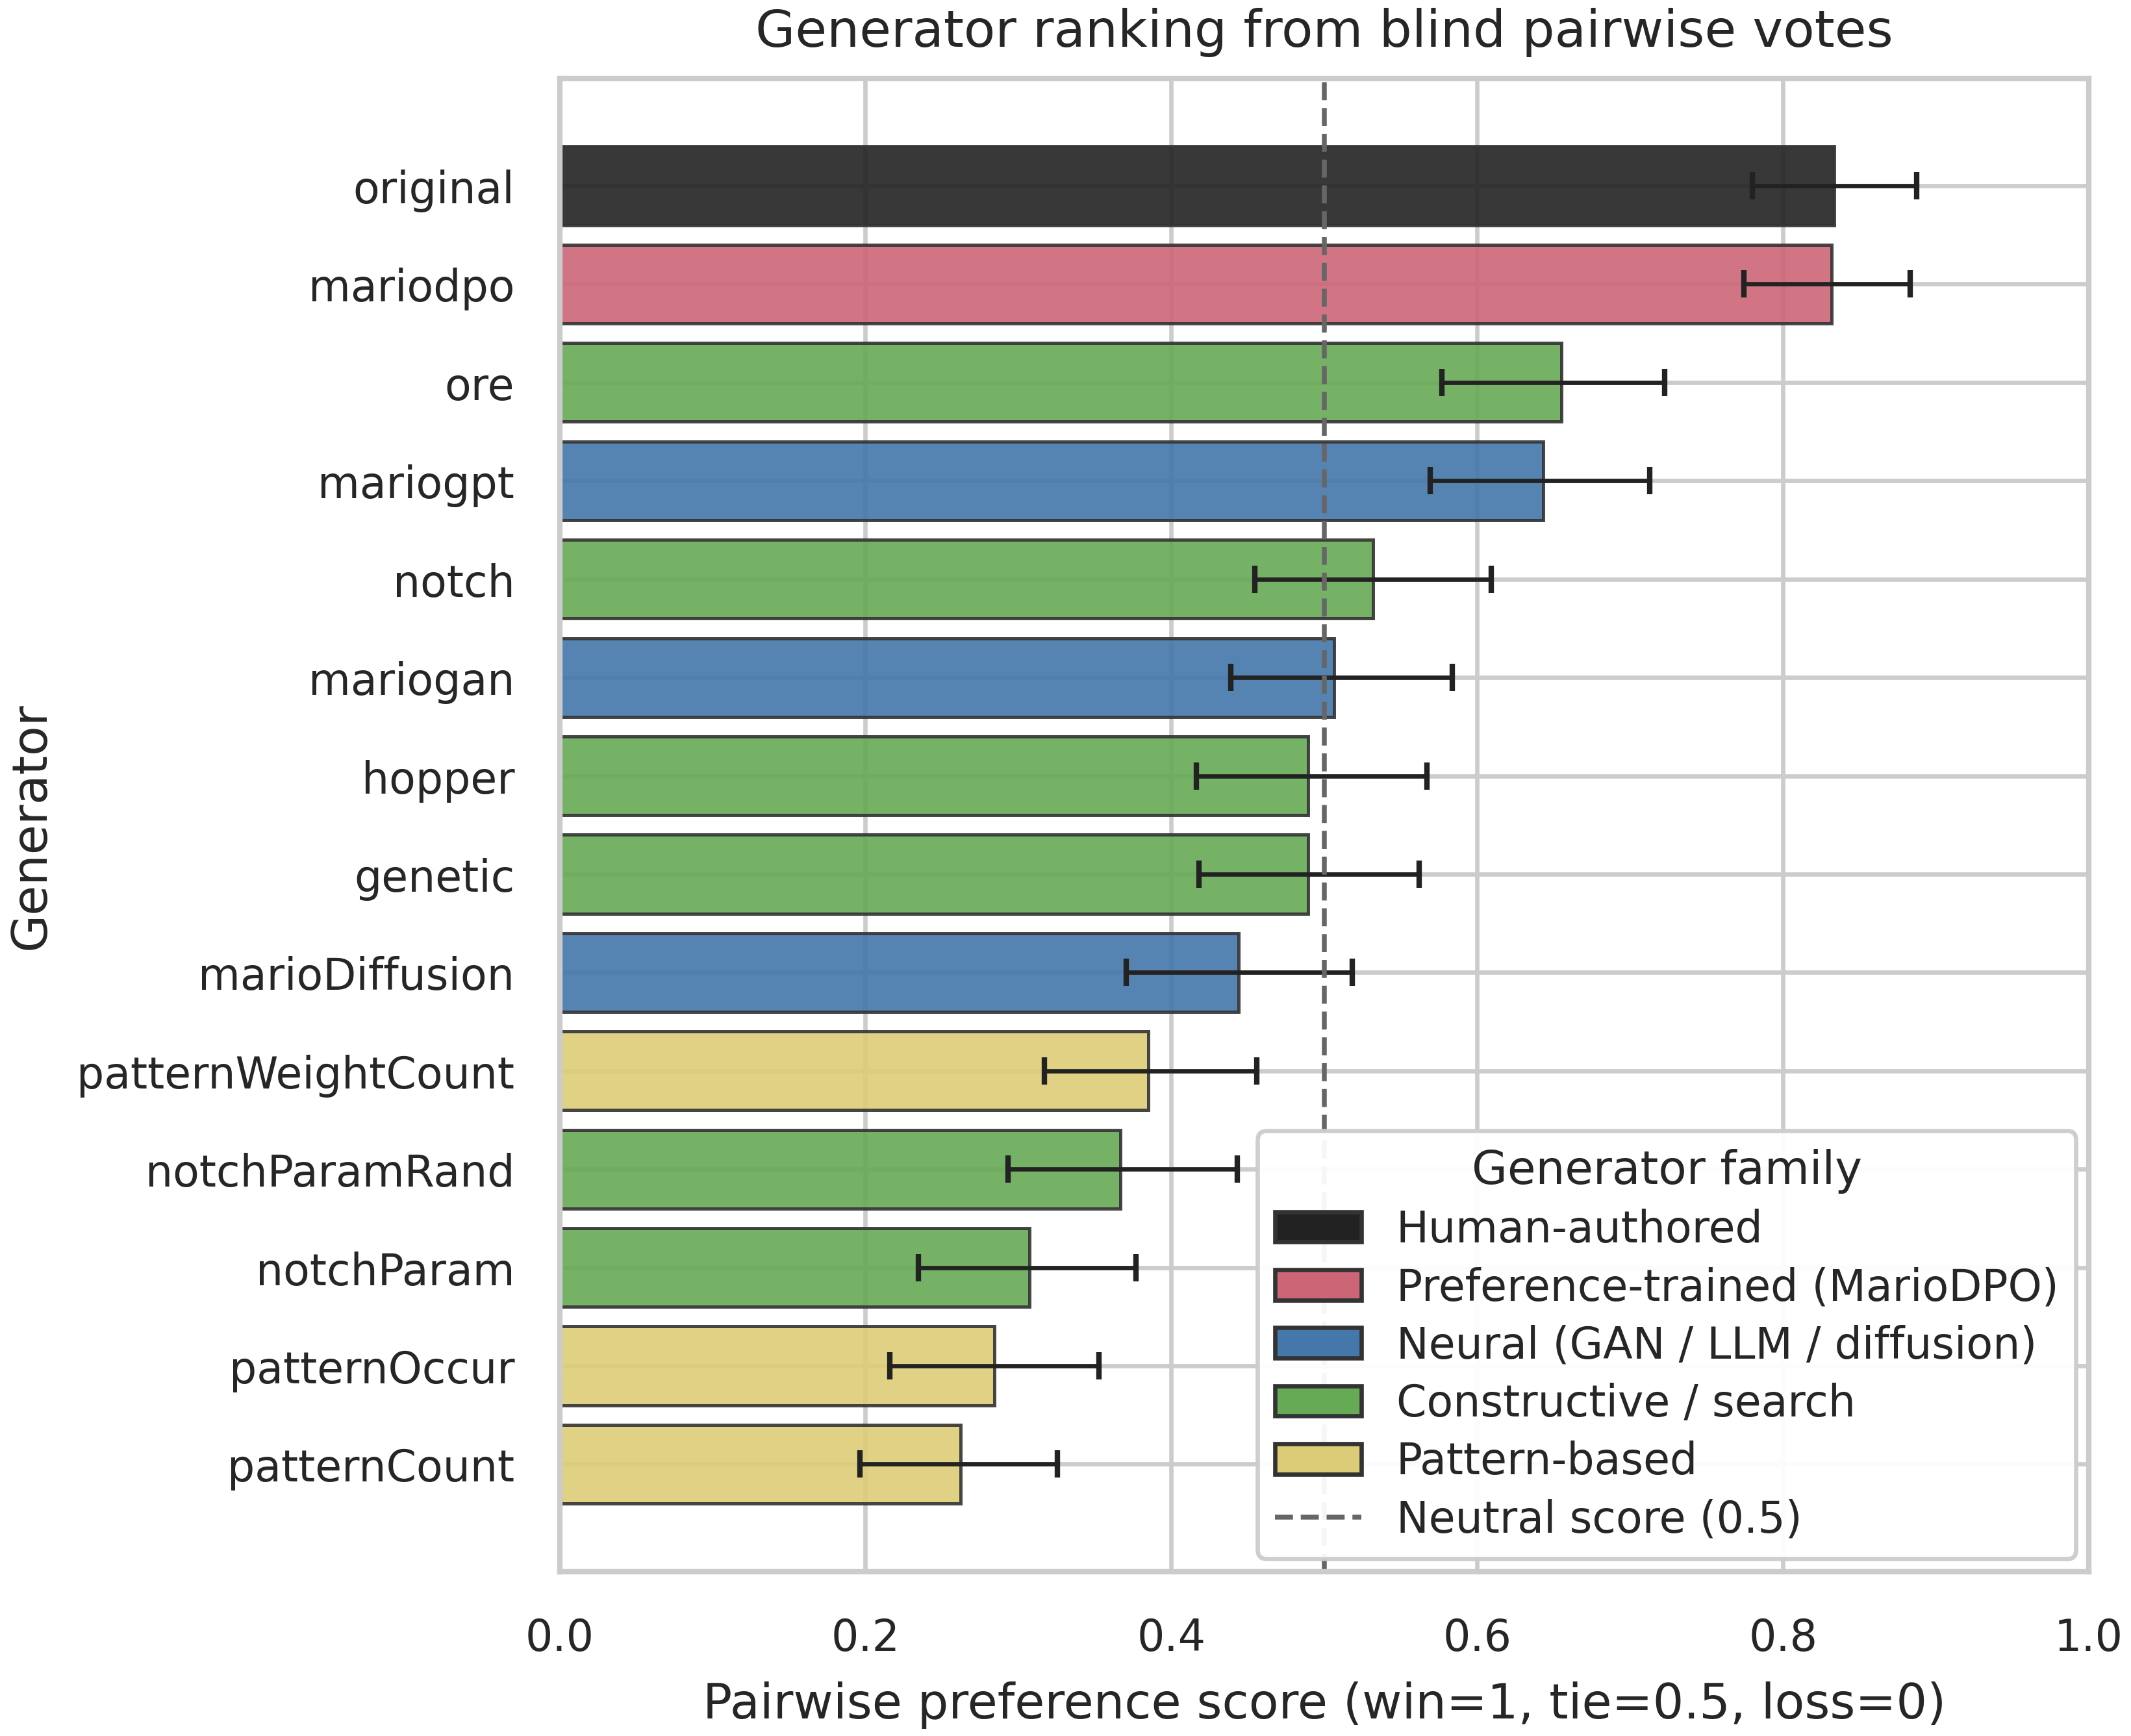
\includegraphics[width=0.95\textwidth]{eda_generator_ranking.png}
\caption{Generator ranking from blind pairwise votes. Bars show mean preference score, where win = 1, tie = 0.5, and loss = 0; horizontal intervals are 95\% bootstrap confidence intervals obtained by resampling votes. Bar colour encodes the generator family (human-authored, preference-trained, neural, constructive/search, and pattern-based), as shown in the in-plot legend.}
\label{fig:eda-generator-ranking}
\end{figure}

At the top of the ranking, the human-authored \texttt{original} baseline and \texttt{mariodpo} are nearly tied: \texttt{original} scores 0.833, while \texttt{mariodpo} scores 0.832. Both are well above the neutral 0.5 line. The next tier consists of \texttt{ore} (0.655) and \texttt{mariogpt} (0.643), followed by mid-table constructive and neural generators. The pattern-based generators occupy the bottom of the ranking: \texttt{patternWeightCount} scores 0.385, \texttt{patternOccur} scores 0.284, and \texttt{patternCount} scores 0.262.

As a first sanity check, the human-authored baseline remains at the top of the leaderboard, as expected if the votes reflect level quality. The export also includes MarioDPO, the preference-aligned generator developed in Chapter~\ref{ch:mariodpo}; we discuss its results in Section~\ref{sec:dpo-results}.

Figure~\ref{fig:eda-pairwise-confusion} gives the corresponding head-to-head matrix, with rows and columns ordered by the overall ranking. In this matrix, \texttt{original} and \texttt{mariodpo} achieve high win rates across most pairings, while the pattern-based generators lose consistently against nearly all opponents.

\begin{figure}[H]
\centering
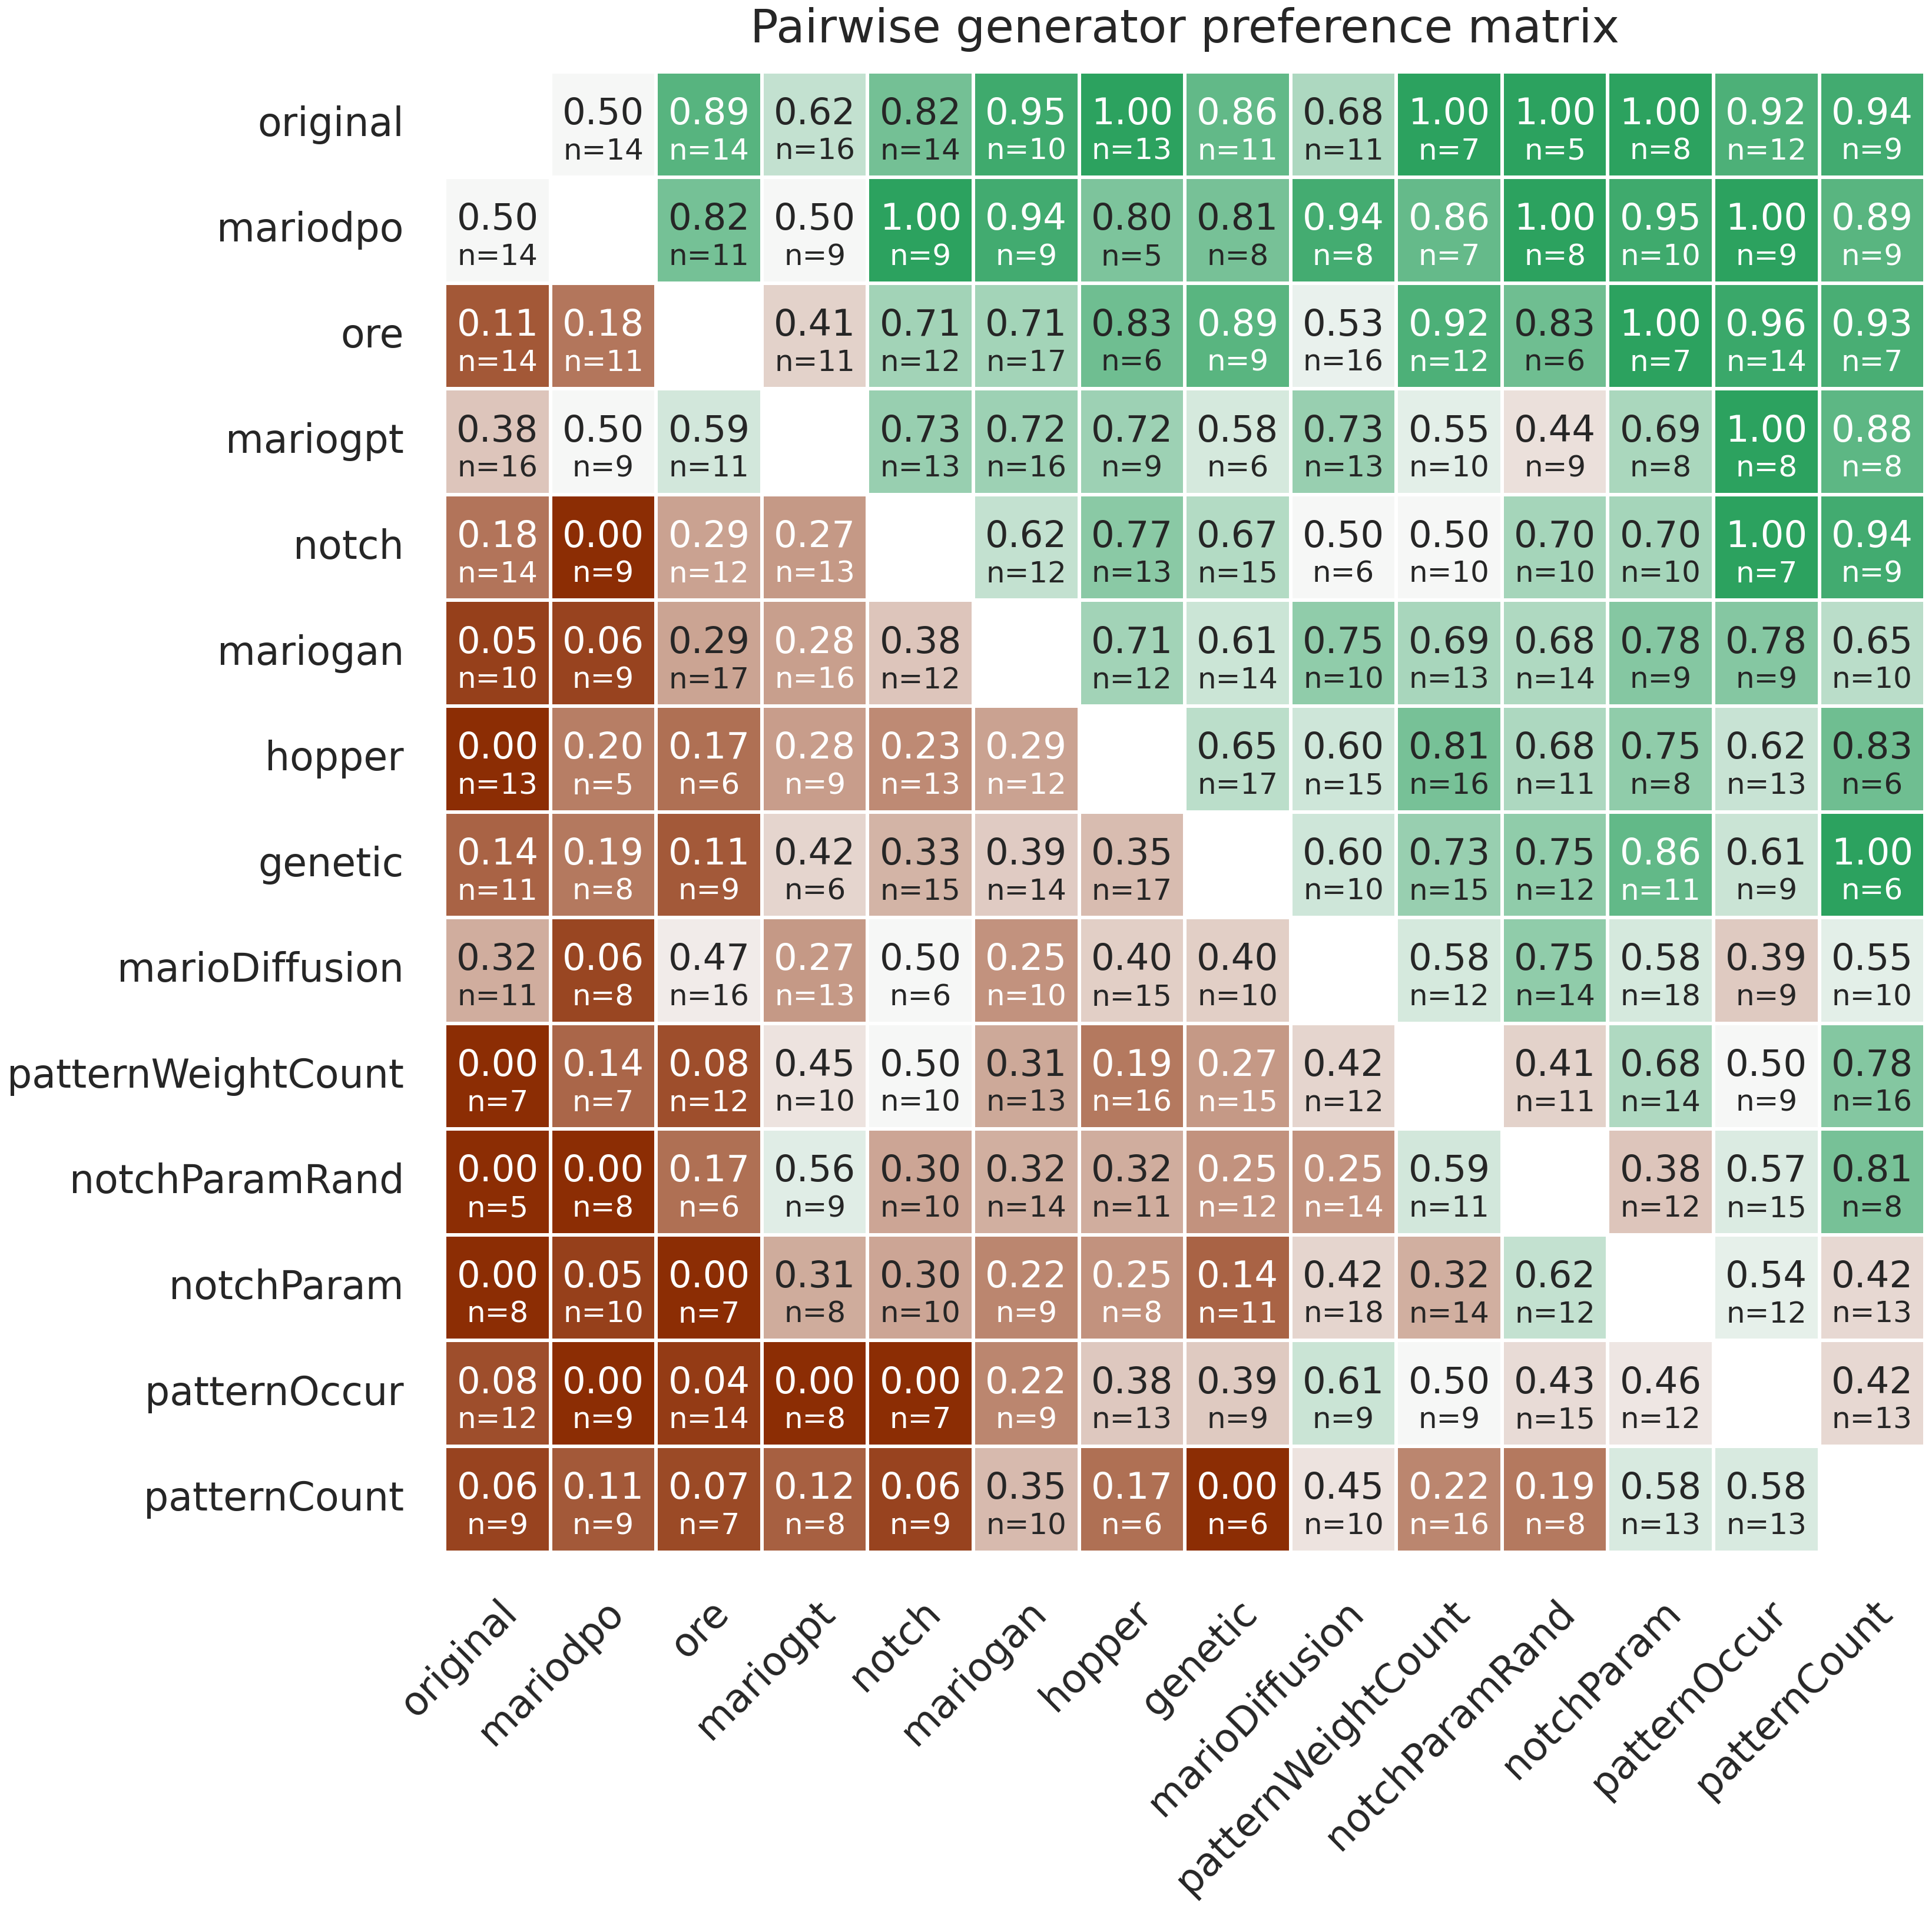
\includegraphics[width=0.95\textwidth]{eda_pairwise_confusion.png}
\caption{Pairwise generator preference matrix ordered by overall ranking. Each cell is the score rate for the row generator against the column generator, with ties counted as 0.5. Green indicates a higher score rate for the row generator.}
\label{fig:eda-pairwise-confusion}
\end{figure}

% ===================================================================
\section[Player Engagement and Preference Consistency]{Player Engagement and Preference Consistency}
\label{sec:eda-user-heterogeneity}

Aggregating individual votes into the single ranking of
Section~\ref{sec:eda-rankings} requires that the underlying player
population be reasonably consistent. This section examines how votes are
distributed across anonymous player IDs and whether their preferences align.
Figure~\ref{fig:eda-engagement} shows votes over time, votes per anonymous player ID, and cumulative vote contribution.

\begin{figure}[H]
\centering
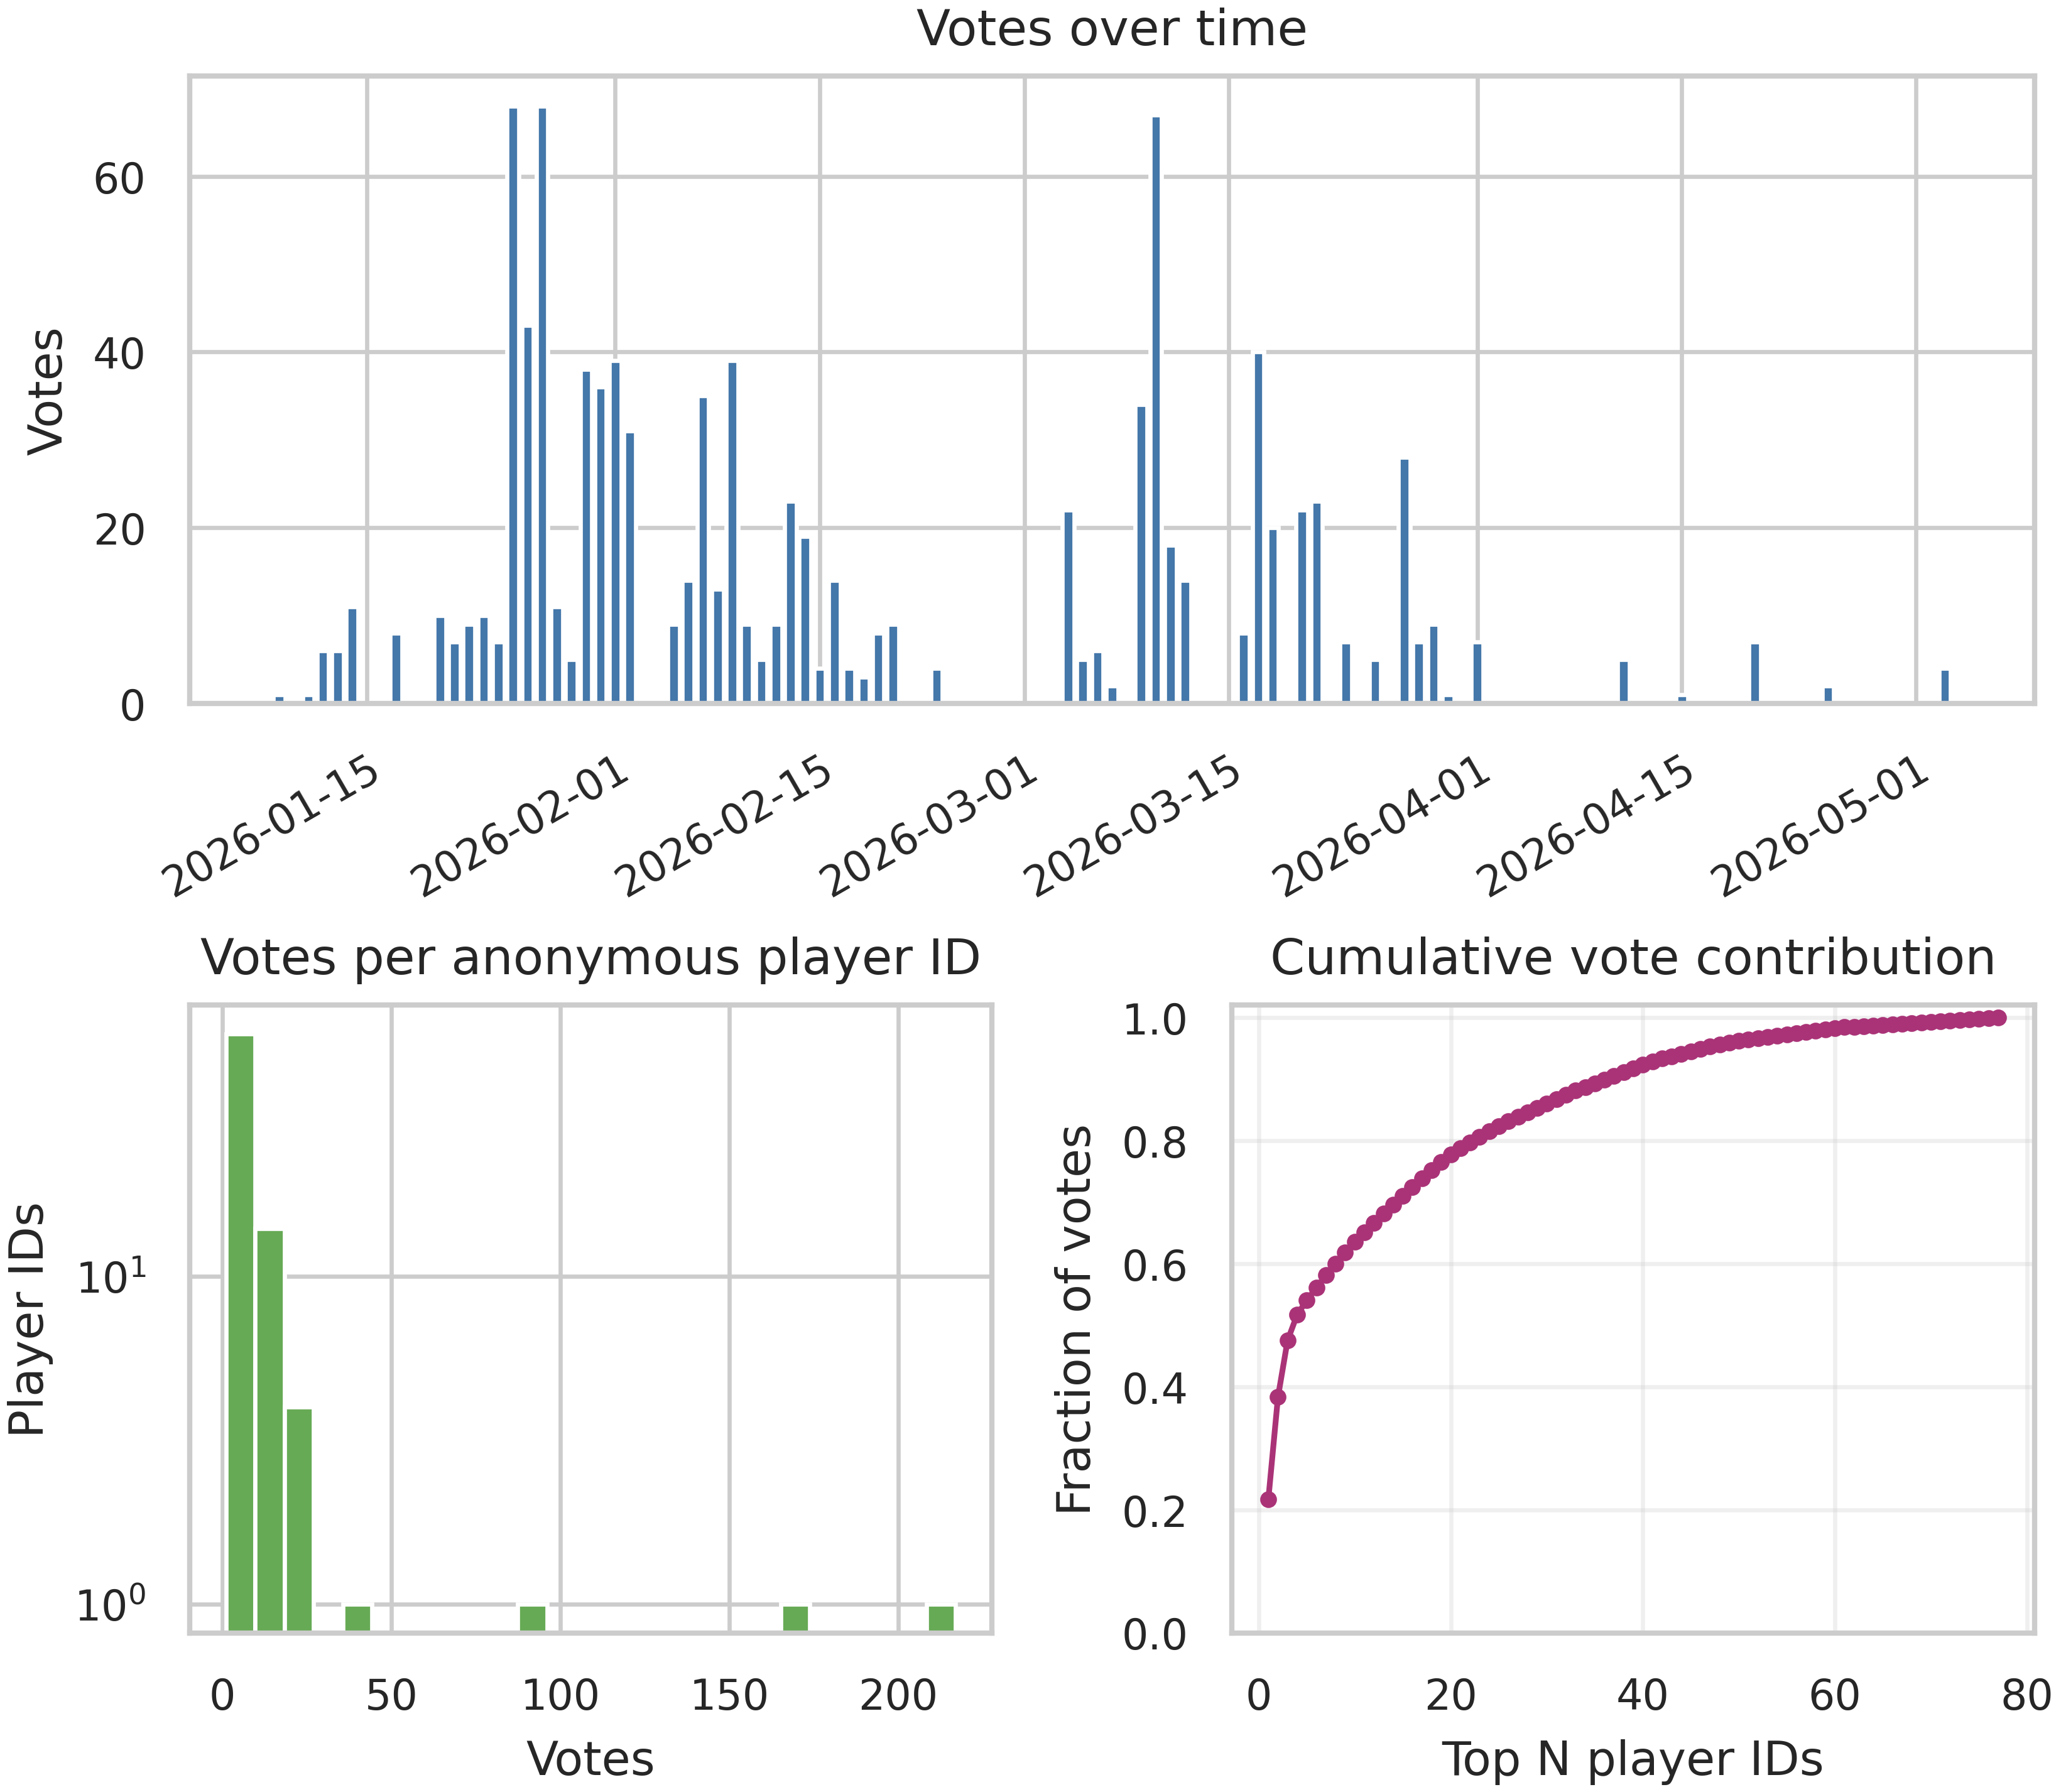
\includegraphics[width=\textwidth]{eda_engagement.png}
\caption{Engagement concentration across anonymous player IDs.}
\label{fig:eda-engagement}
\end{figure}

The vote distribution is heavily concentrated. Among the 77 anonymous player IDs in the vote table, the median player ID contributes 6 votes, while the most active ID contributes 217 votes. The top 5 IDs account for 54\% of the analyzed votes, and the top 10 account for 63.5\%. Consequently, aggregate generator scores reflect both broad participation and the preferences of a small number of highly active contributors.

Figure~\ref{fig:eda-user-heatmap} examines the player-by-generator preference matrix for anonymous player IDs with at least five votes. Each cell is the mean score assigned by a player ID when that generator appeared. Missing player-generator combinations are filled with the neutral value 0.5 only for visualization and clustering.

\begin{figure}[H]
\centering
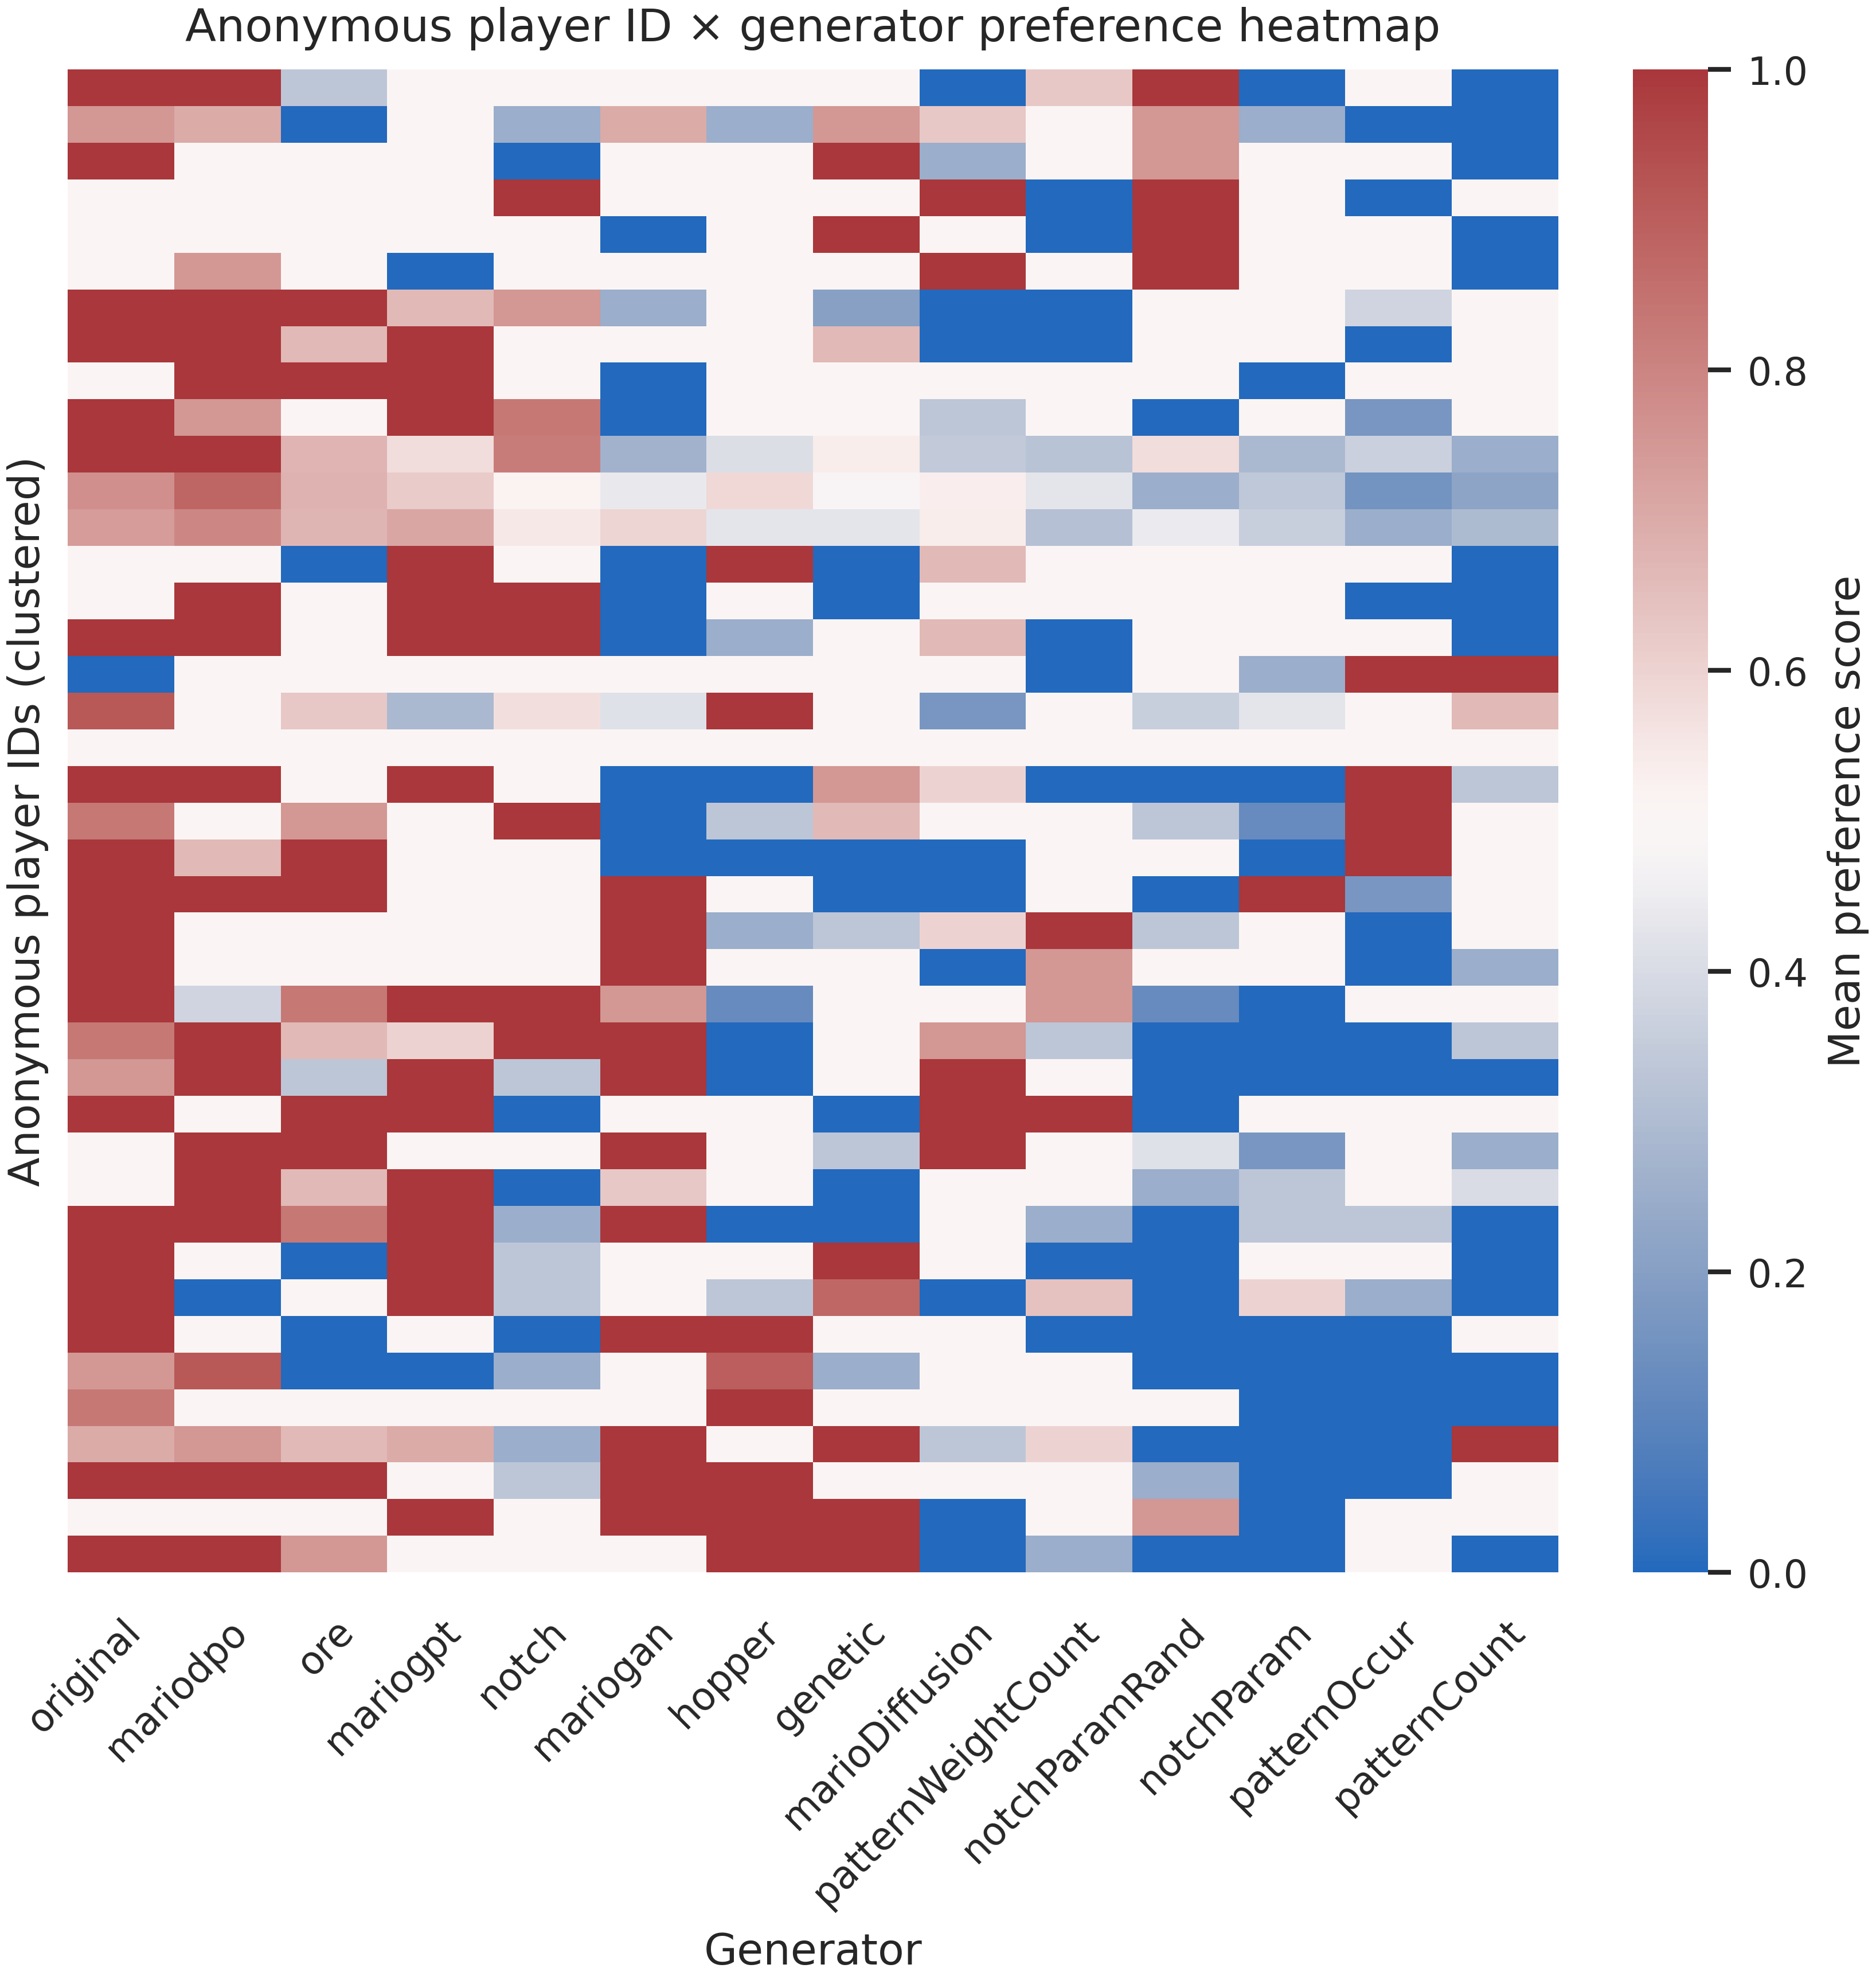
\includegraphics[width=\textwidth]{eda_user_generator_heatmap.png}
\caption{Preference heatmap of anonymous player IDs against generators.
Each row is a single anonymous player ID with at least five votes, and each
cell is that player's mean preference score for the generator in that column
(win = 1, tie = 0.5, loss = 0). Rows are ordered by hierarchical
clustering (Ward's method on Euclidean distances between players'
generator-score vectors) so that players with similar preference profiles are
placed next to one another. Columns follow the global generator ranking.}
\label{fig:eda-user-heatmap}
\end{figure}

Despite some individual variation, players largely agree on
which generators perform well and which perform poorly: most rows score the top-ranked
generators highly and the bottom-ranked generators low, with only mild
disagreement on the mid-table generators. Because the votes reflect a shared preference signal across players, they can be combined into a single
leaderboard (Section~\ref{sec:eda-rankings}) and used as a training signal
in Chapter~\ref{ch:mariodpo}.

% ===================================================================
\section{What Static Metrics Can and Cannot Tell Us}
\label{sec:eda-static-expressive-range}

This section examines what can be learned about a generator from
the levels themselves, without player telemetry. Each ASCII tilemap is summarised by a set of descriptive quantities: how flat or hilly its terrain is, how
many enemies it contains, how often gaps occur, how many rewards it offers,
and how similar its columns are to one another. Computing the same
quantities for every generator allows us to test whether any of these structural properties correlate with the player
preference scores from Section~\ref{sec:eda-rankings}.

We compute the metrics directly from the ASCII level files. Linearity is the
coefficient of determination ($R^2$) of a least-squares line fitted to the
playable surface profile; it measures how well a straight line explains the
surface, so a higher $R^2$ corresponds to flatter, more predictable terrain, while a lower value indicates a more irregular
profile. Density metrics count solid,
enemy, reward, and gap structure per tile or per level column. Leniency
combines gap density, enemy density, maximum gap width, rewards, and blocks
into a single descriptive score; because leniency definitions in
the PCG literature are not mutually comparable, we use this formulation only for within-study comparisons among the 14 generators. Diversity is estimated with tile/column entropy, the unique-column
ratio, the compression ratio, and gzip normalized compression distance (NCD).

Table~\ref{tab:eda-static-metrics} reports these metrics per
generator, ordered by preference score.

\begin{table}[H]
\centering
\footnotesize
\setlength{\tabcolsep}{3.5pt}
\begin{tabular}{@{} l r r r r r r r @{}}
\toprule
\textbf{Generator} & \textbf{Score} & \textbf{Levels} & \textbf{Linearity} & \textbf{Leniency} & \textbf{Gap dens.} & \textbf{Enemy dens.} & \textbf{NCD} \\
\midrule
original           & 0.83 & 15  & 0.02 & 0.61 & 0.18 & 0.08 & 0.83 \\
mariodpo~(ours)           & 0.83 & 200 & 0.06 & 0.67 & 0.14 & 0.09 & 0.81 \\
ore                & 0.65 & 100 & 0.11 & 0.63 & 0.16 & 0.06 & 0.85 \\
mariogpt           & 0.64 & 100 & 0.10 & 0.55 & 0.22 & 0.06 & 0.76 \\
notch              & 0.53 & 100 & 0.12 & 0.70 & 0.10 & 0.02 & 0.75 \\
mariogan           & 0.51 & 100 & 0.04 & 0.62 & 0.10 & 0.07 & 0.73 \\
hopper             & 0.49 & 100 & 0.17 & 0.63 & 0.11 & 0.12 & 0.73 \\
genetic            & 0.49 & 100 & 0.03 & 0.73 & 0.05 & 0.03 & 0.77 \\
marioDiffusion     & 0.44 & 100 & 0.05 & 0.44 & 0.28 & 0.02 & 0.78 \\
patternWeightCount & 0.38 & 100 & 0.07 & 0.72 & 0.08 & 0.13 & 0.87 \\
notchParamRand     & 0.37 & 100 & 0.14 & 0.74 & 0.07 & 0.02 & 0.73 \\
notchParam         & 0.31 & 100 & 0.05 & 0.71 & 0.07 & 0.02 & 0.70 \\
patternOccur       & 0.28 & 100 & 0.05 & 0.70 & 0.08 & 0.17 & 0.87 \\
patternCount       & 0.26 & 100 & 0.15 & 0.72 & 0.05 & 0.25 & 0.83 \\
\bottomrule
\end{tabular}
\caption{Static expressive metrics by generator (May 2026 export),
ordered by the preference score of Section~\ref{sec:eda-rankings}. Linearity
is the surface-fit $R^2$; NCD is the mean within-generator normalised
compression distance.}
\label{tab:eda-static-metrics}
\end{table}

As Table~\ref{tab:eda-static-metrics} shows, static structure acts only as a
coarse filter. The four highest-scoring generators have similar
static profiles (linearity between 0.02 and 0.11, leniency between 0.55 and 0.67,
gap density between 0.14 and 0.22, and enemy density between 0.06 and
0.09), yet their preference scores span 0.64 to 0.83; none of the static
columns explains why players prefer \texttt{original} and
\texttt{mariodpo} over \texttt{ore} and \texttt{mariogpt} by nearly 0.2.
No individual metric separates strong from weak generators across the table either: the highest
leniency belongs to \texttt{notchParamRand} (0.74, score 0.37), the highest
structural diversity by NCD to \texttt{patternWeightCount} and
\texttt{patternOccur} (0.87, scores 0.38 and 0.28), and the lowest-ranked
\texttt{patternCount} has above-average linearity. Extreme values do flag
degenerate designs: \texttt{patternCount}'s enemy density (0.25) is roughly
triple that of any top-tier generator, and \texttt{marioDiffusion}'s leniency
(0.44) is the lowest in the corpus, but such extremes only identify obvious
failures.

The answer to RQ2 is therefore negative: structural metrics cannot
replace human votes when ranking generators, consistent with the gap
between computational metrics and player experience reported by
\citet{marino2015empirical}. Figure~\ref{fig:eda-expressive-range} illustrates this in the linearity--leniency plane: each generator occupies a distinct region, so the metrics describe structural differences between generators, yet neither the position nor the spread of these regions tracks the preference ranking.

\begin{figure}[H]
\centering
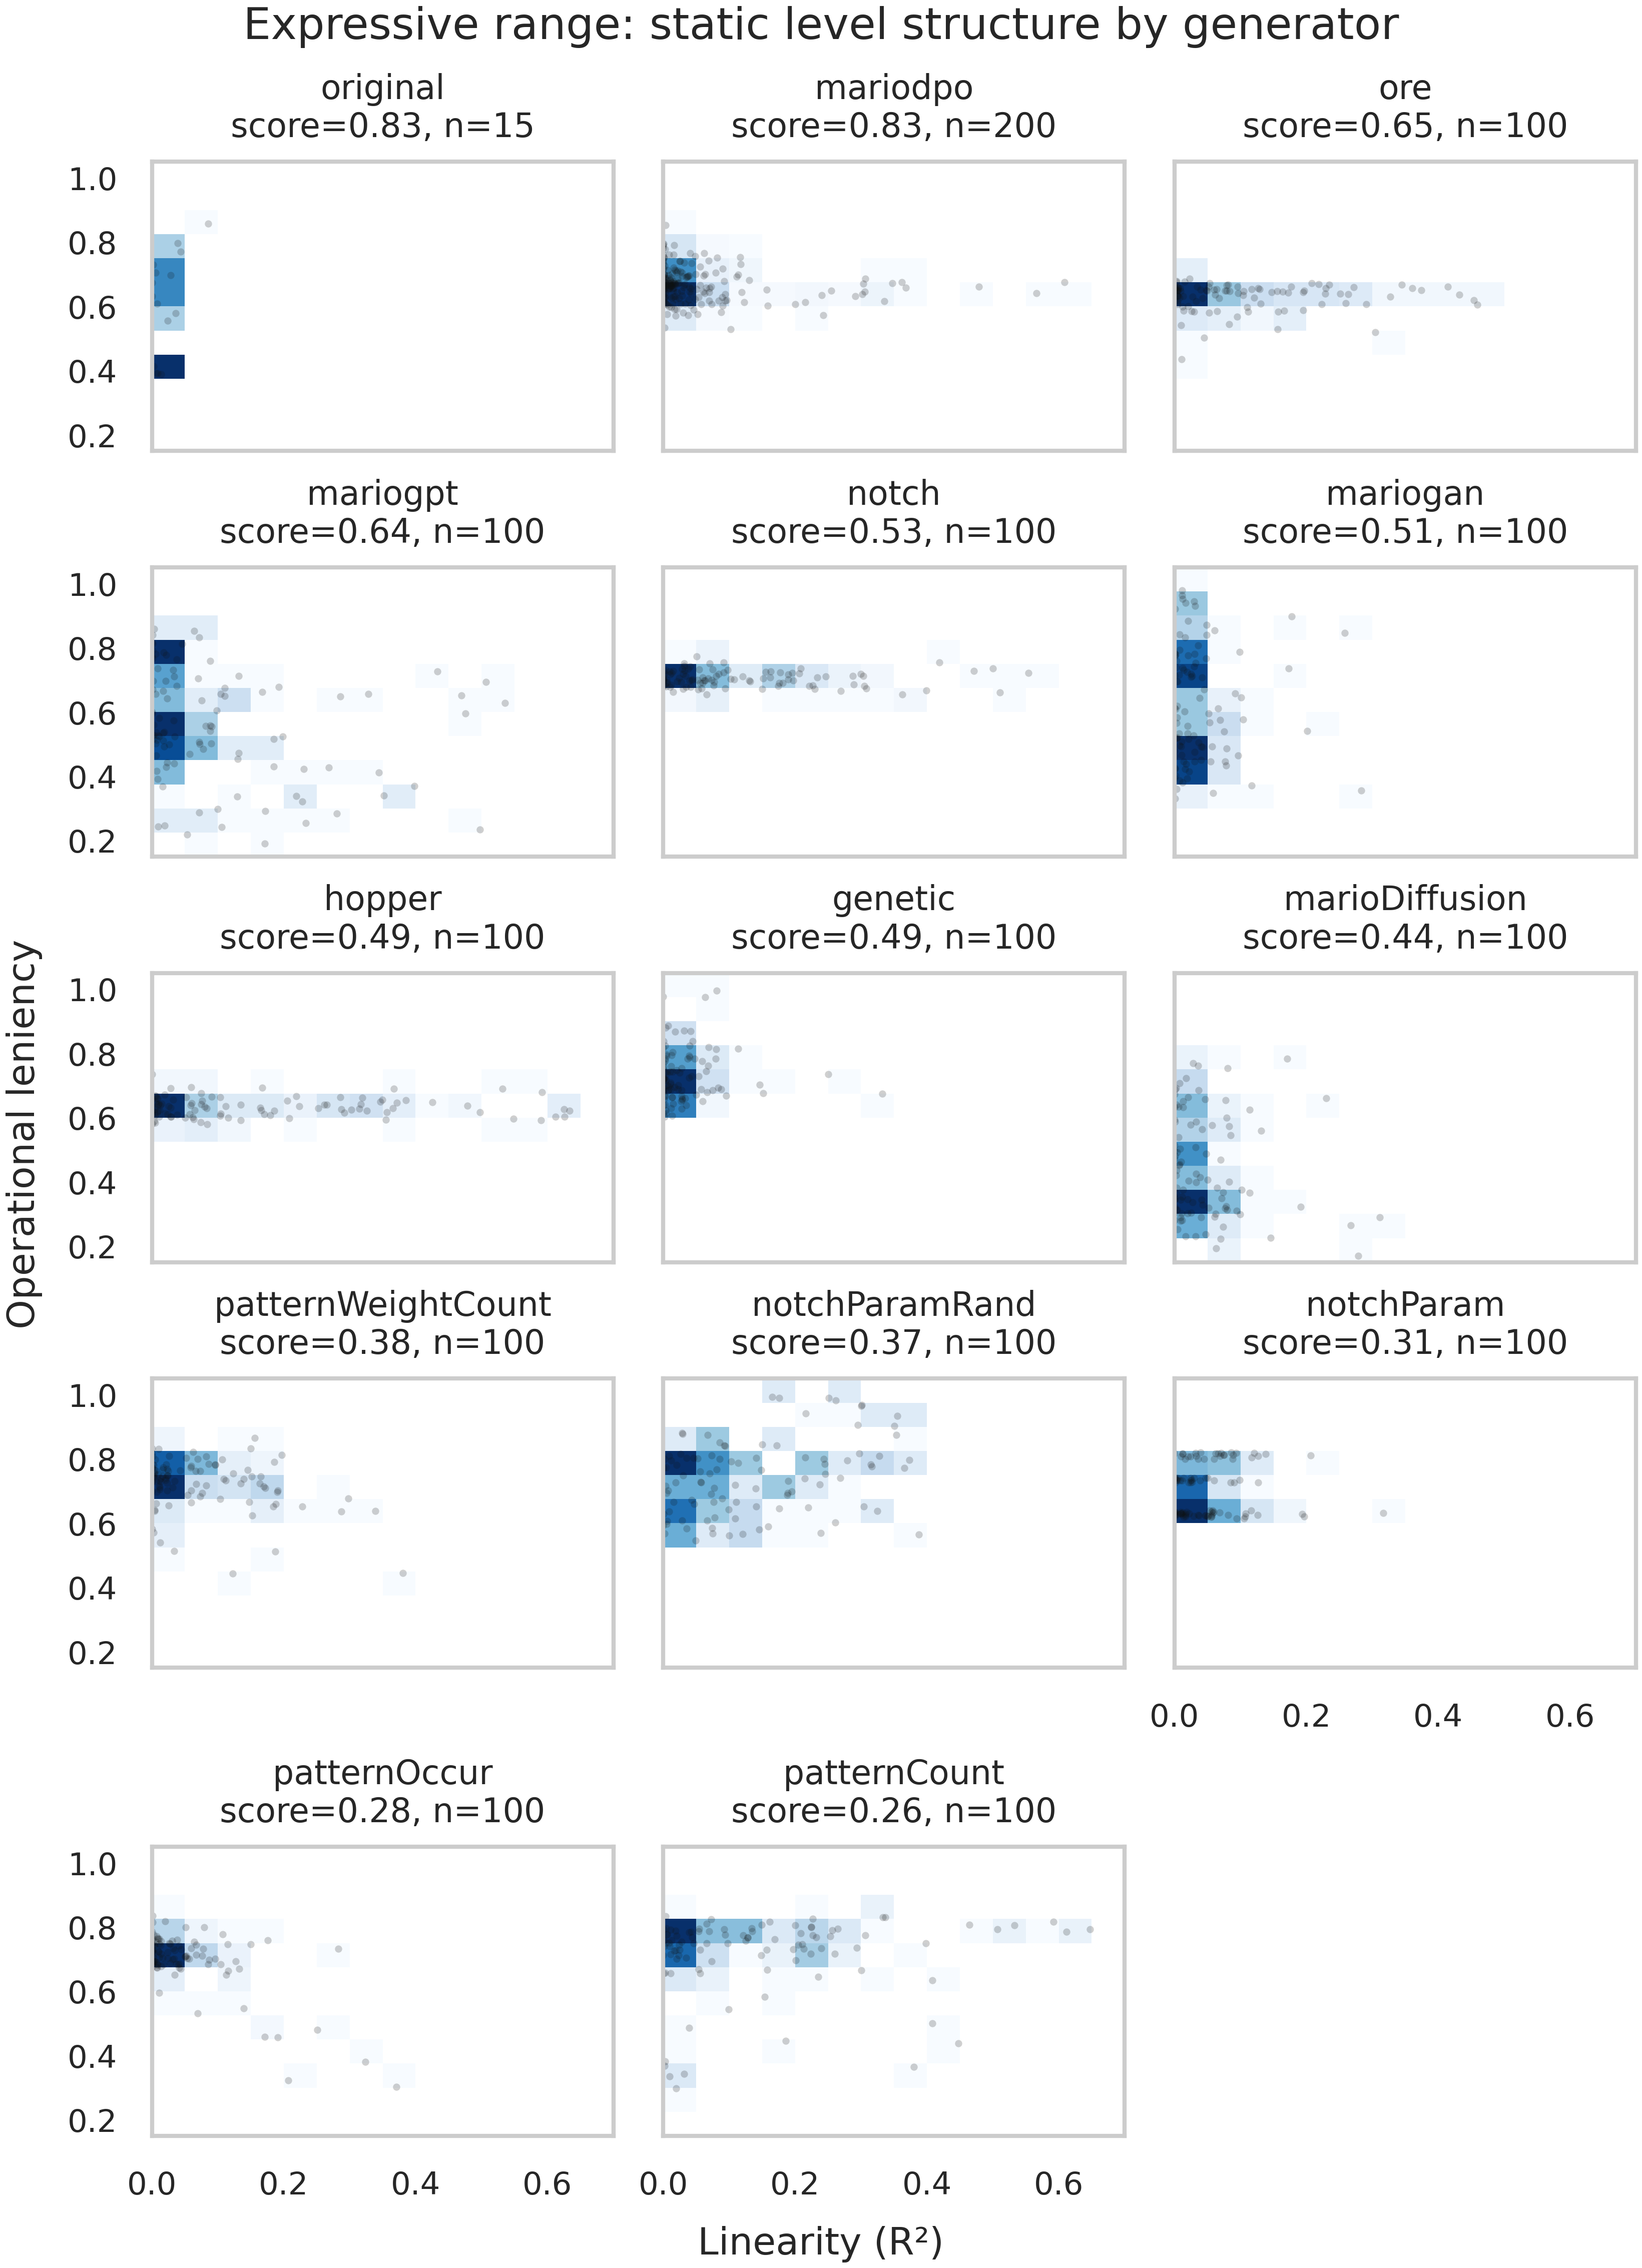
\includegraphics[width=\textwidth]{eda_expressive_range.png}
\caption{Expressive-range view of static level structure. Each subplot shows levels from one generator in the linearity--leniency plane, ordered by preference ranking.}
\label{fig:eda-expressive-range}
\end{figure}

% ===================================================================
\section{Why Levels Lose: Trajectories and Tags}
\label{sec:eda-trajectory-fingerprints}
\label{sec:eda-tag-semantics}

Although static structure does not explain the ranking, the battle records include
two additional data sources that help explain why levels \emph{lose}: where players fail
(gameplay trajectories) and how they label the levels (tags).

For each generator, Figure~\ref{fig:eda-trajectory-stacks} overlays all recorded Mario paths as thin red traces, showing where players actually moved during their single attempt per level.

\begin{figure}[H]
\centering
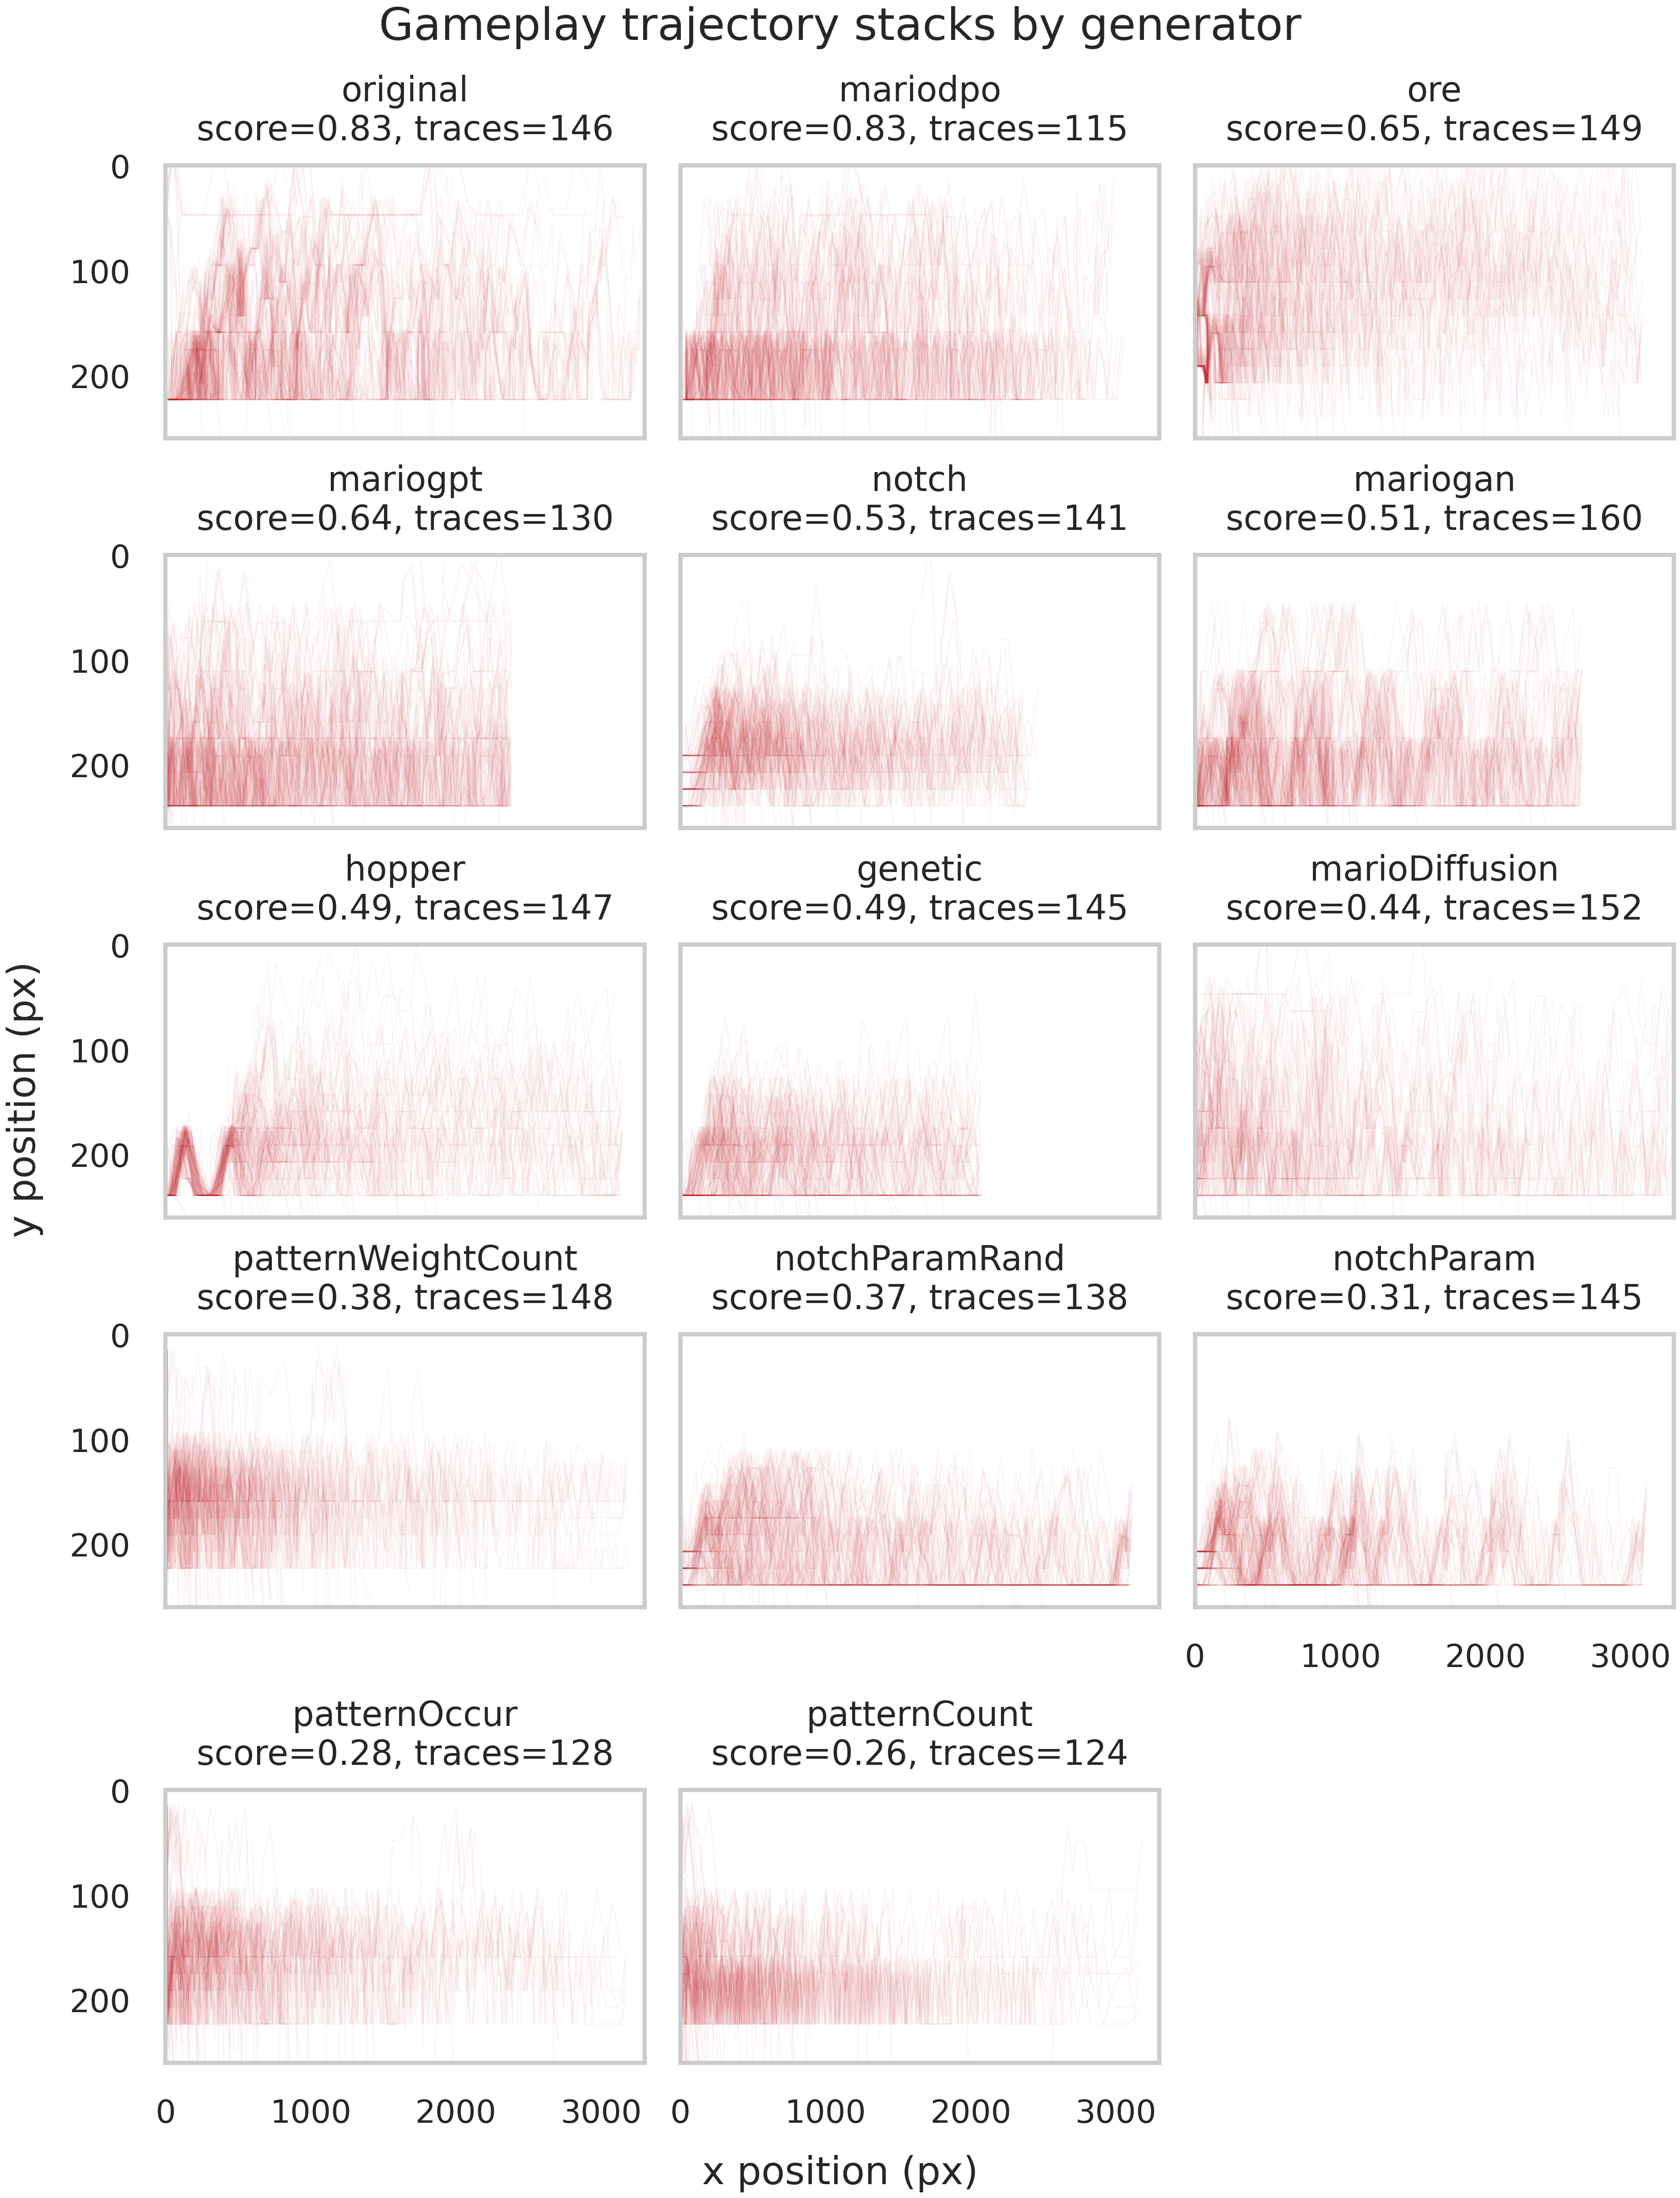
\includegraphics[width=\textwidth]{eda_trajectory_stacks.png}
\caption{Stacked gameplay trajectories by generator. Each subplot overlays all recorded trajectories for one generator as thin red traces on a white background, ordered by preference score. The vertical axis is inverted to match screen coordinates.}
\label{fig:eda-trajectory-stacks}
\end{figure}

The trajectory plots show clear differences in player progress. For the top generators, traces
extend far into the level and span a wide vertical band: the median maximum
progress is 1126.5 pixels for \texttt{original} and 988.0 pixels for
\texttt{mariodpo}. For the lowest-ranked generators, traces cluster near the start and terminate
early: \texttt{patternCount} has a median maximum progress of only 174.5
pixels, and 63\% of its recorded deaths fall into a single early horizontal
bin. In these levels, players encounter an immediate obstacle within the first screens.

Player-assigned tags add a qualitative diagnostic layer to the binary votes.
Figure~\ref{fig:eda-tag-semantics} summarizes tag frequency, tag rate by generator, tag co-occurrence, and outcome distribution when each tag is present. The most common tags are \texttt{impossible} (87 assignments), \texttt{fun} (56), \texttt{too\_hard} (55), \texttt{boring} (49), \texttt{creative} (39), \texttt{broken\_graphics} (22), and \texttt{too\_easy} (21).

\begin{figure}[H]
\centering
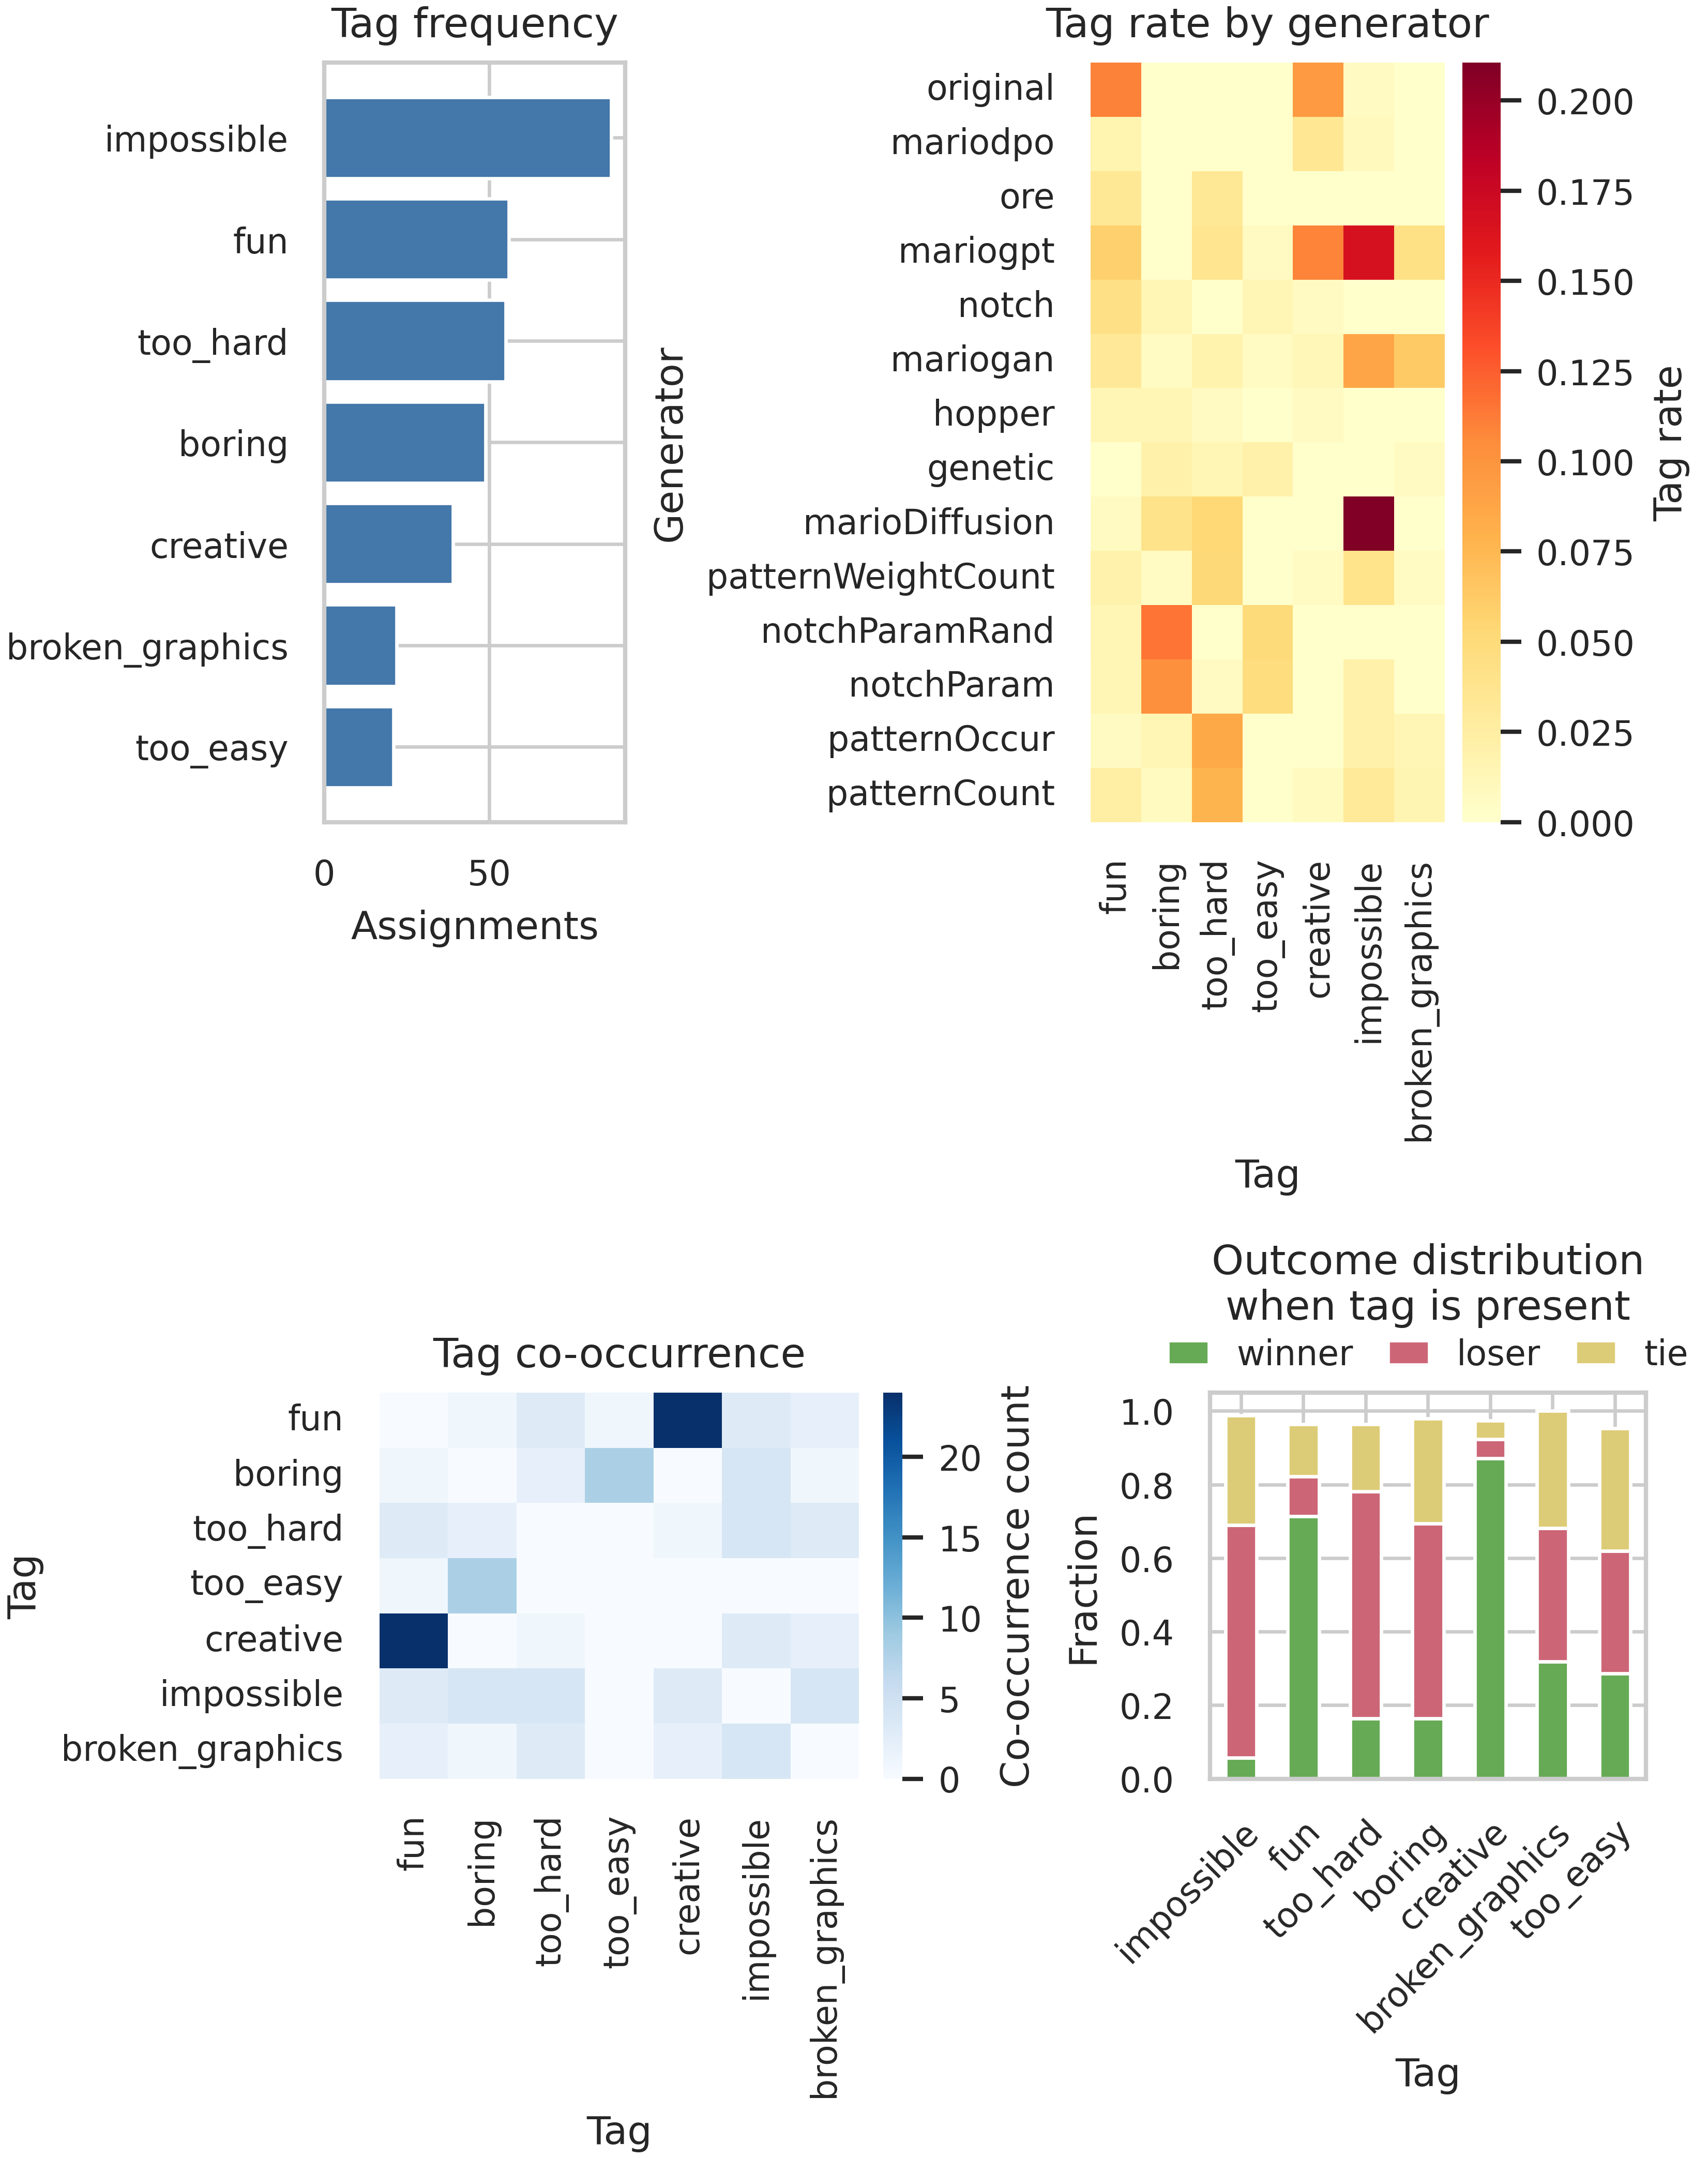
\includegraphics[width=\textwidth]{eda_tag_semantics.png}
\caption{Tag semantics summary. The panels show tag frequency, tag rate by generator, tag co-occurrence, and the outcome distribution for tagged sides.}
\label{fig:eda-tag-semantics}
\end{figure}

Positive tags correspond closely with winning outcomes: sides tagged \texttt{creative} win 87\% of the time and sides tagged \texttt{fun} win 71\% of the time. Negative tags behave differently, \texttt{impossible}, \texttt{too\_hard}, and \texttt{boring} are much more common on losing sides. The tag-by-generator heatmap also separates generator failure modes, distinguishing generators marked as impossible or too hard from those rejected as boring or visually broken.

Together, trajectories and tags point to the same mechanism: the main diagnosable cause of lost battles is early frustration. Levels that kill the
player repeatedly near the start are the same levels tagged
\texttt{impossible} and \texttt{too\_hard}, and they consistently lose. While \texttt{fun} and \texttt{creative} co-occur with winning levels,
Section~\ref{sec:eda-static-expressive-range} showed no simple structural formula for positive enjoyment. This asymmetry motivates the design of the judge function in the next
section.

% ===================================================================
\section{The Judge Function}
\label{sec:dpo-judge}

Chapter~\ref{ch:mariodpo} trains a generator on preference pairs, and
the 473 usable human votes in the January training snapshot
(Table~\ref{tab:eda-timeline}) are too few on their own to fine-tune a sequence model.
We therefore need an automatic way to label additional level pairs. Because no
combination of static metrics reproduces the human ranking
(Section~\ref{sec:eda-static-expressive-range}), we do not attempt to model
enjoyment directly; instead, we target the failure modes identified in
Section~\ref{sec:eda-tag-semantics}. The judge function $J_{final}$ is
designed as a coarse filter that separates flawed levels
from plausible ones.

The judge is a weighted sum of five interpretable terms:
%
\begin{equation}
\label{eq:dpo-j-final}
\begin{aligned}
J_{final} ={} & w_{style}\frac{1}{1 + D_M}
- w_{gap}\,\mathit{GapPenalty}
+ w_{comp}\,\mathit{Completion} \\
& + w_{vert}\,\frac{\sigma_y}{50}
+ w_{flow}\,(1 - \mathit{Hesitation}),
\end{aligned}
\end{equation}
%
where $D_M$ is the Mahalanobis distance from a level's feature vector
to the centroid of the original Nintendo levels, rewarding proximity to the
human-authored region of feature space; $\mathit{GapPenalty}$ penalises
fragmented, pit-heavy ground; $\mathit{Completion}$ is the fraction of the
level traversed; $\sigma_y$ is the standard deviation of Mario's vertical
position along a trajectory; and $\mathit{Hesitation}$ is the fraction of
trajectory time spent at near-zero horizontal velocity.

Because the last three quantities depend on gameplay trajectories and the judge must score
newly generated levels that no human has played, they are computed by
running an A* agent through each candidate level. Using an agent as
a stand-in for a player is standard practice in PCG evaluation
(Section~\ref{subsec:bg-eval-agents}), though the agent's superhuman play policy reinforces the role of $J_{final}$ as a coarse filter.

The weights (Table~\ref{tab:dpo-judge-weights}) were selected by a
grid search maximising pairwise agreement with the human votes under
fixed term signs. The
gap penalty receives the largest weight, consistent with early frustration being the clearest
failure mode in the arena data
(Section~\ref{sec:eda-tag-semantics}), while the remaining terms
incorporate the structural and trajectory features from
Sections~\ref{sec:eda-static-expressive-range}
and~\ref{sec:eda-trajectory-fingerprints}.

\begin{table}[H]
\centering
\begin{tabular}{@{} l c p{7.2cm} @{}}
\toprule
\textbf{Term} & \textbf{Weight} & \textbf{Role} \\
\midrule
$w_{gap}$   & 0.50 & penalise the dominant failure mode: fragmented, pit-heavy structure \\
$w_{style}$ & 0.32 & reward proximity to the original-level centroid \\
$w_{vert}$  & 0.26 & reward vertical variety \\
$w_{comp}$  & 0.20 & reward completion of the level \\
$w_{flow}$  & 0.10 & penalise hesitation and poor flow \\
\bottomrule
\end{tabular}
\caption{Judge-function weights, obtained by grid search over
interpretable weights maximising pairwise agreement with human votes.}
\label{tab:dpo-judge-weights}
\end{table}

Aggregated by generator on the January snapshot, $J_{final}$
correlates with human win rate at $r_s = 0.736$ ($p = 0.0027$). Because the weights were fitted on the same snapshot, this correlation represents an in-sample check across the 14
generators: it confirms that
the judge reproduces the broad quality tiers by placing
degenerate, frustrating generators below plausible ones.

This level of discrimination is sufficient for how Chapter~\ref{ch:mariodpo}
uses $J_{final}$: the judge only labels pairs of levels with a clear score margin so that training includes diverse examples
of flawed structure to avoid, while the strongly upweighted human votes provide the positive preference signal. The practical test of this setup is whether the resulting generator wins blind
human votes after deployment.

% ===================================================================
\section[Summary: A Reliable but Sparse Signal]{Summary: A Reliable but Sparse Signal}
\label{sec:eda-summary}

The chapter yields five main findings:
\begin{enumerate}[nosep]
    \item \textbf{Measurement works}: blind pairwise votes produce a stable ranking, with \texttt{original} and \texttt{mariodpo} nearly tied at the top ($\approx$0.83) and pattern-based generators at the bottom.
    \item \textbf{Players agree}: the same generators score high or low across the anonymous population, so the aggregate ranking reflects shared preference.
    \item \textbf{Static metrics cannot rank}: the top generators have near-identical static profiles and no metric column separates strong from weak; structure acts only as a coarse filter for degenerate designs.
    \item \textbf{Failure is diagnosable}: early, concentrated deaths and \texttt{impossible}/\texttt{too\_hard} tags mark losing levels, while \texttt{fun} and \texttt{creative} align with wins but show no structural recipe.
    \item \textbf{A coarse judge suffices for labelling}: combining the failure signals yields $J_{final}$, which reproduces the quality tiering in-sample ($r_s = 0.736$) by catching easy-to-spot failures.
\end{enumerate}

Two properties of the vote signal matter for what follows. It is
reliable: anonymous players largely agree on which generators are good
(Section~\ref{sec:eda-user-heterogeneity}). It is also sparse: the
January training snapshot contains only 473 usable non-tie votes
(Table~\ref{tab:eda-timeline}), far too few to fine-tune a sequence model
directly. The next chapter therefore trains on the human votes as the primary
preference signal and uses the judge only to broaden negative
coverage---closing the loop from measurement to generation.


\chapter{MarioDPO --- Preference-Aligned Level Generation}
\label{ch:mariodpo}


\section[Motivation: From Sparse Votes to a Training Signal]{Motivation: From Sparse Votes to a Training Signal}
\label{sec:dpo-motivation}

The previous chapter established three results. First, blind pairwise
votes produce a reliable ranking signal, as anonymous players largely agree on
which generators perform well (Section~\ref{sec:eda-user-heterogeneity}). Second,
no automated metric substitutes for that signal (Section~\ref{sec:eda-static-expressive-range}), which motivates training
MarioDPO directly on player preferences. Third, frustrating and uncompletable structure is reliably
identifiable, and the judge function of Section~\ref{sec:dpo-judge} can label it
cheaply and at scale. However, the January 2026 training snapshot contains only 473 usable non-tie
votes, which is orders of magnitude smaller than the preference datasets used to align
language models (e.g., the 64K comparisons of \citet{stiennon2020learning})
and too small to fine-tune a level generator on human votes alone.

MarioDPO therefore combines three ingredients. The base model is the
published MarioGPT checkpoint, so the generator already produces valid Mario
structure before preference optimisation begins. The 473 human
pairs, upweighted $10\times$, anchor training to human
judgements and carry the positive preference signal. Finally, the judge
function labels 2,606 additional synthetic pairs to steer the model away from common failure modes without
diluting the human preference objective.

MarioDPO consists of four components:
\begin{enumerate}[nosep]
  \item A column-major level representation that preserves the vertical structure
        of Mario tilemaps while remaining compatible with autoregressive
        sequence modelling;
  \item A base generator reusing the MarioGPT checkpoint;
  \item A preference dataset combining the human PCG Arena votes with
        synthetic pairs labelled by the judge function developed in
        Section~\ref{sec:dpo-judge}; and
  \item A DPO fine-tuning stage that aligns the base generator with
        the resulting preference signal.
\end{enumerate}

The design separates \emph{validity} from \emph{preference}.
Validity is enforced through representation choices, start/end constraints, and
deterministic post-processing
(Section~\ref{subsec:dpo-training-details}), whereas preference
is learned from human votes and the judge function. Because a level can be playable yet unengaging, MarioDPO trains the model to generate levels that
players prefer in blind A/B tests while handling structural validity separately.

Figure~\ref{fig:dpo-pipeline} summarises the composition of the training data.
The MarioGPT checkpoint provides the structural prior, PCG Arena provides
human comparisons, the judge function expands these comparisons into
a larger preference dataset, and DPO aligns the generator with the resulting
preference signal.

\begin{figure}[H]
\centering
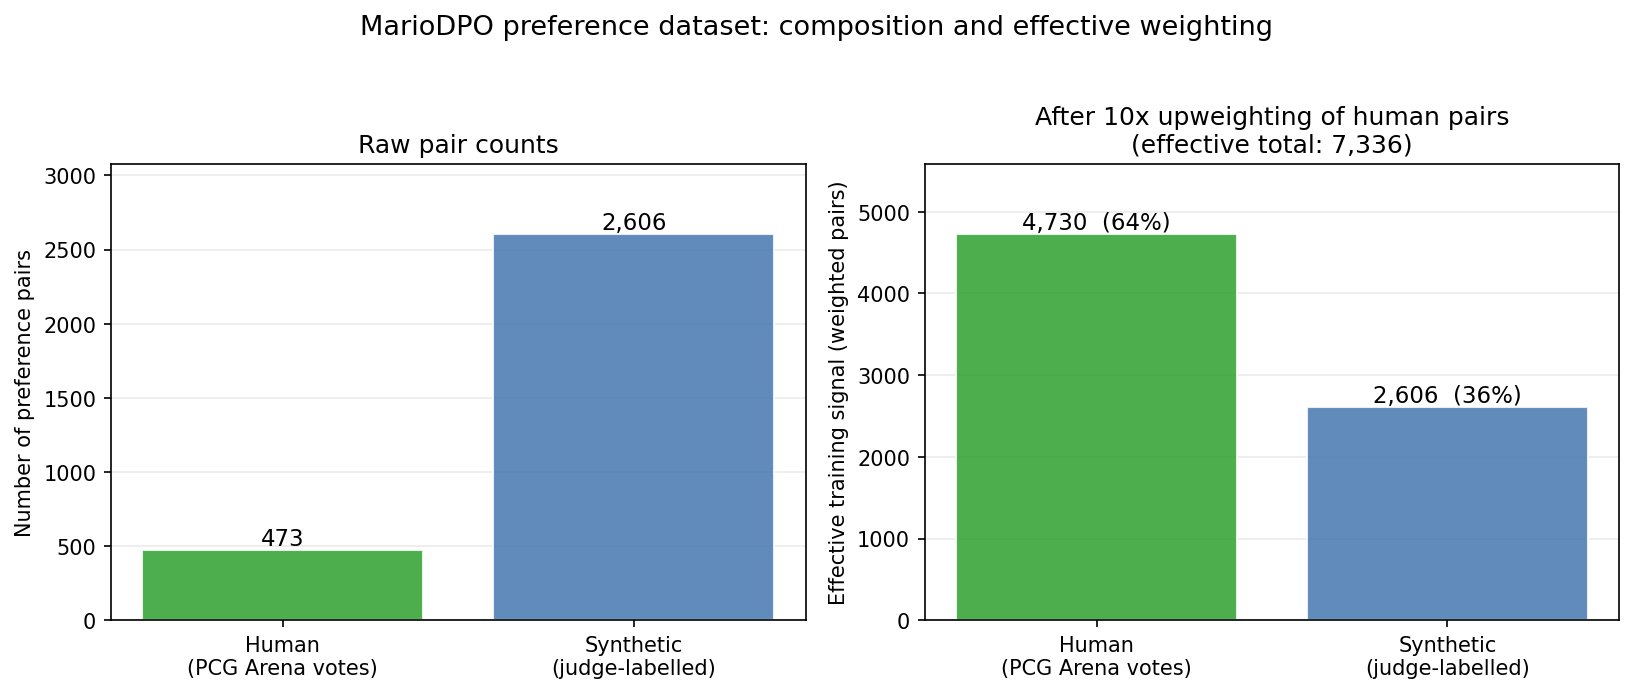
\includegraphics[width=0.9\textwidth]{dpo_training_data.png}
\caption{MarioDPO preference dataset: raw pair counts (left) and the same counts
after applying the $10\times$ upweighting of human PCG Arena pairs (right). The
few hundred human comparisons contribute roughly two thirds of the effective
training signal, while pairs labelled by the judge function
(Section~\ref{sec:dpo-judge}) primarily broaden coverage.}
\label{fig:dpo-pipeline}
\end{figure}

\section[Level Representation and Base Model]{Level Representation and Base Model}
\label{sec:dpo-tokenisation}

\subsection{Column-Major Tokenisation}
\label{subsec:dpo-representation}

Mario levels in this thesis are represented as ASCII tilemaps: each level is a
matrix of characters, with rows corresponding to vertical tile positions and
columns corresponding to horizontal progress through the level. The standard
height is 16 tiles; widths vary between generators, with the corpus average equal
to 193.8 tiles. The vocabulary contains 37 distinct tile characters,
dominated by empty space (\texttt{-}), solid blocks (\texttt{X}),
pipes (\texttt{|}, \texttt{<}, \texttt{>}, \texttt{[}, \texttt{]}), platforms
(\texttt{\%}), question blocks (\texttt{?}, \texttt{Q}), coins (\texttt{o}),
and enemies such as Goombas (\texttt{g}) and Koopas (\texttt{k}).

A naive row-major serialisation would place horizontally adjacent tiles next to
one another in the sequence, but would separate vertically adjacent tiles by an
entire row length. This is undesirable for Mario levels, where local vertical
relationships are essential: enemies stand on platforms, pipes occupy multiple
rows, and jumpable structures depend on the configuration of several tiles in a
column. MarioDPO therefore uses a column-major representation. Conceptually, the
level is decomposed into a sequence of 16-character columns,
%
\begin{equation}
\label{eq:dpo-columns}
c_t = (x_{1,t}, x_{2,t}, \ldots, x_{16,t}),
\end{equation}
%
where $x_{r,t}$ is the tile at row $r$ and column $t$. The autoregressive model
then predicts the next column in a flattened column-major
sequence. This preserves vertical locality while still allowing standard
left-to-right generation.

Table~\ref{tab:dpo-representation} summarises the representation choices.
Post-processing acts on the same column units when enforcing ground
continuity, start safety, and flag placement.

\begin{table}[H]
\centering
\caption{MarioDPO level representation and tokenisation choices.}
\label{tab:dpo-representation}
\begin{tabular}{ll}
\toprule
\textbf{Property} & \textbf{Choice} \\
\midrule
Level format & ASCII tilemap \\
Height & 16 rows \\
Average width in corpus & 193.8 tiles \\
Vocabulary size & 37 tile characters \\
Sequence order & Column-major, left to right \\
Validity constraints & Safe start, bounded gaps, end flag, post-processing \\
\bottomrule
\end{tabular}
\end{table}

Training examples are obtained by sliding a window over the
column-major sequence. At inference time, generated
segments are decoded back into 16-row tilemaps and then passed through the
validity filters described in Section~\ref{subsec:dpo-training-details}.

\subsection[Base Model]{Base Model}
\label{subsec:dpo-sft}

MarioDPO reuses
the published MarioGPT checkpoint~\citep{sudhakaran2023mariogpt} as its
reference policy $\pi_{ref}$. MarioGPT is an autoregressive decoder already
fine-tuned on column-major Mario levels, so it produces syntactically valid SMB
structure (ground in the lower rows, consistent multi-tile pipes, blocks above
reachable space, and enemies on supporting tiles) before any preference
optimisation begins. Starting from this checkpoint allows the DPO stage
to focus on shifting the policy towards preferred levels.

\section{Preference Dataset Construction}
\label{sec:dpo-training}
\label{subsec:dpo-dataset}

The DPO dataset contains two sources of pairwise supervision: direct
human votes from PCG Arena and synthetic pairs scored by the judge function
developed in Section~\ref{sec:dpo-judge} (Figure~\ref{fig:dpo-pipeline}).

\paragraph{Human pairs.}
Each non-tie PCG Arena vote is converted into a pair $(y_w, y_l)$, where $y_w$ is
the level selected by the player and $y_l$ is the rejected level. Votes marked as
ties or skips are excluded because they do not define a strict preference.

\paragraph{Synthetic pairs.}
To expand the dataset, candidate levels are scored with $J_{final}$ (Section~\ref{sec:dpo-judge}, Equation~\ref{eq:dpo-j-final}). For a pair
of levels $(a,b)$, the higher-scoring level becomes the winner if the score
margin exceeds 0.1. This margin avoids training on ambiguous pairs where the
judge itself is nearly indifferent; across the selected synthetic pairs, the mean score difference is 0.441.

\section[DPO Fine-Tuning and Inference-Time Filtering]{DPO Fine-Tuning and Inference-Time Filtering}
\label{subsec:dpo-training-details}

The DPO objective is the one introduced in Equation~\ref{eq:dpo}. In the MarioDPO
setting, the prompt $x$ is a level prefix, while
$y_w$ and $y_l$ are the preferred and rejected level continuations. The
reference policy $\pi_{ref}$ is the MarioGPT checkpoint, and the trainable policy
$\pi_\theta$ is initialised from it.

The training configuration used in the experiments is shown in
Table~\ref{tab:dpo-config}. The value $\beta=0.1$ controls how strongly
DPO penalises divergence from the reference policy. A small learning rate is used
because the dataset is preference-rich but small relative to typical language
model corpora.

\begin{table}[H]
\centering
\caption{MarioDPO training configuration. Both stages run in fp16 on a single
$6$\,GB GPU.}
\label{tab:dpo-config}
\begin{tabular}{ll}
\toprule
\textbf{Stage / parameter} & \textbf{Value} \\
\midrule
Base model & MarioGPT checkpoint (DistilGPT-2) \\
Vocabulary & 37 ASCII tile characters \\
Context length & 1024 tokens \\
Batch size & 32 \\
DPO $\beta$ & 0.1 \\
Learning rate & $10^{-5}$ \\
Epochs & 3 \\
Human-pair weight & $10\times$ \\
Synthetic-pair weight & $1\times$ \\
\bottomrule
\end{tabular}
\end{table}

Training increases the likelihood ratio of preferred levels relative to rejected
levels, while the reference-policy term prevents catastrophic drift away from
valid Mario syntax. Intuitively, if the SFT model assigns similar probability to
two level continuations but humans or the judge prefer one, DPO shifts
probability mass toward the preferred continuation. If the current model already
strongly prefers the winner, the gradient is small.

\paragraph{Inference-time filtering.}
Preference alignment alone does not guarantee that every sampled level is valid.
MarioDPO therefore uses rejection sampling at inference time. For each requested
level the model generates a batch of $N=10$ candidates. Each candidate is
normalised and passed through a deterministic post-processing pass that ensures
Mario has a valid spawn point in the first columns, that a flag exists in the
last columns, and that both regions contain solid ground. The candidates
are then scored with $J_{final}$, and the highest-scoring candidate is selected. This post-processing step
is separate from the learned model: the model learns preference,
while the filter enforces hard validity constraints.

\section{Results}
\label{sec:dpo-results}

MarioDPO is evaluated in the May 2026 PCG Arena export analysed in
Chapter~\ref{ch:eda}, under the same blind pairwise-preference protocol as all
other generators.

In the May 2026 PCG Arena export, MarioDPO is the highest-ranked
procedural generator. It obtains a preference score of 0.832, nearly tied
with the original Nintendo levels at 0.833 and ahead of ORE (0.655) and MarioGPT
(0.643). The pairwise matrix in Chapter~\ref{ch:eda} (Figure~\ref{fig:eda-pairwise-confusion}) further shows that MarioDPO
achieves strong win rates across direct matchups against all other generators.

\begin{figure}[H]
\centering
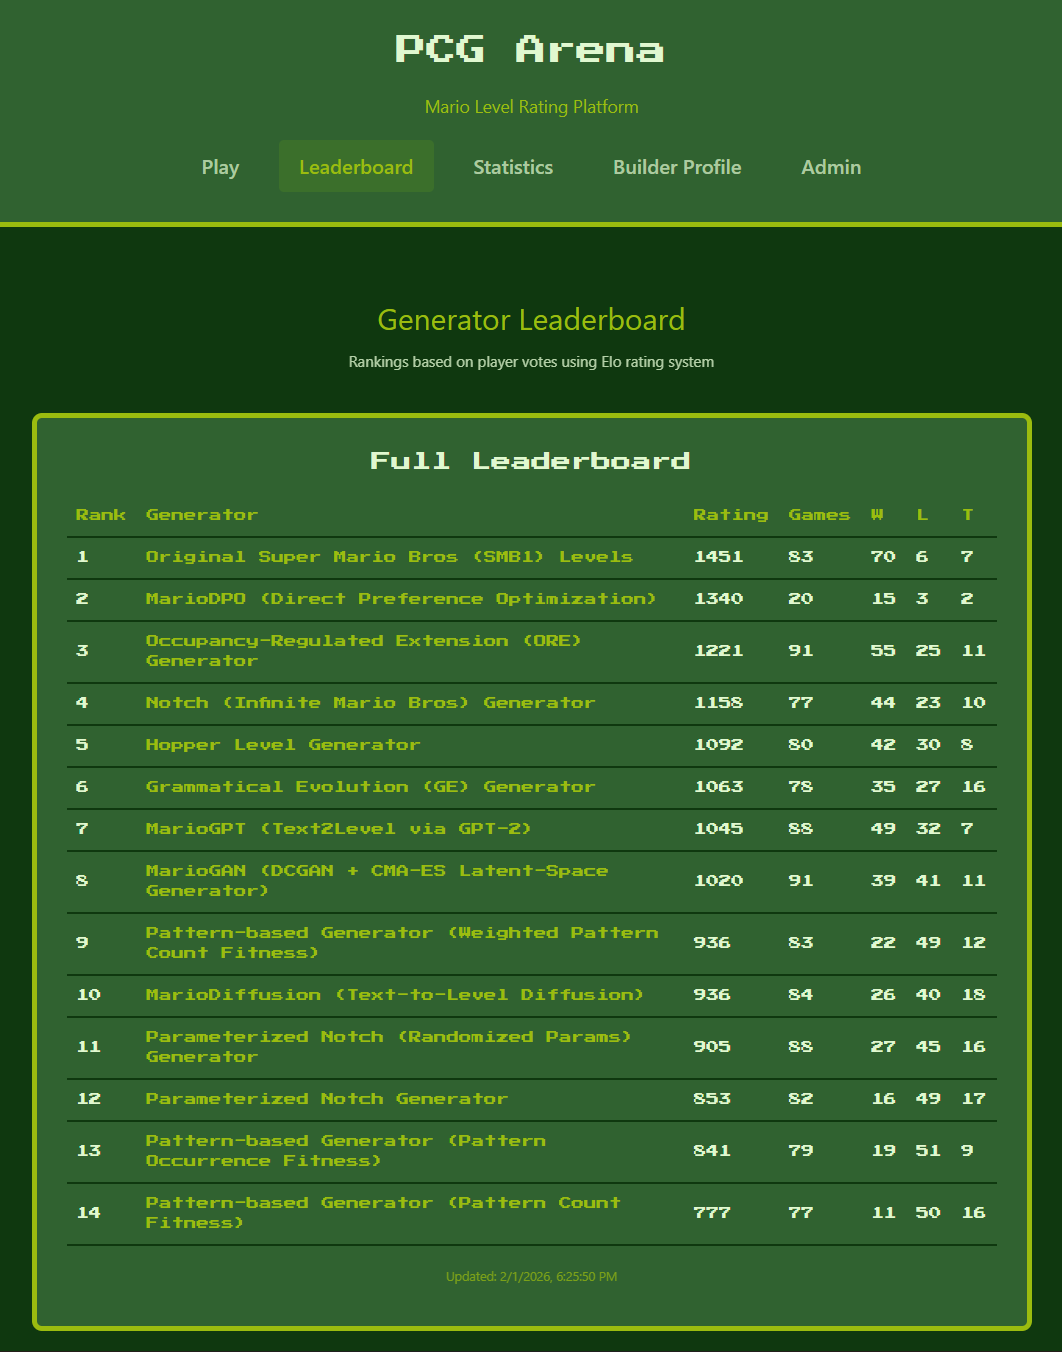
\includegraphics[width=0.85\textwidth]{MarioDPO_better_than_other_pcg.png}
\caption{MarioDPO compared with other procedural generators: it is the
strongest PCG method in the arena and the closest competitor to the original
human-authored levels.}
\label{fig:dpo-better-than-other-pcg}
\end{figure}

MarioDPO also improves substantially over MarioGPT (0.832 vs.\ 0.643), the checkpoint from which it was
initialised. Because both models share the same architecture and pretraining corpus, this gain comes directly from preference alignment on the arena data.

\section{Discussion}
\label{sec:dpo-discussion}

Three design choices account for MarioDPO's performance.

First, the base model starts from a strong structural prior. Reusing the
MarioGPT checkpoint and a column-major representation gives the generator a bias
toward valid, readable Mario geometry before preference optimisation begins. This avoids
a common failure mode of pure search or random generation, where the optimiser spends
most of its capacity rediscovering basic syntax.

Second, the judge function (Section~\ref{sec:dpo-judge}) supplies
broad negative coverage by flagging gap-fragmented and
uncompletable levels, so DPO sees many clear
negative examples while the human votes provide the positive preference signal.

Third, the preference dataset preserves the primacy of human judgement. Synthetic
pairs make the dataset large enough for DPO, but the 10$\times$ weight on human
votes ensures that the model is ultimately anchored to PCG Arena preferences.
This design is important because $J_{final}$ is only an approximation: it
reproduces the coarse quality tiering, but it cannot capture nostalgia,
aesthetic surprise, or all forms of level readability.

Together, these components close the loop that the platform was
built to enable. PCG Arena supplies human comparisons; the judge function turns
them into a scalable learning signal; and DPO converts that signal into a
generator whose levels reach human-authored quality. The exported levels are
packaged in the platform's seed format, ready for redeployment to gather the
fresh votes that would drive the next iteration of the same loop.


\chapter{Conclusions and Future Work}
\label{ch:conclusions}


\section{Summary of Contributions}
\label{sec:conc-contributions}

This thesis addressed the evaluation gap in procedural
content generation (the trade-off between scalable automated
metrics and valid human studies) through the design,
deployment, and analysis of PCG Arena, a web platform for blind
A/B testing of Super Mario Bros level generators.

\textbf{RQ1 (Measurement).} A persistent, blind, web-based arena can
produce a reliable human-preference ranking. The May 2026 export contains
1,000 pairwise votes from 77 anonymous player IDs over 14 generators, yielding
a stable leaderboard in which the human-authored \texttt{original} levels lead
(preference score 0.833) and pattern-based generators trail. Anonymous players largely agree on which generators perform well
(Section~\ref{sec:eda-user-heterogeneity}), so the aggregate ranking reflects a shared
preference signal.

\textbf{RQ2 (Metrics).} No. Automated structural metrics act as a
coarse filter, not a ranking: the four most-preferred generators have nearly
indistinguishable static profiles yet span almost 0.2 in preference score, and
no individual metric separates strong from weak generators
(Section~\ref{sec:eda-static-expressive-range}). By contrast, structural failure is measurable: frustrating, uncompletable levels appear consistently in
gameplay trajectories and player tags (Section~\ref{sec:eda-tag-semantics}). A heuristic judge
built on these failure indicators reproduces the coarse quality tiers in-sample
($r_s = 0.736$) and can label additional training pairs by filtering out
obvious failures.


\textbf{RQ3 (Generation).} The collected preferences suffice to train
a stronger generator: MarioDPO, fine-tuned with DPO on 473 human pairs and 2,606
judge-labelled synthetic pairs, achieves a preference score of 0.832,
nearly tied with the human-authored baseline (0.833) and ahead of
the next-best procedural generators, ORE (0.655) and MarioGPT (0.643).


In sum, the thesis contributes: (1)~PCG Arena, a persistent
open-access platform for blind pairwise evaluation of Mario level generators;
(2)~a user study of 1,000 blind votes across 14 generators; (3)~an exploratory
analysis pipeline linking votes to structure, behaviour, and tags; and
(4)~MarioDPO, a preference-aligned generator that approaches human-authored
quality.

\section{Limitations}
\label{sec:conc-limitations}

The findings of this thesis should be interpreted in light of several
methodological and technical limitations across the study protocol, the
platform design, and the preference-learning pipeline:

\begin{itemize}
    \item \textbf{Volunteer population and unknown player background.}
          Participation was voluntary and anonymous, tracked only via
          browser-based identifiers that can reset when cookies are cleared or
          devices change, and engagement was heavily concentrated in a small
          group of active contributors. Because no demographic or background
          survey was collected, we do not know participants' familiarity with
          platformer games or \emph{Super Mario Bros}, nor their general
          gameplay preferences, making it impossible to control for individual
          differences in skill or taste. Moreover, the platform does not model
          individual evaluator reliability (e.g., via play duration or decision
          latency).
    \item \textbf{Single-attempt protocol and immediate level transition.}
          Each level was evaluated after a single playthrough, and the second
          level in a battle started immediately after the first one ended,
          without giving the player a pause. While this design maximised the
          number of pairwise comparisons collected per unit of time, a player's
          own performance on that single attempt (such as an early mistake) may
          have influenced their rating, and the immediate transition between
          levels left no recovery pause between evaluations.
    \item \textbf{Unvalidated tag taxonomy and voting UI flow.}
          The selectable level tags were chosen based on what seemed
          appropriate for this study and do not constitute a validated
          instrument for evaluating game levels. Furthermore, the interface did
          not require players to select tags, and the tag selection option
          disappeared immediately after a player clicked their preferred level.
          While this flow encouraged rapid pairwise comparisons, it discouraged
          thorough qualitative evaluation and contributed to tag sparsity.
    \item \textbf{Presence of uncompletable levels.}
          Because level ingestion performed only format-level validation without
          automated reachability checks, the evaluation pool included levels
          that were impossible to complete. Encountering uncompletable levels
          may have frustrated human testers and negatively affected their
          motivation.
    \item \textbf{Recognisability of original levels.}
          Players familiar with the original Nintendo levels may have
          recognised them despite the blind setup, introducing a potential
          nostalgia or familiarity bias in favour of the human-authored
          baseline.
    \item \textbf{Dataset scale and judge bias in MarioDPO training.}
          The human preference dataset remains small by deep-learning standards,
          and the 2,606 synthetic pairs inherit the biases of $J_{final}$. In
          particular, judge features rely on short play sessions and A* agent
          simulations that do not fully reflect longer human exploration, and
          the style term privileges Nintendo-like structure, which may penalise
          innovative generators outside the original SMB1 distribution.
\end{itemize}

\section{Future Directions}
\label{sec:conc-future}

\begin{itemize}
    \item \textbf{Iterative retraining.} Train a MarioDPO-v2 on the May 2026
          export and study whether repeated collect--train--deploy cycles
          continue to improve preference scores.
    \item \textbf{Learned neural judge.} Replace the grid-searched
          $J_{final}$ with a neural preference model trained end-to-end on the
          growing vote corpus.
    \item \textbf{Beyond Mario.} Extend the arena protocol to other content
          domains to test the generality of blind pairwise evaluation of
          procedural generators.
    \item \textbf{Training-aware matchmaking.} Extend AGIS to select
          battles that are informative both for leaderboard ranking and as DPO training pairs.
\end{itemize}

\section[Closing Remarks]{Closing Remarks}
\label{sec:conc-closing}

The lesson of this thesis is that human taste does not
compress into a simple mathematical expression. Chapter~\ref{ch:eda} shows
this empirically: the generators players prefer most have static structural profiles that are nearly
indistinguishable from those of lower-ranked generators. Even the heuristic judge
of Section~\ref{sec:dpo-judge}, calibrated specifically on this dataset,
primarily identifies clear structural failures.

This offers an explanation for a long-standing pattern in the field.
For much of the last two decades, procedural level generation has been driven
by explicit objectives: fitness functions in search-based PCG, reward functions
in PCGRL, hand-tuned metrics such as leniency and linearity. Each encodes a
designer's hypothesis about what makes content good, and each is falsifiable in
the same way---a generator can maximise the objective and still produce levels
players do not enjoy, which is precisely what \citet{marino2015empirical}
observed and what the present data reproduces at larger scale. The difficulty
was never a shortage of optimisation power; it was that the objective being
optimised was a guess about human preference, not a measurement of it.

MarioDPO takes the opposite route. It never represents ``fun''
explicitly. It collects pairwise judgements from players and lets Direct
Preference Optimisation shape the generator directly from those comparisons,
using the judge only to supply broad negative coverage. The result is a
generator that reaches a preference score of 0.832, statistically
indistinguishable from hand-authored Nintendo levels at 0.833, and ahead of the
MarioGPT checkpoint it was initialised from---improvement obtained by
alignment alone, without changing the architecture or the training corpus.

Nothing in this pipeline is specific to Super Mario Bros. It requires
a domain where content can be presented in pairs, a population willing to state
which of two artefacts they prefer, and a generative model that can be
fine-tuned on those preferences---conditions that hold for dungeons, tracks,
quests, textures, and most other PCG domains. The contribution of this thesis
is therefore not only a stronger Mario generator, but evidence for a general
recipe: stop trying to write down what players enjoy, and start measuring it.

\section*{Statement on the Use of AI Tools}

The thesis was written by the author, who is not a native speaker of English. Large
Language Models, including models from OpenAI, Google, and Anthropic, were used to 
improve English style, clarity, and phrasing after the text had
been drafted by the author. These tools were also used as support in preparing
plots and figures. AI-assisted tools were also used during development as part of the
author's programming workflow. The author remains responsible for the research
design, implementation choices, experiments, analysis, and final content of the thesis.




\bibliographystyle{plainnat}
\bibliography{bibliography}

\end{document}
